\documentclass[twoside,11pt,fleqn]{memoir}%%% seminario planetari PPS
%openany

%% rimuove workout errata dalla versione da consegnare
\def\versione{bozza}%%VERSIONE
\def\bozza{bozza}
\def\consegna{consegna}
%%%PENALITIES
%\widowpenalty=10000
%\clubpenalty=10000
%% colors
\usepackage[usenames,dvipsnames]{xcolor}
\definecolor{antiquefuchsia}{rgb}{0.57, 0.36, 0.51}
\definecolor{violetw}{rgb}{0.93, 0.51, 0.93}
\definecolor{Veronica}{rgb}{0.63, 0.36, 0.94}
\definecolor{atomictangerine}{rgb}{1.0, 0.6, 0.4}
\definecolor{darkgray}{rgb}{0.66, 0.66, 0.66}
\definecolor{brightcerulean}{rgb}{0.11, 0.67, 0.84}
\definecolor{cadmiumorange}{rgb}{0.93, 0.53, 0.18}
\definecolor{ochre}{rgb}{0.8, 0.47, 0.13}
\definecolor{midnightblue}{rgb}{0.1, 0.1, 0.44}
\definecolor{grey}{rgb}{0.7, 0.75, 0.71}
\definecolor{bf}{RGB}{88, 86, 88}
\definecolor{bb}{RGB}{177, 177, 177}
%%indice analitico: necessari per printindex
\usepackage{makeidx}
\makeindex
%%%%%%%%%%%%%%%%%%%%%%%%%%%%%%%%%%% importa pacchetti
\usepackage{usepkg}
%%%%%%%%%%%%%%%%%%%%%%%%%%%%%%%%%%%%%
\addtocontents{toc}{\cftpagenumbersoff{part}} %% part senza numero pagina in toc
%%%%%%%%%%%%%%%%%% titletoc, titlesec setting.
%%%%%%%%%%%%%%%%%%      pagestyle
\usepackage{titleT}
\pagestyle{plain}
%%%%%%%%%%%%%%%%%% length
\usepackage{length}
%%%%%%%%%%%% Hyperref package
\usepackage{hyperref}
\hypersetup{
    colorlinks,
    citecolor=black,
    filecolor=black,
    linkcolor=black,
    urlcolor=black
}
%%%%%%%%%%%%%%%%%%%%%%%% Things need to be loaded after hyperref
%\usepackage{cleveref}
%%%%%%%%%%%%%%%%%Geometry package
\usepackage[a4paper,lmargin=80px,rmargin=40px,tmargin=40px,bmargin=20px,nofoot,footskip=20px]{geometry}
%http://tex.stackexchange.com/questions/211248/problem-with-cropmarks-on-geometry-package
%http://www.ctex.org/documents/packages/layout/geometry.pdf
%%%%%%%%%%%%%%%%%%%%%%%%%%%%%%%%%%% Funzioni generali
\usepackage{functions}
%http://tex.stackexchange.com/questions/246/when-should-i-use-input-vs-include
\usepackage{sources}
%%%%%%%%%%%%%%%%%%%%%%%%%%%%%%%%%%% Funzioni per questo file main
\usepackage{mathOp}
\usepackage{LocalF}
\usepackage{ads}
%%%%%%%%%%%%%%%%%%%%%%%%%%%%%%%%%
\raggedbottom %http://tex.stackexchange.com/questions/102084/annoying-paragraph-spacing-issue-with-memoir
%% CAption subcaption figure %%% captionsetup
%\captionsetup[subfigure]{labelformat}
    \makeatletter
    \renewcommand\@memmain@floats{%
      \counterwithout{figure}{section}
      \counterwithout{table}{section}
  \counterwithout{figure}{chapter}
    \counterwithout{figure}{subfigure}
      \counterwithout{table}{chapter}
      \counterwithin{figure}{part}
      \counterwithin{table}{part}
	\renewcommand{\thesubfigure}{\arabic{part}-\arabic{figure}.\alph{subfigure}}
	\renewcommand{\thefigure}{\arabic{part}-\arabic{figure}}
	\renewcommand{\thetable}{\arabic{part}-\arabic{table}}
      }
    \makeatother
%%%%
%%% SOlve page pre chapter at begginning page without number%@ps
\chapterstyle{plain}
%%%
%\makeatletter
%\newcommand{\titolo}{\@title}
%\makeatother
\author{ }
\title{Simulazione popolazioni planetarie}
\date{\today}
%%%
%\outputonly{1}% output in pdf only page number
\begin{document}
\maketitle
\pagenumbering{roman}
\tableofcontents*
\mainmatter
\pagenumbering{arabic}
\aliaspagestyle{chapter}{plain}
\cleartorecto
%%Intro
Il crescente numero di esopianeti osservati ha stimolato lo studio dei processi di formazione dei sistemi planetari tramite modelli di formazione globale: 
I modelli di formazione planetaria fino alla scoperta del primo esopianeta (Queloz 1995) erano vincolati a riprodurre le caratteristiche peculiari del sistema

{\let\clearpage\relax\let\cleardoublepage\relax
\part{Vincoli ai modelli di formazione planetaria}
}
Descrivo le tecniche osservative, le osservabili e effetti di selezione, quindi le propriet\'a degli esopianeti nei diagrammi $(a-M)$, $(a-R)$, $(M-R)$: quali osservabili determinano le diverse tecniche osservative, struttura pianeta (sistema solare, esopianeti).
\begin{workout}[vincoli e condizioni iniziali: less modell dependent that I can]
\begin{itemize}
\item SISTEMA SOLARE
\item[-] Datazione: tempi scala formazione
\item[-] struttura orbitale e composizione sistema solare: MMSN
\item[-] composizione pianeti
\item[-] modelli sistema solare: walsh 11 (grand tack) (with comparison with exoplanets??)
\item ESOPIANETI
\item[-] Survey osservativi e completezza
\item[-] diversity: distribuzione di massa-distribuzione bimodale per piccole/grandi masse con minimo a $30\mearth$, crescita esponenziale a basse masse, secondo picco a masse gioviane
\item[-] distribuzione  raggio/densit\'a: eos, evaporazione, composizione
\item[-] Propriet\'a statistiche esopianeti: ??
\item Dischi protopalnetarii
\item[-] Osservazioni: distribuzione di massa, tempo di vita e condizioni iniziali e metallicit\'a stellare.
\item[-] Modello di disco di accrescimento
\end{itemize}
\end{workout}
% trim={5cm 0 0 0},clip
%vincoli e condizion iniziali per pps??
{\let\clearpage\relax\let\cleardoublepage\relax
\chapter{Sistema solare}
}

\begin{workout}[Vincoli ai modelli di formazione: sistema solare]
Struttura e composizione pianeti: orbite su un piano quindi disco accrescimento, chiarire et\'a del sistema solare/Sole e tempi scala CA/GI; tempi scala formazione e migrazione giove saturno: late haevy bombardament. Massa minima disco protoplanetario. Modello pianeti gassosi per determinare profilo densit\'a e quindi composizione.
\end{workout}

Il sistema solare \'e il punto di partenza delle teorie di formazione planetaria; infatti si hanno informazioni accurate sui pianeti e loro orbite, sulla popolazione di corpi minori e, tramite datazione radiochimica, si hanno riferimenti temporali sui tempi di formazione della componente solida.

L'et\'a del Sole \'e definita come tempo in sequenza principale: tecniche eliosismologiche determinano un'et\'a di \SI{4.57+-0.11}{\giga\year} (\cite{bonanno2002age}) mentre l'analisi chimica dei meteoriti \SI{4.57+-0.07}{\giga\year} (\cite{bahcall1995solar}).
Il core terrestre si \'e formato completamente circa \SIrange{10}{29}{\mega\year} dopo i meteoriti (\cite{yin2002short}).

\begin{workout}[Massa disco proto solare: weidenschilling/Hayashi]
W: $M\approx0.01-0.1\msun$, H: $M\approx0.013\msun$
\end{workout}

\begin{workout}[accrescimento di gas su nucleo solido prevede arricchimento di metalli ]

\end{workout}

\begin{workout}[caratteristiche orbitali sistema solare]
	\begin{table}[!ht]
		\pgfplotstabletypeset[%skip rows between index={4}{8},
		every head row/.style={
			before row={\midrule},
			%every last row/.style={after row=\bottomrule},
			after row={\midrule}
		},
		every 2 row/.style={after row=\midrule},
		every last row/.style={after row=\bottomrule},
		every first column/.style={column type/.add={|}{}},
		every last column/.style={column type/.add={}{|}},
		%columns/0/.style = {column type/.add={|}{}},
		%columns/5/.style = {column type/.add={|}{}},
		%columns/0/.style={string type},
		create on use/majoraxis/.style={
			create col/expr={\thisrow{a}/1.5}},
		display columns/1/.style={fixed,column name={$a(AU)$},clear infinite},
		display columns/2/.style={column name={e},clear infinite},
		display columns/3/.style={column name={i},clear infinite},
		display columns/4/.style={column name={$\tau_{sid}(\si{\hour})$},clear infinite},
		display columns/5/.style={column name={obliquity},clear infinite},
		display columns/planets/.style={column name={pianeta},string type},
		create on use/planet/.style={create col/set list={Mercury, Venus, Earth, Mars,Jupiter,Saturn,Uranus,Neptune}},
		columns/planet/.style={string type},
		columns={planet, majoraxis, e, i, Ps, obl},
		/pgf/number format/precision=3
		]{solarsystemmain-orbit.txt} %%%
		\captionof{table}{Caratteristiche pianeti del Sistema solare.}\label{tab:terrestrial planets}
	\end{table}
\end{workout}

%La formazione per accrescimento di gas su nucleo solido prevede arricchimento di metalli rispetto alla composizione di partenza.
La composizione dei pianeti giganti \'e determinata grazie a modelli di struttura planetaria. Vincoli alla distribuzione di massa interna sono imposti dalla misura dei momenti di multipolo del potenziale gravitazionale: risolvendo un modello di pianeta che rientri nei vincoli osservativi si determinano la massa del core e la metallicit\'a dell'inviluppo gassoso dei 4 pianeti gassosi (vedi  tabella \ref{tab:JSUNcomp}).

\begin{table}[!htb]
    \begin{minipage}{.5\linewidth}
      \centering
        \begin{tabular}{|ccc|}
\hline
&\parbox{1.5cm}{Jupiter $317.8\mearth{}$}&\parbox{1.5cm}{Saturn $95.1\mearth{}$}\\
  $M_c$&$0-11\mearth{}$&$9-22\mearth{}$\\
\hline
$M_Z$&$1-39\mearth{}$&$1-8\mearth{}$\\
\hline
$M_Z^{tot}$&$8-39\mearth{}$&$13-28\mearth{}$\\
\hline
$Z/Z_{\odot}$&$1-6$&$6-14$\\
\hline
 \end{tabular}
    \end{minipage}%
    \begin{minipage}{.5\linewidth}
      \centering
        \begin{tabular}{|ccc|}
\hline
&\parbox{1.5cm}{Uranus $14.5\mearth{}$}&\parbox{1.5cm}{Neptune $17.1\mearth{}$}\\
\hline
$M_{rock}$&$3.7\mearth{}$&$4.2\mearth{}$\\
\hline
$M_{ice}$&$9.3\mearth{}$&$10.7\mearth{}$\\
\hline
$M_{H/He}$&$1.5\mearth{}$&$2.2\mearth{}$\\
\hline
        \end{tabular}
    \end{minipage} 
    \caption{Composizione Giove, Saturno: $M_c$ \'e la massa del core, $M_Z$ la massa di metalli nell'inviluppo gassoso, $M_Z^{tot}$ la massa totale di metalli; composizione di Urano e Nettuno. Da \cite{baraffe2009physical}.}\label{tab:JSUNcomp}
\end{table}

\begin{wrapfigure}[6]{r}{0.5\textwidth}
	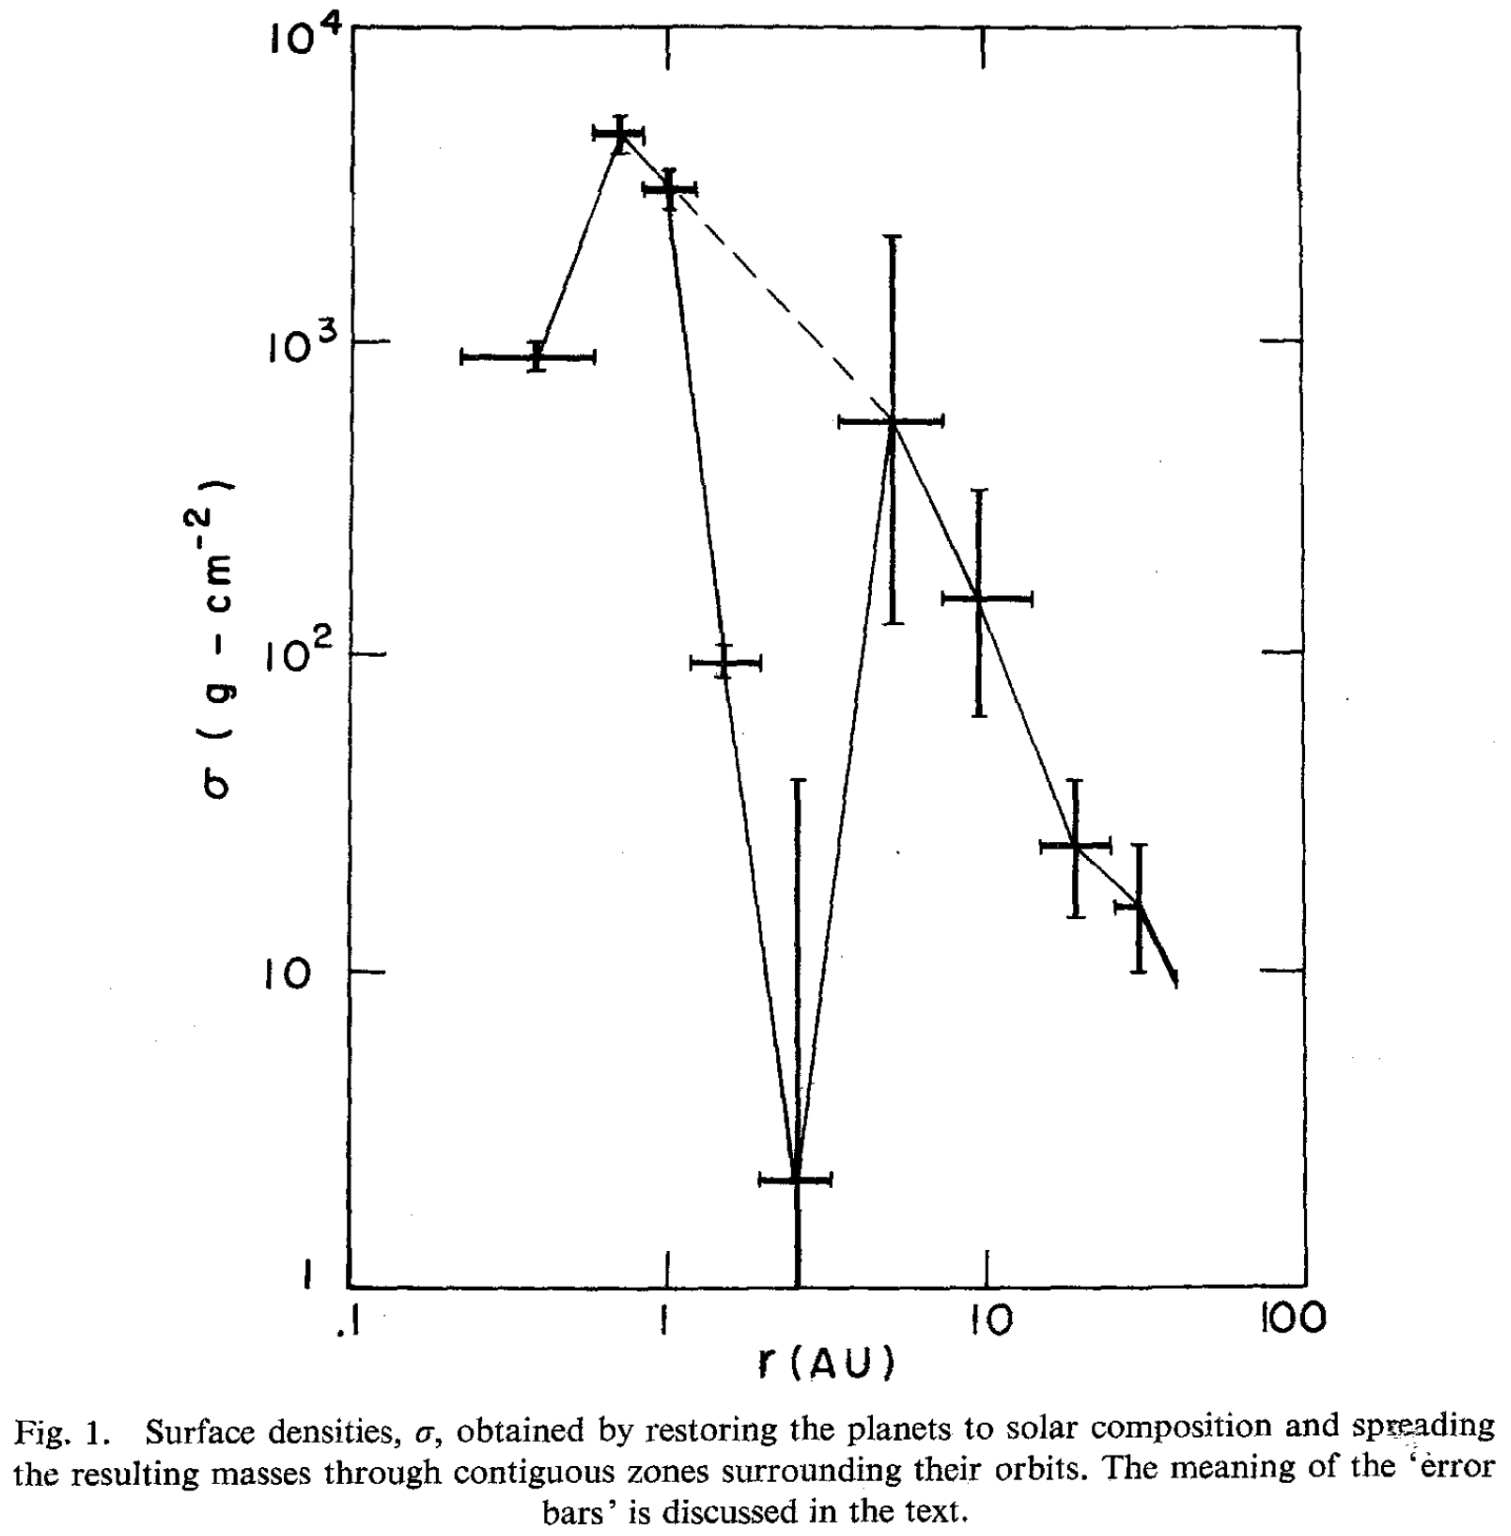
\includegraphics[trim={0cm 5cm 0 0cm},clip, width=0.5\textwidth]{Snebuladensity}\caption{Andamento minimum mass solar nebula (MMSN). Da \cite{weidenschilling1977distribution}.}\label{fig:Snebuladensity}
\end{wrapfigure}

Un limite inferiore alla massa del disco protoplanetario si ottiene  considerando la massa presente nei pianeti e nella fascia asteroidale arricchita di H/He per avere composizione solare e distribuendo questa massa in un anello di spessore proporzionale al raggio di Hill e centrato sulle orbite (\cite{weidenschilling1977distribution}): si ha l'andamento della densit\'a superficiale, proporzionale a $r\expy{-3/2}$, mostrato in figura (\ref{fig:Snebuladensity}); (\cite{hayashi1981structure}) ha determinato l'andamento della densit\'a di gas, ghiaccio e rocce:
%$\Sigma\propto r\expy{-3/2}$.
\begin{align}
&\Sigma_{rock}=7.1(\frac{a}{\si{\astronomicalunit}})\expy{-3/2}\si{\gram\per\square\cm}:\ \frac{a}{\si{\astronomicalunit}}=0.35-2.7\\
&\Sigma_{rock+ice}=30(\frac{a}{\si{\astronomicalunit}})\expy{-3/2}\si{\gram\per\square\cm}:\ \frac{a}{\si{\astronomicalunit}}=2.7-36\\
&\Sigma_{gas}=\num{e3}(\frac{a}{\si{\astronomicalunit}})\expy{-3/2}\si{\gram\per\square\cm}:\ \frac{a}{\si{\astronomicalunit}}=0.35-36
\end{align}

Per riprodurre alcune importanti caratteristiche del sistema solare \'e stato necessario considerare fenomeni di migrazione dovuti a scambio di momento angolare con gas e planetesimi:
\begin{itemize}
	\item  il modello di Nizza del sistema solare (\cite{tsiganis2005origin}) riproduce l'eccentricit\'a e l'inclinazione dei pianeti giganti considerando l'attraversamento della risonanza $2:1$ tra Giove e Saturno dovuta a migrazione in disco di planetesimi (\cite{hahn1999orbital})
	\item considerando la migrazione prodotta da interazione gravitazionale tra pianeti giganti e gas del disco protoplanetario (\cite{lin1986tidal}) lo scenario del grande Tack (vedi \cite{walsh2011low}) considera la formazione di Giove e sua migrazione verso l'interno finch\'e a \SI{1.5}{\astronomicalunit} la cattura di Saturno in risonanze $2:3$ causa inversione della migrazione; la distanza di inversione della migrazione di Giove \'e determinata da simulazioni numeriche che mostrano che una distribuzione di planetesimi troncata a 1 AU (\cite{hansen2009formation}) riproduce la struttura orbitale dei pianeti terrestri. In questo scenario si riproduce la distribuzione della composizione degli oggetti nella fascia degli asteroidi.
\end{itemize}

%riproduce caratteristiche orbitali dei pianeti giganti considerando la loro migrazione in una distribuzione di planentesimi di $30-50\mearth{}$ ; 
%la presenza di numerosa popolazione di planetesimi \'e corroborata dalla craterizzazionedei pianeti terrestri e corpi minori come dall'esistenza di numerosi oggetti di piccole dimensioni superstiti.

\begin{workout}[Cosa dire dei modelli planetarii: core giganti gassosi: modelli planetari e raffronto isolation mass in MMSN]
parte relativa ai momenti multipolo gravitazionale. 
In hydrostatic equilibrium the external gravitational potential is
\begin{align}
&V(r,\theta)=\frac{GM_p}{r}[1-\sum_1^{\infty}(\frac{R_+}{r})^{2n}J_{2n}P_{2n}(\theta)]\\
&J_{2n}=-\frac{1}{M_pR_+^{2n}}\int\rho(r) r\expy{2n}P_{2n}(\theta)\,d^3r
\end{align}
zharkov trubitsyn 74
Noble gas enrichment: ''FORMATION OF GIANT PLANETS ? AN ATTEMPT IN MATCHING OBSERVATIONAL CONSTRAINTS''
Degree of super-adiabaticity: Struttura interna (assimption for pre-runaway accretion)
See: characterization of exoplanets from their formation (pg4)
Degree of super-adiabaticity: baraffe 02, Rafikof 07
\end{workout}

\begin{workout}[Planetesimal and late heavy bombardament]
??
\end{workout}

\begin{workout}[Ages]
Stellar age: isochrone fitting: Jorgensen Lindegren 05.
Earth age pg 297; allegre 95.
et\'a corpi sistema solare (age and chronology): age of the sun  $4.57Gyr$ (Bahcall95); CAI: $4567Myr$ +3Myr chondrule
\end{workout}

\begin{workout}[few well separeted homogeneous region: Struttura interna (assimption for pre-runaway accretion)]
See: characterization of exoplanets from their formation (pg4)
Baraffe 07: composition gradients, core dissolution: Wilson, Militzer 12, planetesimal deconstruction: mordasini 05, multiconvective layers: Leconte chabrier 12.
\end{workout}

\begin{workout}[Solar system orbital properties]
Full packing/spacing

Planetesima migration: pluto eccentricity, large population of Kuiper belt object

Orbit of terrestrial planets]
Constrain for core accretion model ofgiant planets: dynamical shakeup Nagasawa 05 Thommes08c

Planet obliquity:
Schlichting sari 07: The effect of Semi-Collisional Accretion on Planetary Spins
Inconsistent with isotropic distro (Tremaine 1991). Randomly directed component of spin angular momentum (Kokubo Ida 07) cause large then observed i,e (Harris Ward 82).
Planetesimal/protoplanet collision would imply stachastic rather than smooth accretion.
Excittion of giant planet spin obliquity if spin axis precession freq pass through resonance with orbital prec freq during migration.
Uranus: tilt due to collision or migration: Bergstralh 91 or Bou\'e Laskar 10.
Non of obliquity of terrestrial planet are belived primordial (secular orbit perturbation)+tidal dissipation.
Effects of inhomogenous infall on obliquity (tremaine 91, bate 10)
\end{workout}

{\let\clearpage\relax\let\cleardoublepage\relax
	\chapter{Dischi protoplanetari: struttura e condizioni iniziali per simulazione formazione pianeti}
}

%\section{Modello disco di accrescimento }
Per riprodurre le propriet\'a statistiche della popolazione planetaria osservata \'e fondamentale determinare la distribuzione delle caratteristiche dei dischi di accrescimento che, combinate usando metodi di Montecarlo, vanno a costituire le condizioni iniziali dei modelli di formazione. Osservando cluster di stelle in in formazione \'e possibile ricavare la distribuzione di massa e raggio carateristico dei dischi protoplanetari e del tempo di vita.

%Tramite metodi di montecarlo si determinano numerose combinazioni delle condizioni iniziali del disco e dei parametri scelti per descrivere la sua struttura.
%Le variabili di montecarlo hanno distribuzione determinata dalle osservazioni.

Nei modelli di disco di accrescimento $1+1D$ si parametrizza il trasporto di momento angolare ponendo:
\begin{equation}
\nu=\alpha c_s H
\end{equation}
dove $\alpha$ \'e parametro da fissare, $c_s$ la velocit\'a del suono e H lo spessore del disco; si ipotizza che la turbolenza sia responsabile per la viscosit\'a aumentata quindi che la velocit\'a relativa dei moti turbolenti sia circa la velocit\'a del suono $c_s$ e la dimensione caratteristica lo spessore del disco $H$. L'evoluzione della densit\'a superficiale del disco \'e quindi determinata dall'equazione:
\begin{equation}
\PDy{t}{\Sigma}=3\frac{1}{r}\PDof{r}[r\expy{1/2}\PDof{r}(\nu\Sigma r\expy{1/2})]\label{eq:sigmaevol}
\end{equation}

La struttura verticale \'e determinata dalla componente lungo z dell'attrazione del corpo centrale
%profilo termico determinato da equilibrio termico
\begin{equation}
\TDy{z}{P}=-\rho g_z=-\frac{GM_*}{r^2+z^2}\frac{z}{r}\rho=-\Omega^2\rho z\label{eq:hydroz}
\end{equation}
mentre la struttura radiale del disco di gas \'e determinata dall'equilibrio idrostatico
\begin{equation}
\frac{v_g^2}{r}=\frac{GM_*}{r^2}+\frac{1}{\rho}\TDy{r}{P}
\end{equation}
dove ho introdotto $v_g$ velocit\'a a cui il gas orbita attorno alla stella centrale.

\begin{wrapfigure}[10]{l}{0.4\textwidth}
	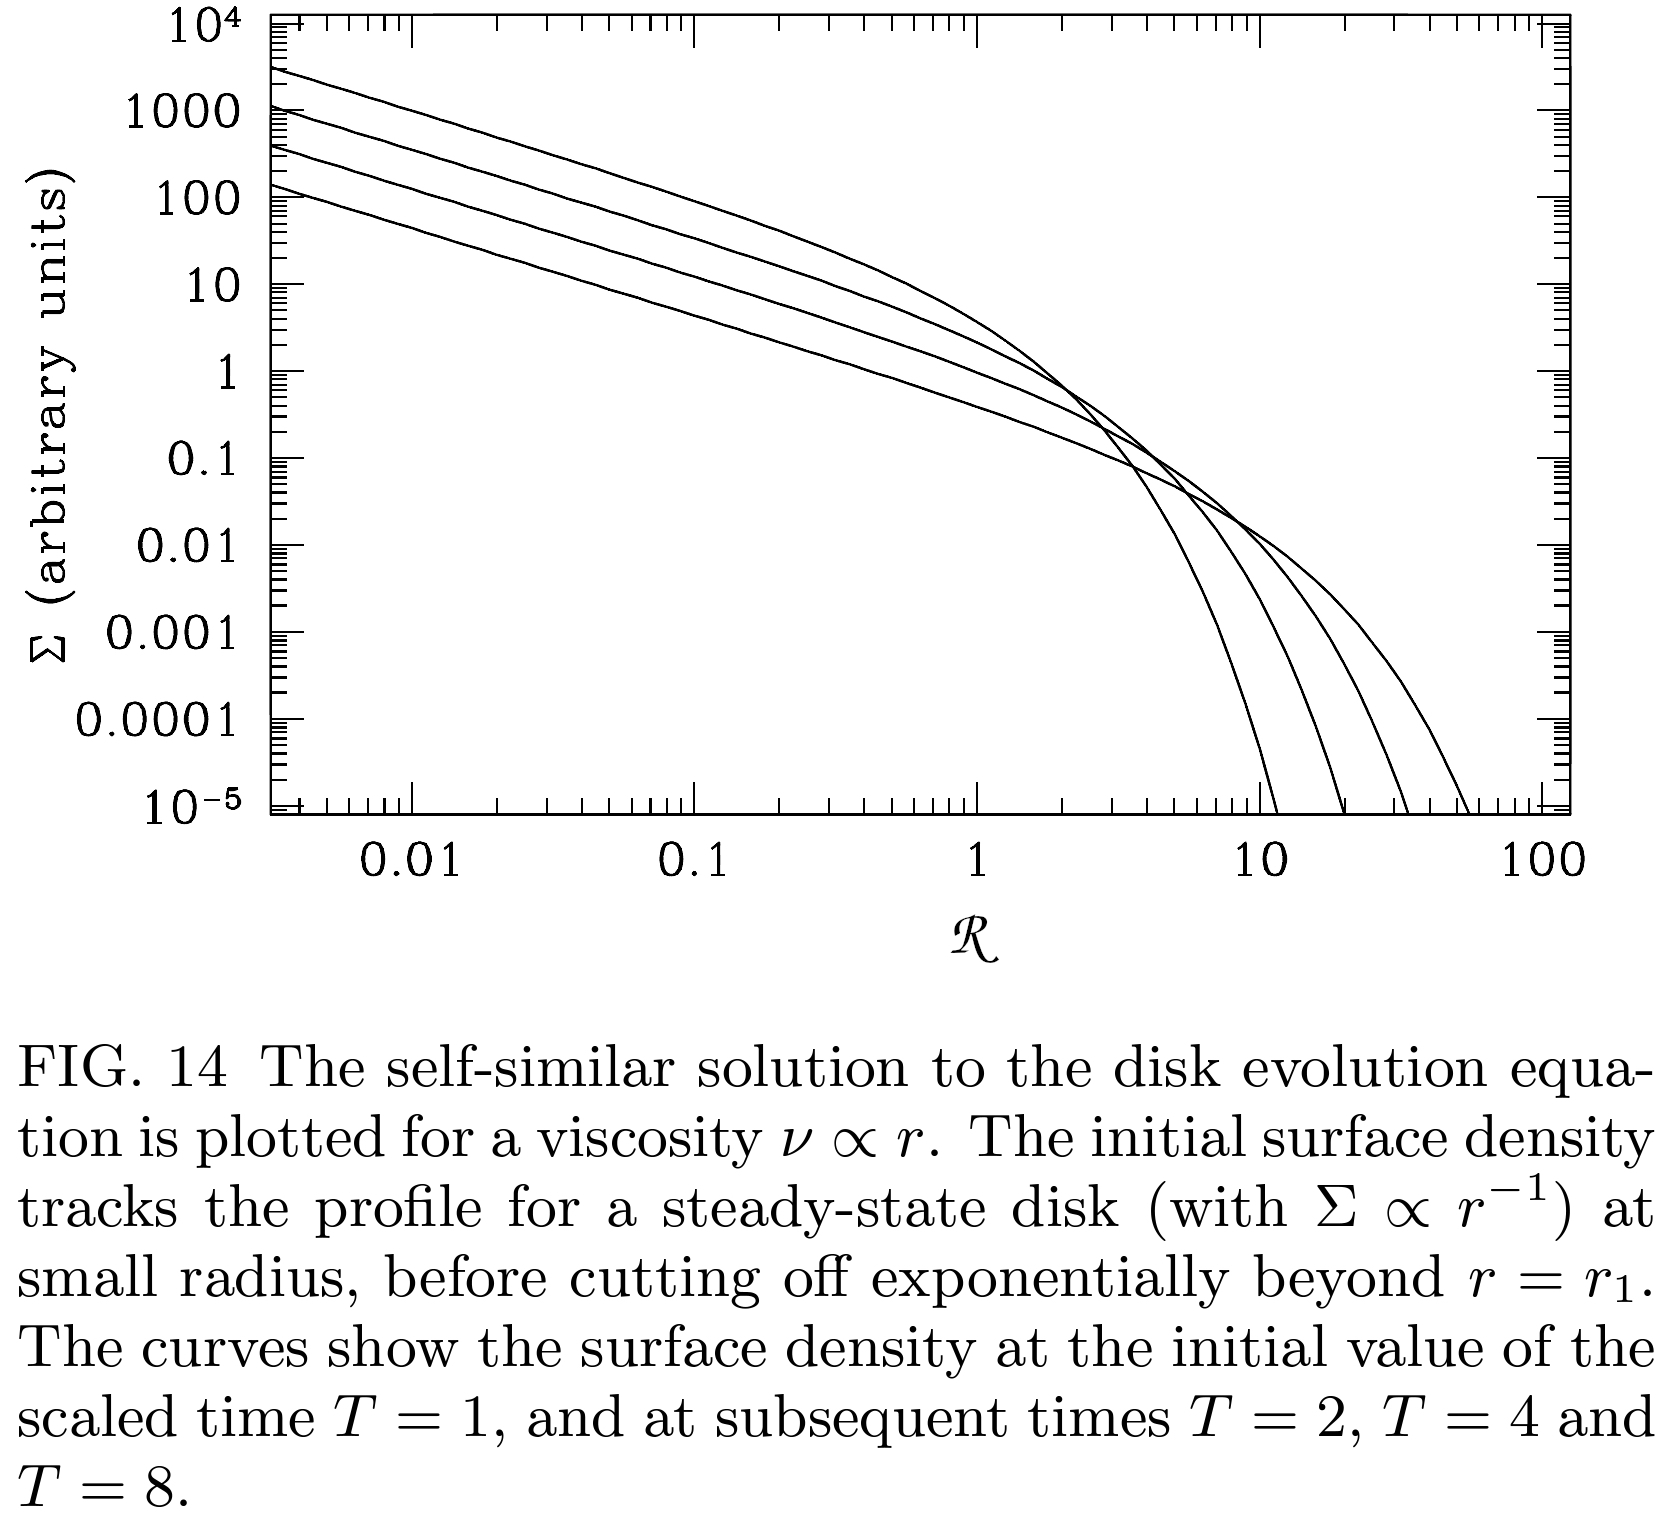
\includegraphics[trim={0cm 4cm 0 0},clip, keepaspectratio,width=0.4\textwidth]{selfsimilaralphadisk-mod}
	\caption{I grafici rappresentano densit\'a superficiale \eqref{eq:selsimdiskevol} per $\nu\propto r\expy{\gamma}$ con $\gamma=1$: $T=2,4,8$. Da \cite{armitage2007lecture}.}\label{fig:selfsimilaralphadisk}
\end{wrapfigure}

La soluzione auto-similare di( \ref{eq:sigmaevol}) con raggio caratteristico $R_c$, assumendo $\nu\propto r\expy{\gamma}$, \'e
\begin{equation}
\Sigma(\mathcal{R},\mathcal{T})\propto\mathcal{R}\expy{-\gamma}\mathcal{T}\expy{-\frac{5/2-\gamma}{2-\gamma}}\exp{-\frac{\mathcal{R}\expy{2-\gamma}}{\mathcal{T}}}\label{eq:selsimdiskevol}
\end{equation}
con
\begin{align}
&\mathcal{R}=\frac{r}{R_c}
&\mathcal{T}=\frac{t}{t_c}\ t_c=\frac{1}{3(2-\gamma)^2}\frac{R_c^2}{\nu(R_c)}
\end{align}

Il profilo termico \'e determinato assumendo che l'energia prodotta da viscosit\'a sia trasportata radiativamente alla superficie:
\begin{equation}
\PDy{z}{F}=\frac{9}{4}\rho\nu\Omega^2\label{eq:energyeq}
\end{equation}
infine per un disco otticamente spesso si ha
\begin{equation}
F=-\frac{16\pi\sigma T^3}{3\kappa\rho}\PDy{z}{T}\label{eq:radtransport}
\end{equation}
Le condizioni al contorno per le equazioni (\ref{eq:hydroz}), (\ref{eq:radtransport}), (\ref{eq:energyeq}) (vedi \cite{benz2014planet}):
\begin{align}
&P_s=\frac{\Omega^2H\tau_{ab}}{\kappa_s}\\
&F_s=\frac{3}{8\pi}\dot{M}_*\Omega^2\\
&2\sigma(T_s^4-T_b^4)-\frac{\alpha kT_s\Omega}{8\mu m_H\kappa_s}-\frac{3}{8\pi}\dot{M}\Omega^2=0\\
&F(z=0)=0
\end{align}
dove pedice s significa che la quantit\'a \'e valutata alla superficie $z=H$, $\tau_{ab}$ \'e la profondit\'a ottica dalla superficie del disco a infinito, $T_b$ \'e la temperatura di background; il rate di accrescimento \'e
\begin{equation}
\dot{M}=3\pi\nu_{eff}\Sigma,	\quad\nu_{eff}=\frac{\int_{-H}^H\nu\rho\,dz}{\Sigma}
\end{equation}
Per tenere conto della radiazione della stella centrale si pone:
\begin{equation}
T_s^4=T_{s,noirr}^4+T_{s,irr}^4
\end{equation}

\begin{figure}[!ht]
	\begin{subfigure}[b]{0.39\textwidth}
		\centering
		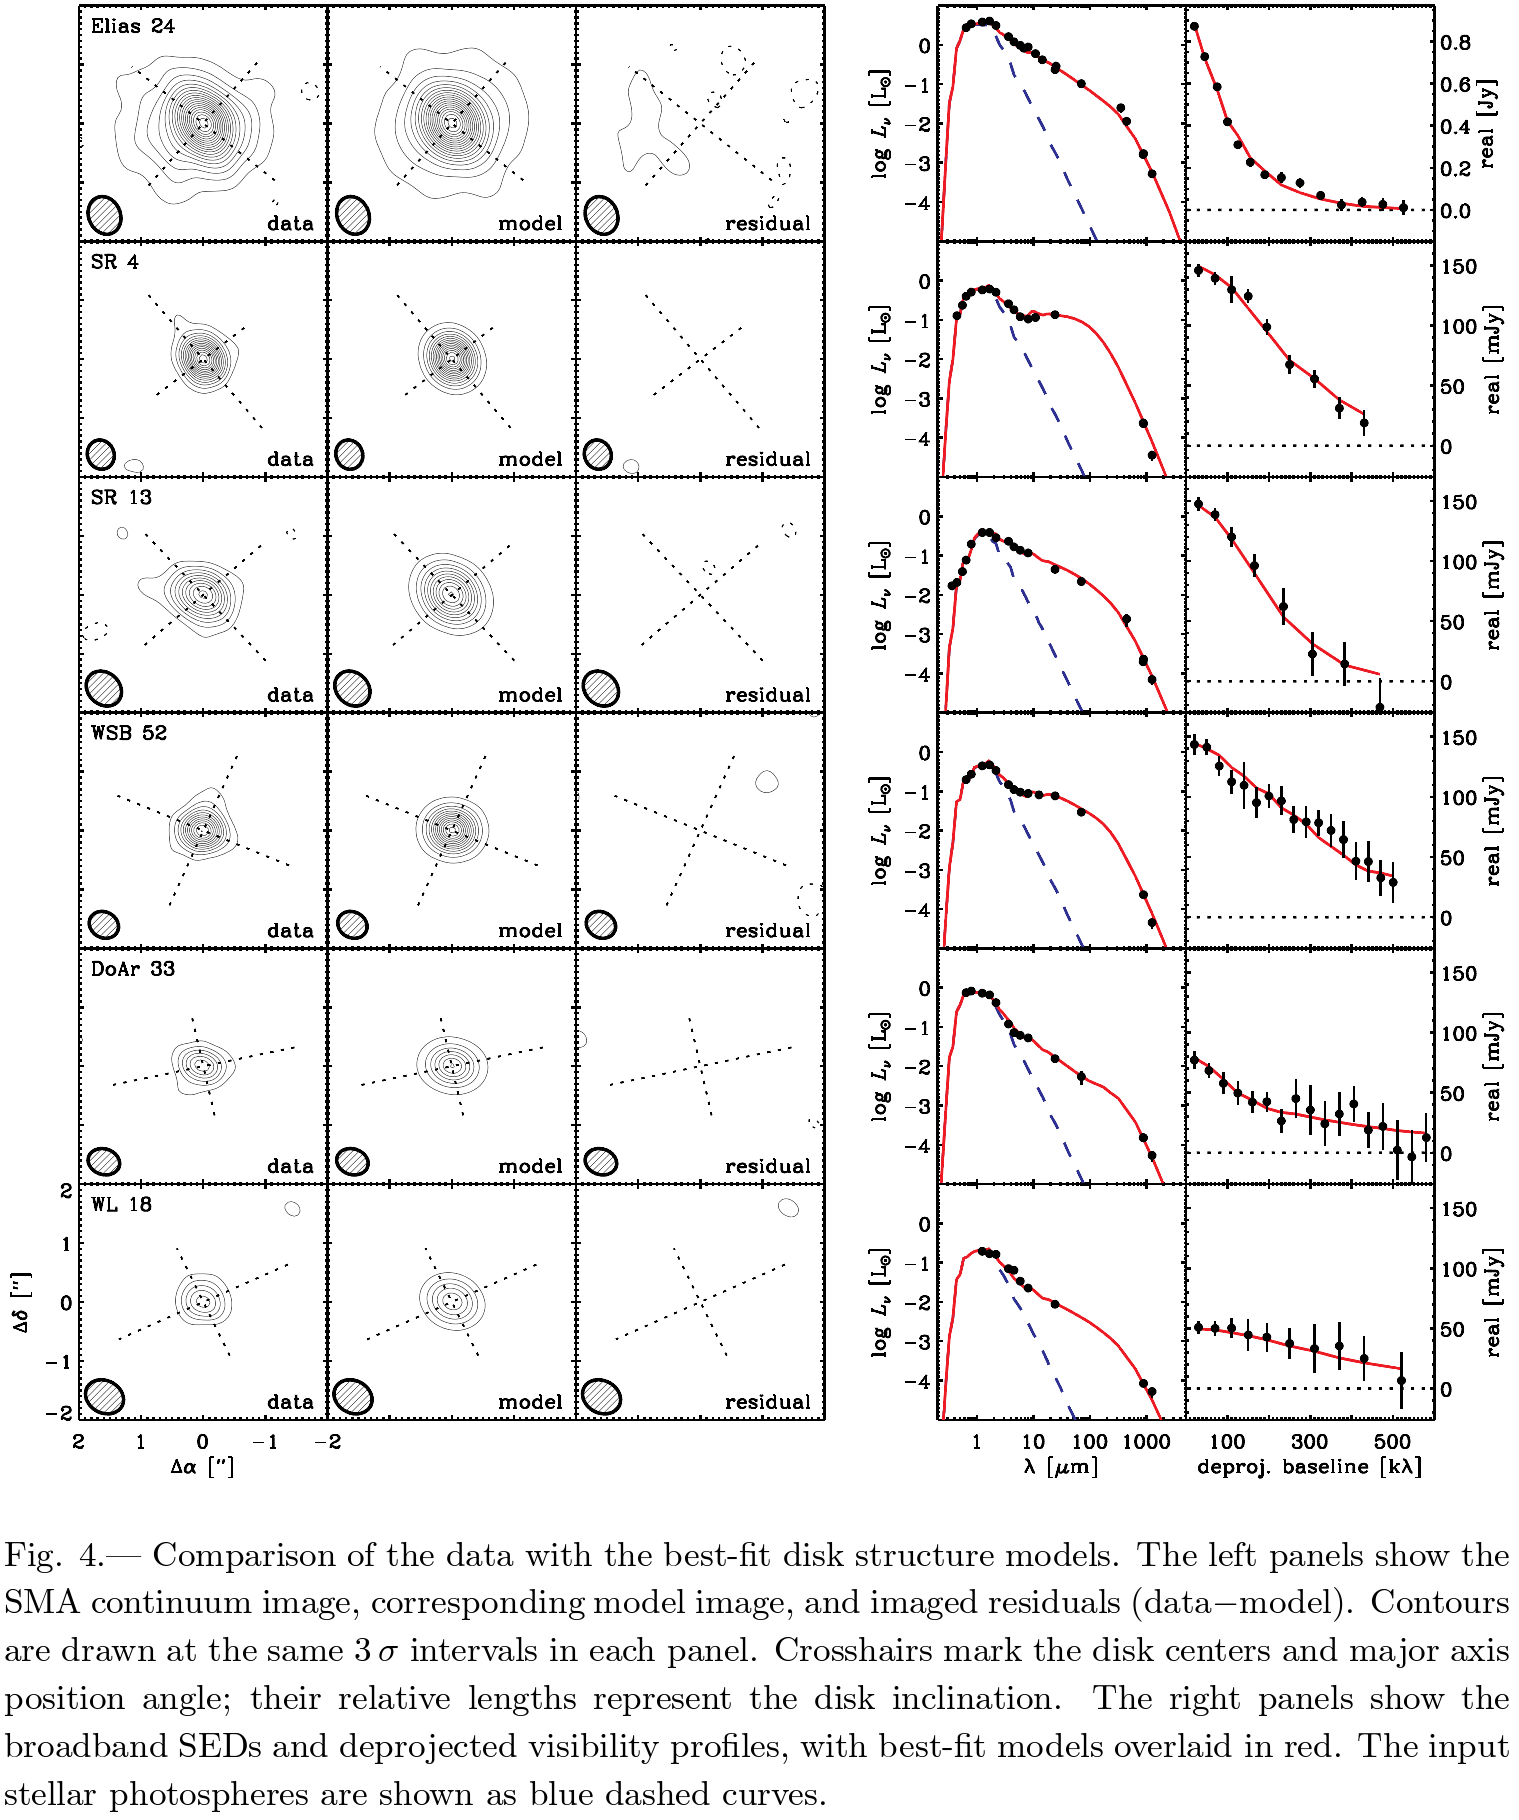
\includegraphics[trim={0cm 10cm 0 0},clip, keepaspectratio,width=0.98\textwidth]{SED-contours}
		\caption{Struttura dischi protoplanetari (flusso a $\lambda=\SI{880}{\micro\meter}$) e densit\'a spettrale. La linea tratteggiata viola indica la distribuzione di corpo nero della fotosfera stellare. Da \cite{andrews2010protoplanetary}.}\label{fig:SED-contours}
	\end{subfigure}
	~
	\begin{subfigure}[b]{0.55\textwidth}
		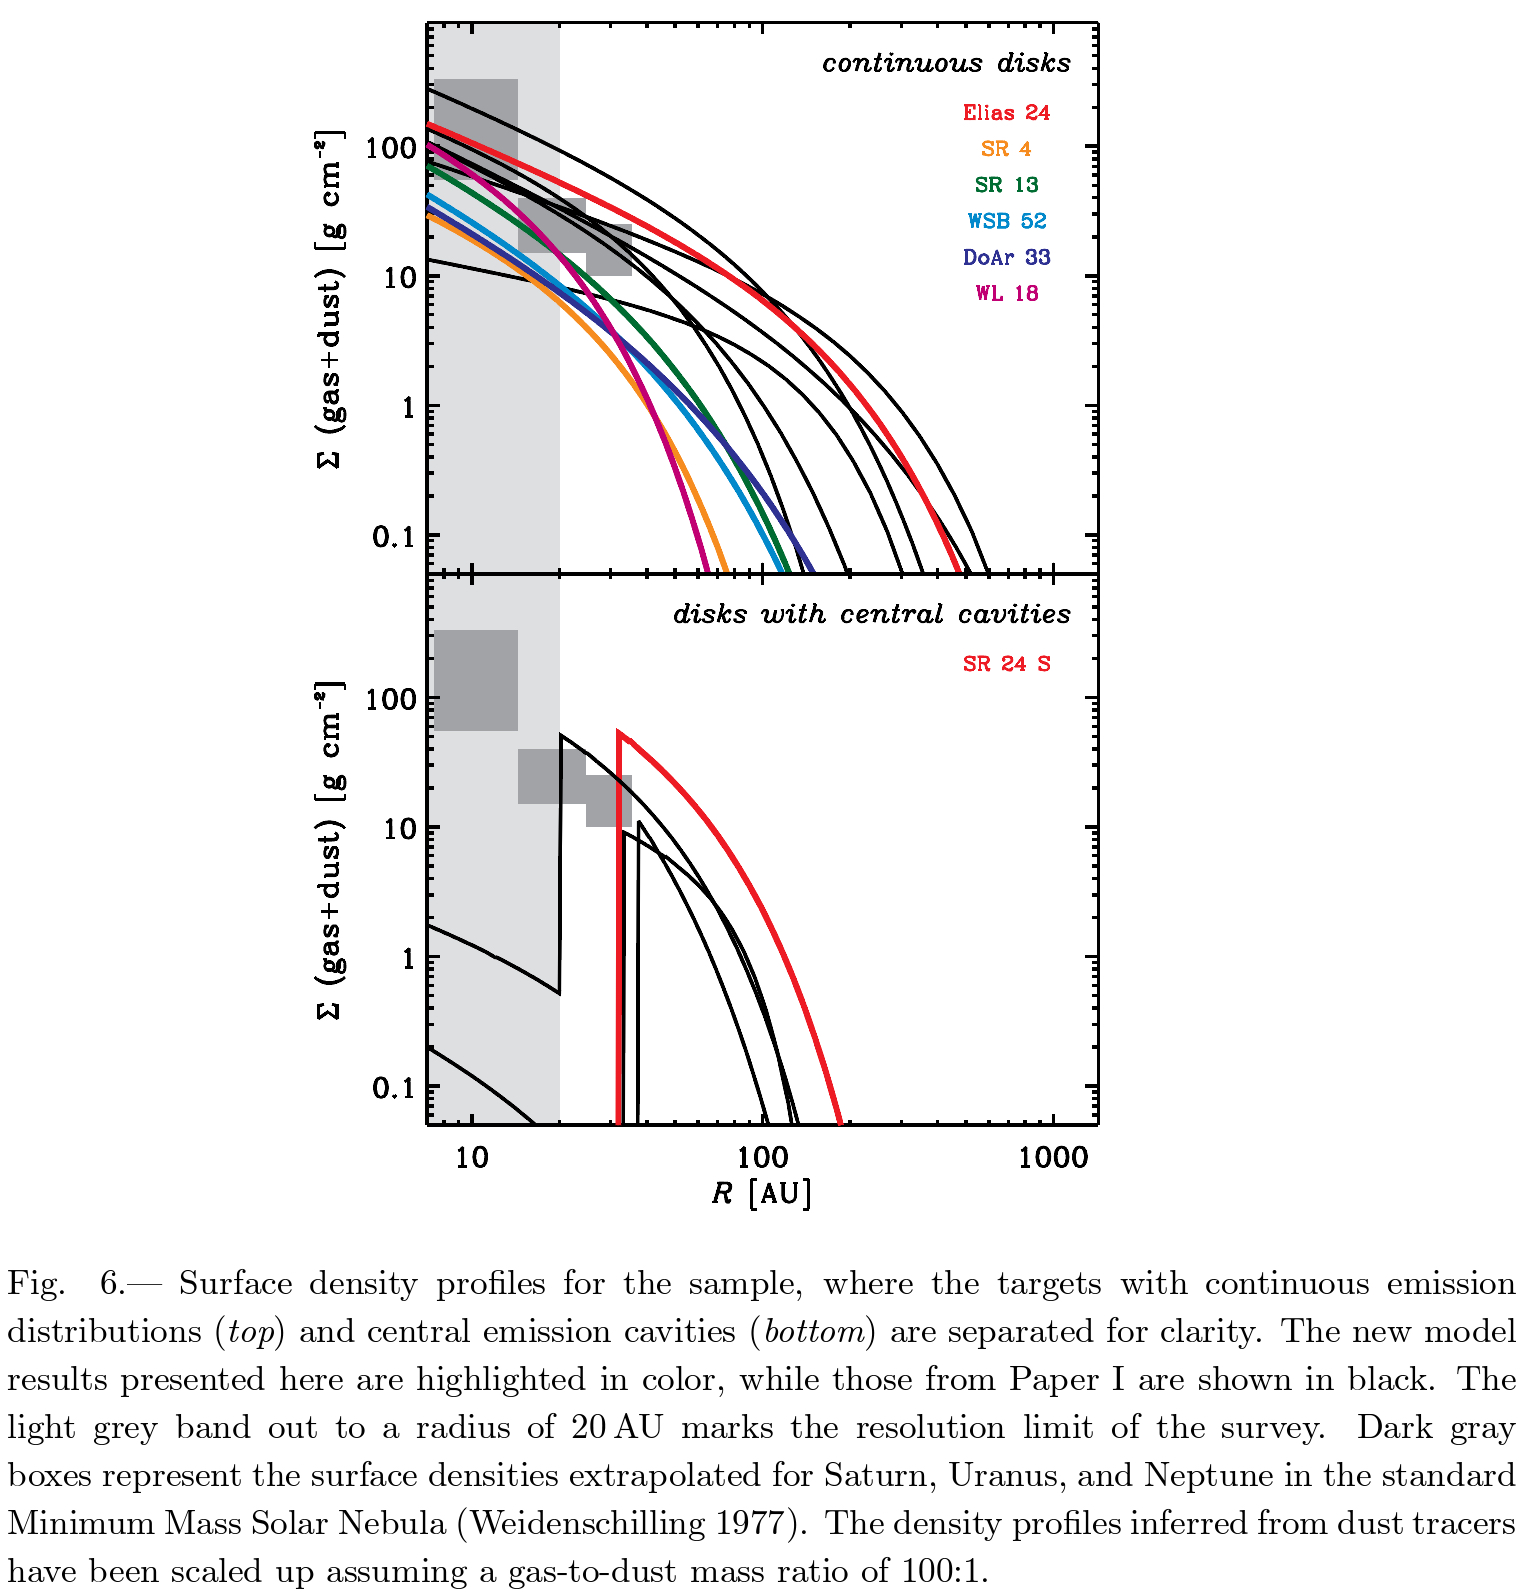
\includegraphics[trim={0cm 15cm 0 0},clip, keepaspectratio,width=0.98\textwidth]{diskdensity}
		\caption{Densit\'a superficiale dischi protoplanetari osservati nella regione di Ophiuchus ricavata risolvendo modello disco di accrescimento che riproduca densit\'a spettrale di energia osservata e il flusso a \SI{880}{\micro\meter}. I rettangoli grigi indicano densit\'a superficiale per la MMSN nella regione di Saturno, Urano e Nettuno. Da \cite{andrews2010protoplanetary}.}\label{fig:diskdensity}
	\end{subfigure}
\end{figure}

\cite{andrews2010protoplanetary} hanno osservato lo spettro emesso da oggetti nella regione di formazione stellare Ophiuchus determinando massa, dimensioni caratteristiche e viscosit\'a: $M_d=0.004-0.143\msun{}$, $\gamma=0.4-1.1$, $R_c=\SIrange{14}{198}{\astronomicalunit}$.
La figura (\subref{fig:SED-contours}) mostra le strutture attorno a stelle giovani del cluster Ophiuchus (et\'a $\tau\approx\SI{1}{\mega\year}$) secondo profili di intensit\'a a \SI{880}{\micro\meter}.
%Se $\nu\propto r\expy{\gamma}$ una soluzione di \eqref{eq:sigmaevol} per $t=0$ \'e
%\begin{equation}
%\Sigma=(2-\gamma)\frac{M_d}{2\pi R_c^2}(\frac{r}{R_c})\expy{-\gamma}\Exp{-(\frac{r}{R_c})\expy{2-\gamma}}
%\end{equation}


\begin{wrapfigure}[6]{l}{0.5\textwidth}
	\centering
	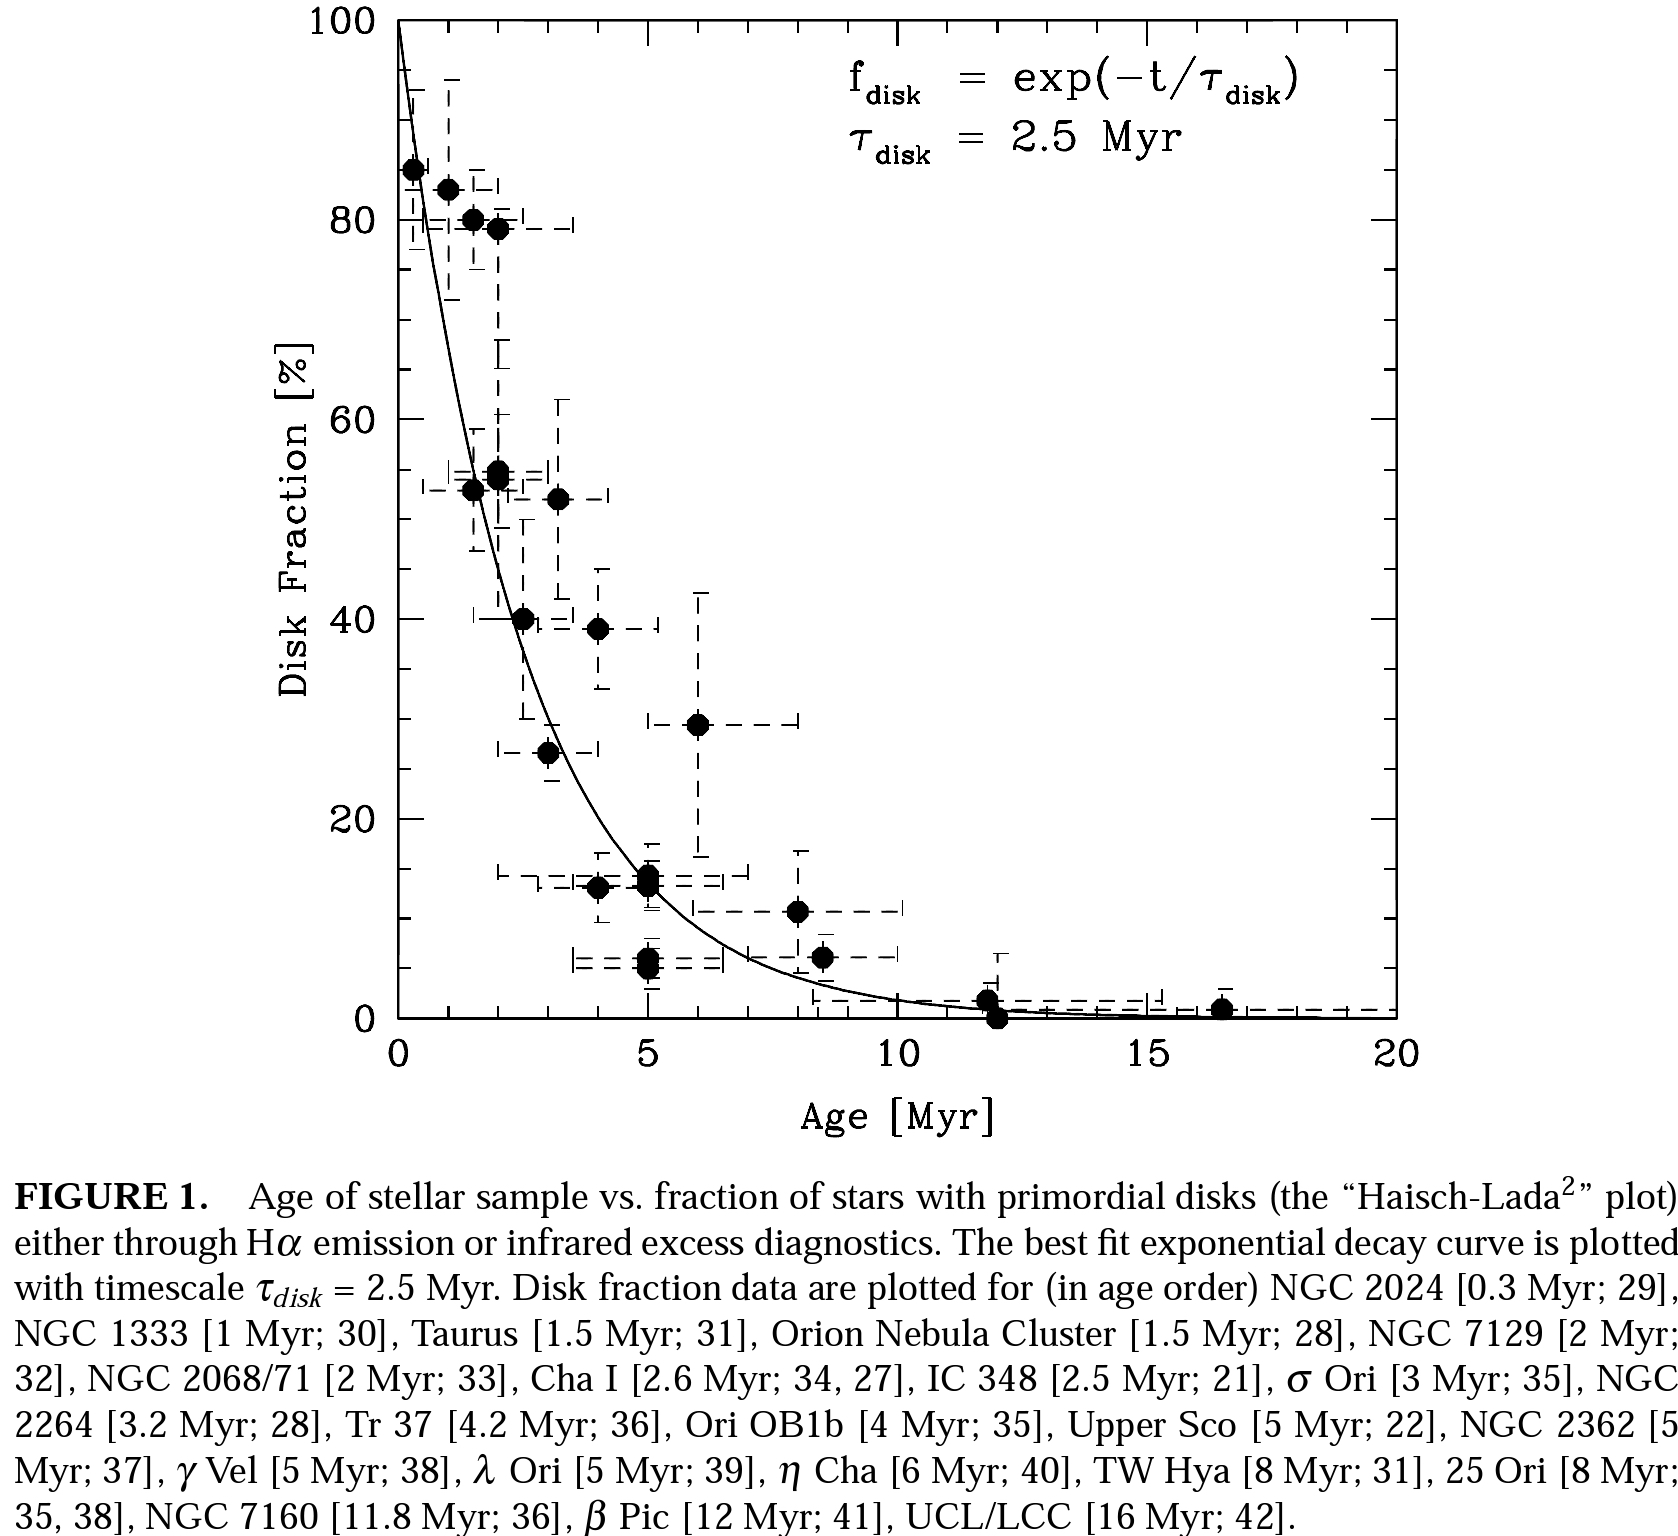
\includegraphics[trim={0cm 13cm 0 0},clip, width=0.49\textwidth,keepaspectratio]{clusterage-fstar}
	\caption{Frazione di stelle con disco protoplanetario in funzione dell'et\'a del cluster. Da \cite{mamajek2009initial}. }\label{fig:clusterage-fstar}
\end{wrapfigure}

In figura (\ref{fig:clusterage-fstar}) \'e riportata la frazione di stelle con dischi protoplanetari in funzione dell'et\'a del cluster: l'andamento \'e esponenzialmente decrescente con $\tau_c\approx\SI{2.5}{\mega\year}$.
%(\cite{haisch2001disk}) hanno determinato $\tau_c\approx\SI{6}{\mega\year}$.

%La distribuzione di massa e la frazione di dischi protoplanetari per ammassi stellari di et\'a diversa \'e mostrata in figura (\ref{fig:initdistro}). La massa \'e determinata misurando il flusso di emissione termica della polvere: la distribuzione di $\log{M_{disk}}$  \'e gaussiana e per il cluster Ophiuchus la distribuzione \'e fittata da gaussiana corrispondente a massa media $M_{disk}=0.042\msun{}$.

\begin{workout}[Disk structure: exists also temperature profile]
	Local hydrostatic equilibrium (vertical structure)
	\begin{equation}
	\frac{1}{\rho}\PDy{z}{P}=-\Omega^2z
	\end{equation}
	energy equation (energy produced by viscosity is removed by radiative flux)(ruden lin 86), optically thick medium radiative flux
	\begin{equation}
	F=-\frac{16\pi\sigma T^3}{3\kappa\rho}\PDy{z}{T}
	\end{equation}
	set of 3 ode and boundary conditions (Papa terquem 99)
	\begin{align}
	&P_s=\frac{\Omega^2H\tau_{ab}}{\kappa_s}\\
	&F_s=\frac{3}{8\pi}\dot{M}_*\Omega^2\\
	&2\sigma(T_s^4-T_b^4)-\frac{\alpha kT_s\Omega}{8\mu m_H\kappa_s}-\frac{3}{8\pi}\dot{M}_*\Omega^2=0\\
	&F(z=0)=0
	\end{align}
	s refers to $z=H$ $\tau_{ab}$ optical depth between surface and infinity, $T_b$ background T, $\mu$ mean molecular mass, $\dot{M}_*=3\pi\nu_{eff}\Sigma$.
	effect of irradiation of central star $T_s^4=T_{s,noirr}^4+T_{s,irr}^4$
\end{workout}

%\begin{tikzpicture}	
%\begin{loglogaxis}[
%xmode=log,
%log ticks with fixed point,
%	xmin=0.1, xmax=10
%	]
%\addplot gnuplot[] {10^3*1/x*(2^(-2.5+1))*exp(-x^(2-1)/1)};
%\end{loglogaxis}
%\end{tikzpicture}

\begin{workout}[Steady state solution: far from boundaries]
	Armitage lecture notes pg 19: steady state $\PDof{t}=0$
	\begin{align*}
	&\Sigma r^3\Omega v_r=\nu\Sigma r^3\TDy{r}{\Omega}+\const{}\\
	&\dot{M}=-2\pi r\Sigma v_r\\
	&-r^2\Omega\frac{\dot{M}}{2\pi}=\nu\Sigma r^3\TDy{r}{\Omega}+\const{}
	\end{align*}
	Usually determined at inner boundary: $\TDy{r}{\Omega}=0$ la costante \'e proporzionale al flusso di momento angolare $\dot{M}r^2\Omega$ (supposing disk estends to equator of slowly rotating star $\nu\Sigma=\frac{\dot{M}}{3\pi}(1-\sqrt{\frac{r_*}{r}})$)
\end{workout}

\begin{errata}[Strutture attorno a stelle giovani]
	Attorno alle stelle giovani sovente si trovano strutture opache nel visibile ma otticamente sottili nelle onde infrarosse: risolvendo il modello di disco protoplanetario, avente come input la distribuzione della dimensione della polvere e rapporto gas/polvere, per riprodurre le caratteristiche spettrali e flusso termico osservati, note anche le caratteristiche della stella centrale, si determinano i parametri caratteristici del disco.
\end{errata}

\begin{workout}[viscosit\'a disco]
	Nella popolazione planetaria simulata $\alpha$ \'e fissato sulla base delle osservazioni  ed \'e omogeneo e costante.
\end{workout}

\begin{workout}[Modello di disco di accrescimento - (Mordasini18: 4) - Introduzione descrizione fenomeni grazie a PPS]
	Refs: garaud lin 07, chiang goldreich 97
	Un modello di disco  di accrescimento usato nelle simulazioni considera l'evoluzione della densit\'a superficiale tramite l'equazione \eqref{eq:diskaccrphev-m18}
	\begin{align}
	&\TDy{t}{\Sigma}=\frac{1}{r}\PDof{r}[3r\expy{1/2}\PDof{r}(\nu\Sigma r\expy{1/2})]+\dot{\Sigma}_w(r)+\dot{\Sigma}_p(r)\label{eq:diskaccrphev-m18}\\
	&\dot{\Sigma}_w(a)=\left\{\begin{array}{c}0\\\frac{\dot{M}_w}{2\pi(a_{max}-R_g)a}\\\end{array}\right.
	\end{align}
	Densit\'a superficiale iniziale:
	\begin{equation}
	\Sigma(a,t=0)=\Sigma_0(\frac{r}{1AU})\expy{p_g}\Exp{[-(\frac{r}{R_o})\expy{2+p_g}]}(1-\sqrt{\frac{r}{R_i}})
	\end{equation}
	4-Mordasini18 (Hayashi81). $p_g\approx1$ (Andrews10).
\end{workout}

{\let\clearpage\relax\let\cleardoublepage\relax
\chapter{Caratteristiche della popolazione di esopianeti osservati}
}

\begin{wrapfigure}[10]{l}{0.65\textwidth}
	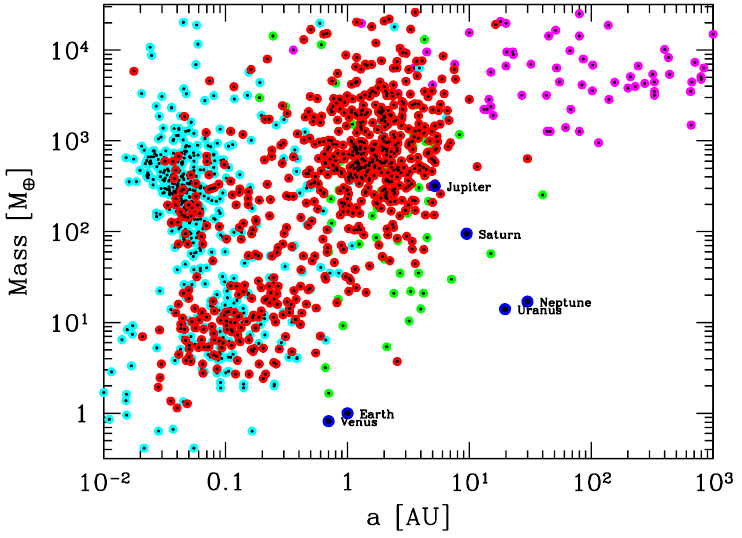
\includegraphics[trim={0cm 0 0 0},clip, width=0.65\textwidth]{obsMa}
	\caption{Diagramma massa-distanza degli esopianeti in ''The extrasolar planet encyclopedia''. Rosso, celeste, magenta e verde sono pianeti rivelati tramite RV, T, osservazione diretta e microlensing. Da \cite{mordasini2018planetary}.}\label{fig:Maplot}
\end{wrapfigure}

Il miglioramento delle capacit\'a osservative ha permesso l'osservazione di migliaia di esopianeti (vedi \cite{schneider2011defining} per una lista aggiornata): la distribuzione dei pianeti nel diagramma $a-M_p$ rappresenta la variet\'a della popolazione planetaria osservata. Per un confronto con modello di formazione planetaria \'e necessario correggere, in maniera statistica, i bias osservativi dovuti alla tecnica usata per rivelare il pianeta, alle caratteristiche dello strumento e della stella che lo ospita. Adesso considero le caratteristiche dei pianeti come risultano da survey che usano le tecniche di velocit\'a radiale e transito.

\section{Popolazione esopianeti rilevati tramite velocit\'a radiale}

Considero il moto stellare attorno al centro di massa del sistema stella pianeta:
se l'asse z \'e lungo la linea di vista la posizione della stella \'e $z=r(t)\sin{i}\sin{(\omega+\nu)}$ e per la velocit\'a radiale:
\begin{equation}
v_r=\dot{z}=K[\cos{(\omega+\nu)}+e\cos{\omega}]\label{eq:vrsignal}
\end{equation}
\begin{equation}
K=\frac{2\pi}{P}\frac{a_*\sin{i}}{(1-e^2)\expy{1/2}}=\frac{\SI{28.4}{\meter\per\second}}{\sqrt{1-e^2}}(\frac{M_p\sin{i}}{M_J})(\frac{P}{\si{\year}})\expy{-1/3}(\frac{M_*}{\msun})\expy{-2/3}
\end{equation}
%K=(\frac{2\pi G}{P})\expy{1/3}\frac{M_p\sin{i}}{(M_p+M_*)\expy{2/3}}\frac{1}{(1-e^2)\expy{1/2}}
dove $K$ \'e la semi-ampiezza.
Un numero di misure della velocit\'a radiale permettono di determinare alcuni parametri orbitali ($e$, $P$, $t_p$, $\omega$) e la massa minima $M_p\sin{i}$. In (\cite{cumming2004detectability}) sono riportati i valori soglia del rapporto signale rumore per avere probabilit\'a rivelamento pianeta al $50\%$ o $99\%$ in funzione del setup osservativo.

\begin{workout}[Detection probability - Global efficiency]
Per probabilit\'a di rivelamento del $50\%$ la minima massa planetaria \'e
\begin{equation}
M_{p,min}\approx4\mearth{}(\frac{N}{20})\expy{-1/2}(\frac{\sigma}{\SI{1}{\meter\per\second}})(\frac{P}{\SI{1}{\day}})\expy{1/3}(\frac{M_*}{\msun{}})\expy{2/3}
\end{equation}
dove $\sigma$ tiene conto errori strumentali e rumore stellare.
Global efficiency of doppler measurement in given survey
This efficiency include precision of spectrograph, sample star characteristics and observing strategy (measurement frequency, exposure time long enough to diminish intrinsic stellar noise and photon noise).
cumming 2004/08
precisione strumentale:
rapporto segnale rumore $K/s$ per avere probabilit\'a di rivelazione $50/99\%$.
\end{workout}
Per sistemi multipli si considera la sovrapposizione lineare di $n_p$ termini \eqref{eq:vrsignal}: viene sottratto il segnale Kepleriano dominante fino a che resta solo rumore.

La probabilit\'a di rivelamento di un pianeta che orbita attorno a stella con date caratteristiche \'e determinata dall'ampiezza del moto radiale della stella attorno al centro di massa K, il rumore strumentale e stellare, la durata dell'osservazione e la forma dell'orbita del pianeta.
Riporto i risultati del survey HARPS+CORALIE (\cite{mayor2011harps}), capace di rivelare giganti gassosi entro $P<\SI{12}{\year}$ e super Terre/pianeti nettuniani con $P<\SI{100}{\day}$.

\begin{workout}[ricopiare risultati mayor11]
	?
\end{workout}

\begin{figure}[!ht]
\centering
\begin{subfigure}[b]{0.4\textwidth}
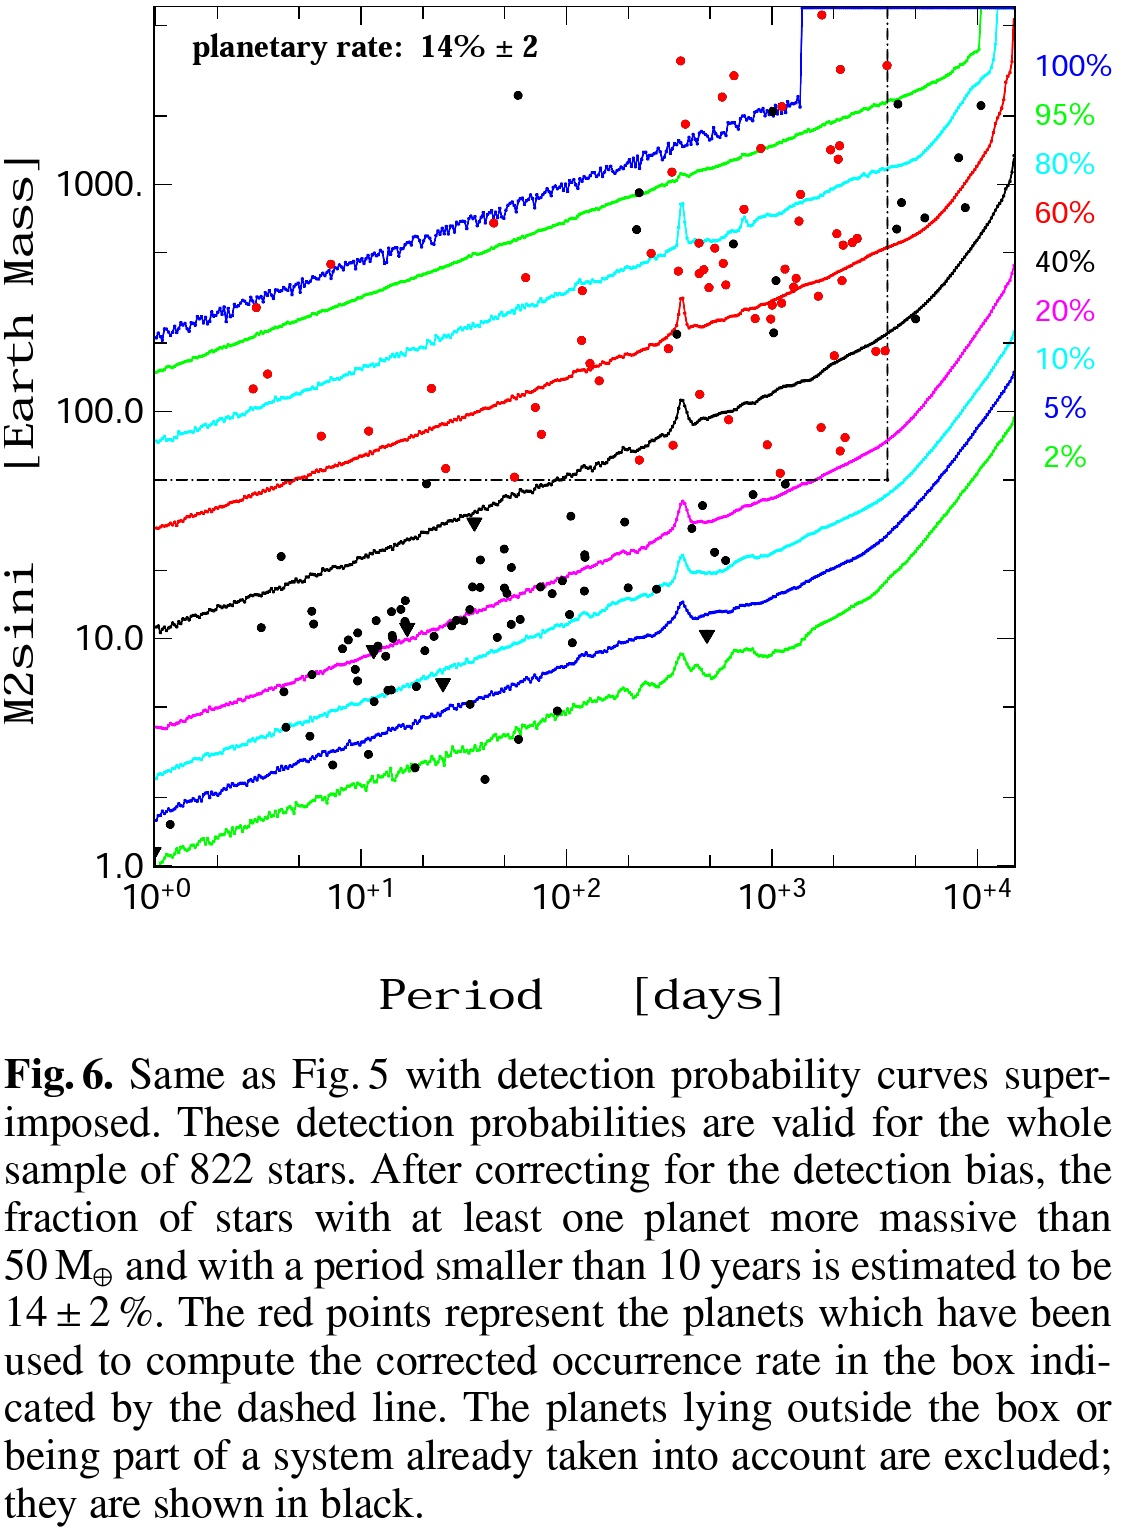
\includegraphics[trim={0cm 17cm 1cm 0},clip, width=0.99\textwidth]{PMfreq-e23}\label{fig:PMfreq-e23}
\end{subfigure}
~
\begin{subfigure}[b]{0.4\textwidth}
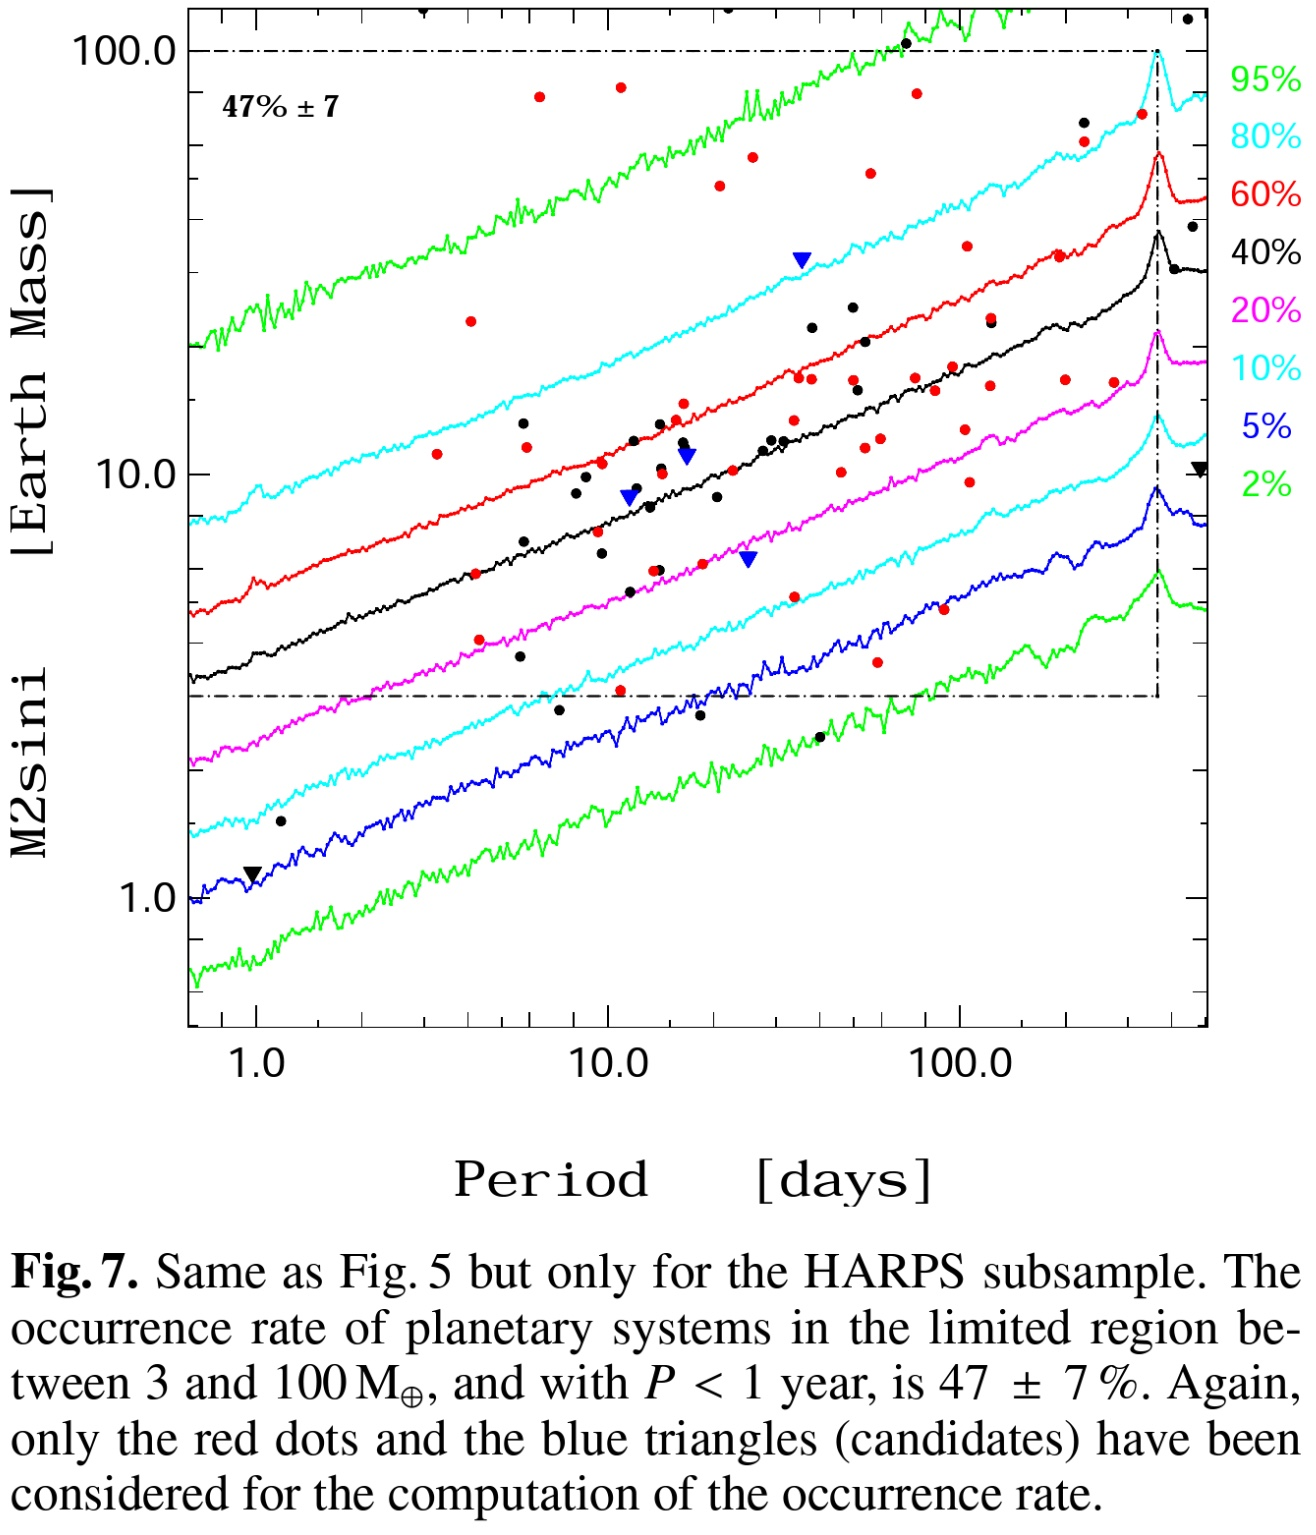
\includegraphics[trim={0cm 10cm 0 0},clip, width=0.99\textwidth]{PMfreq-e12}\label{fig:PMfreq-e12}
\end{subfigure}%

\begin{subfigure}[b]{0.4\textwidth}
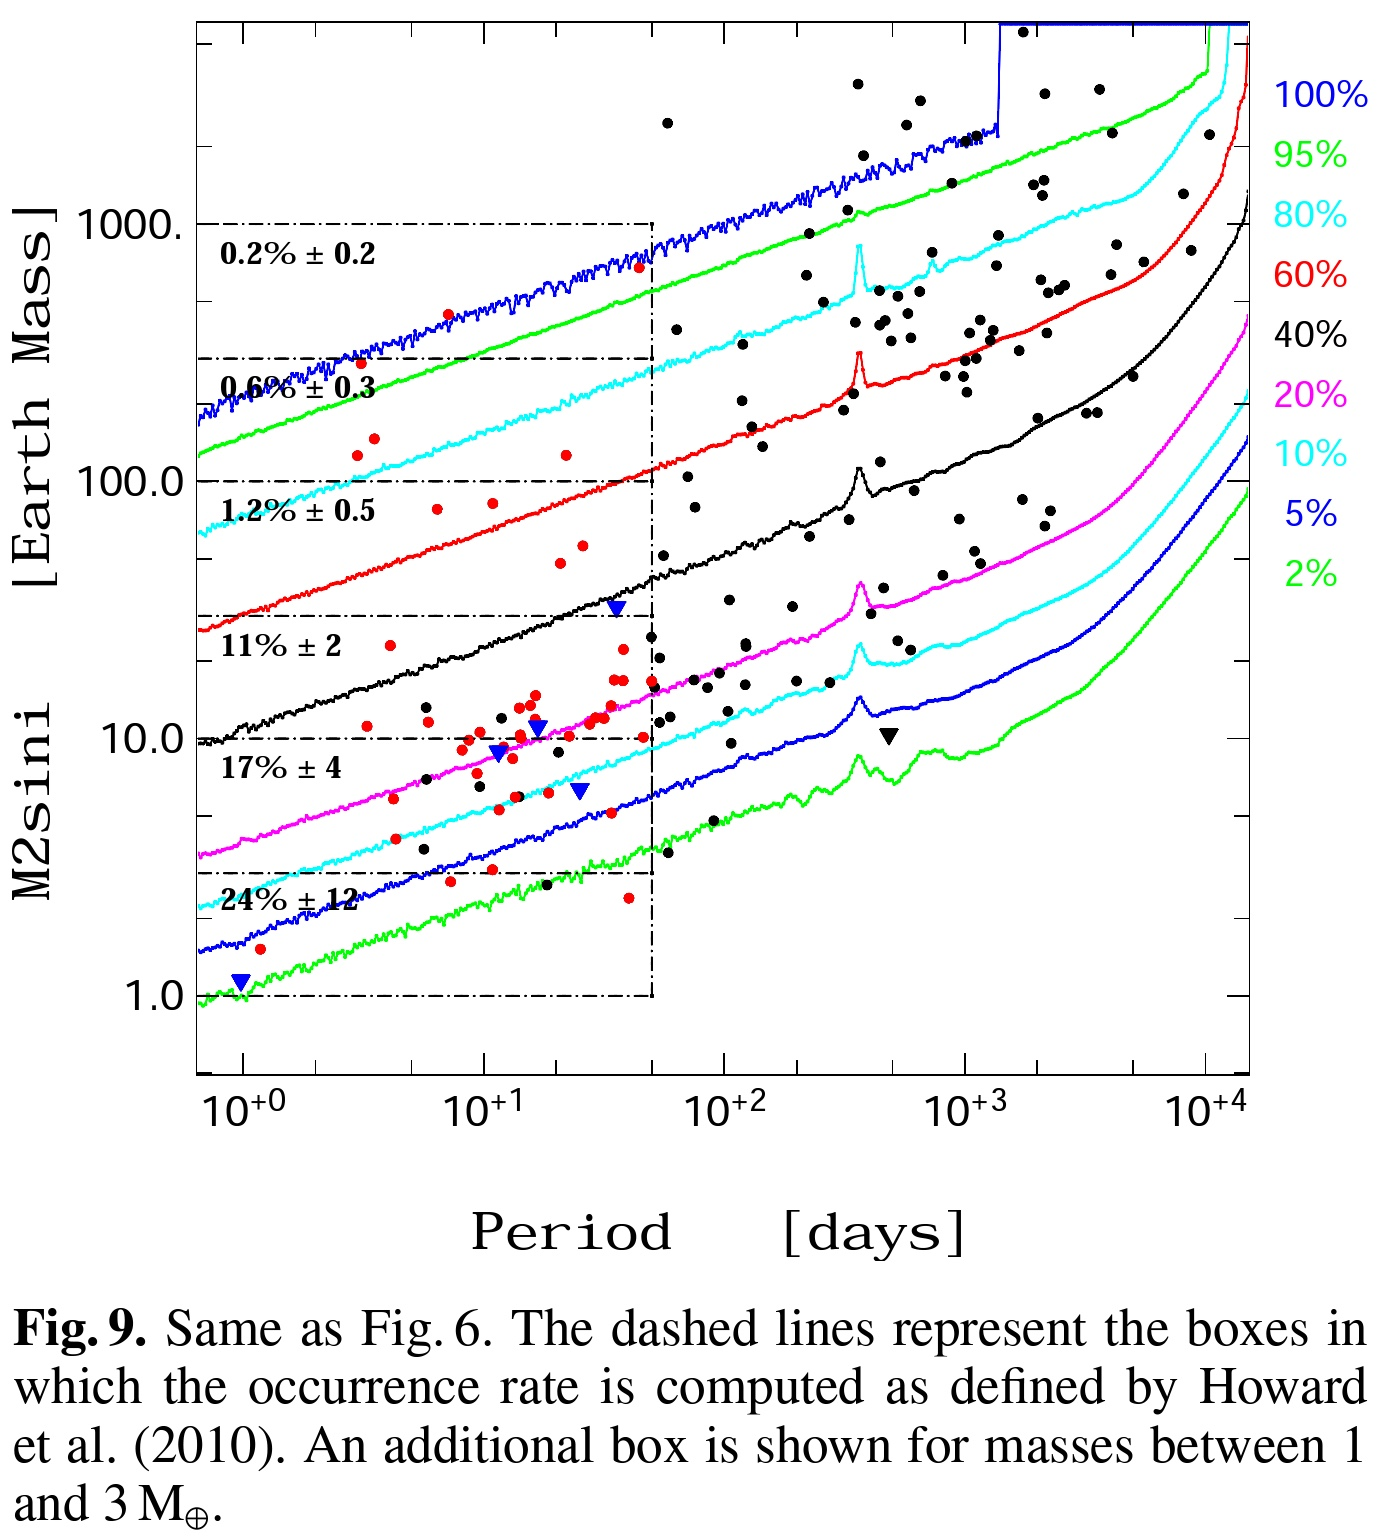
\includegraphics[trim={0cm 8cm 0 0},clip, width=0.99\textwidth]{PMfreq-short}\label{fig:PMfreq-short}
\end{subfigure}
\caption{Diagramma massa-periodo: frazione di stelle che ospitano pianeta con caratteristiche nella regione evidenziata corretta per bias osservativi. Da sinistra a destra: $P<10\si{\year}$ e $M>50\mearth{}$, $P<1\si{\year}$ e $M>3-100\mearth{}$, $P<50\si{\day}$ e $M=1-3/3-10/10-30/30-100/100-300/300-1000$. Da \cite{mayor2011harps}.}\label{fig:PMfreqs}
\end{figure}

\begin{workout}[rileggere l'articolo mayor 11: harps neptunian etc]
risultati e pianeti abitabili
\end{workout}

I tre diagrammi (\ref{fig:PMfreqs}) mostrano la frequenza dei pianeti in delimitate regioni del diagramma periodo-massa ($P-M$) determinata utilizzando un sottocampione di stelle per cui la probabilit\'a di rivelazione relativa alla regione del diagramma $(P-M)$ \'e $99\%$: accanto alle linee continue nei diagrammi $(P,M)$ \'e indicata la percentuale di stelle per cui \'e possibile ottenere una probabilit\'a di rivelamento del $99\%$.

\begin{figure}[!ht]
\begin{subfigure}[b]{0.49\textwidth} \centering 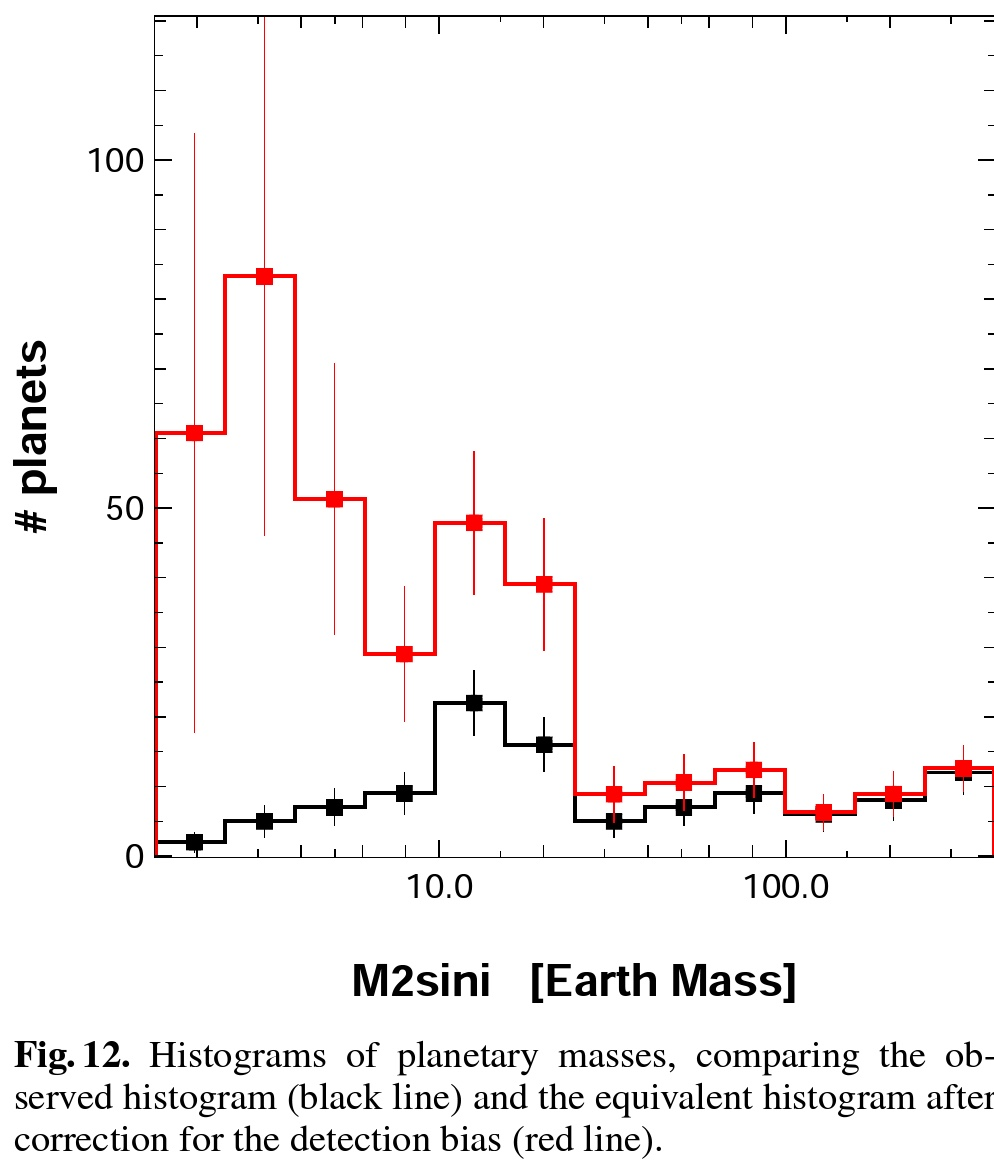
\includegraphics[trim={0cm 5cm 0 0},clip, width=0.94\textwidth]{freqvsM}
\caption{Distribuzione di massa di massa dei pianeti: in rosso distribuzione corretta per bias osservativi. Da \cite{mayor2011harps}.}\label{fig:freqvsM}
\end{subfigure}
~
\begin{subfigure}[b]{0.49\textwidth} \centering 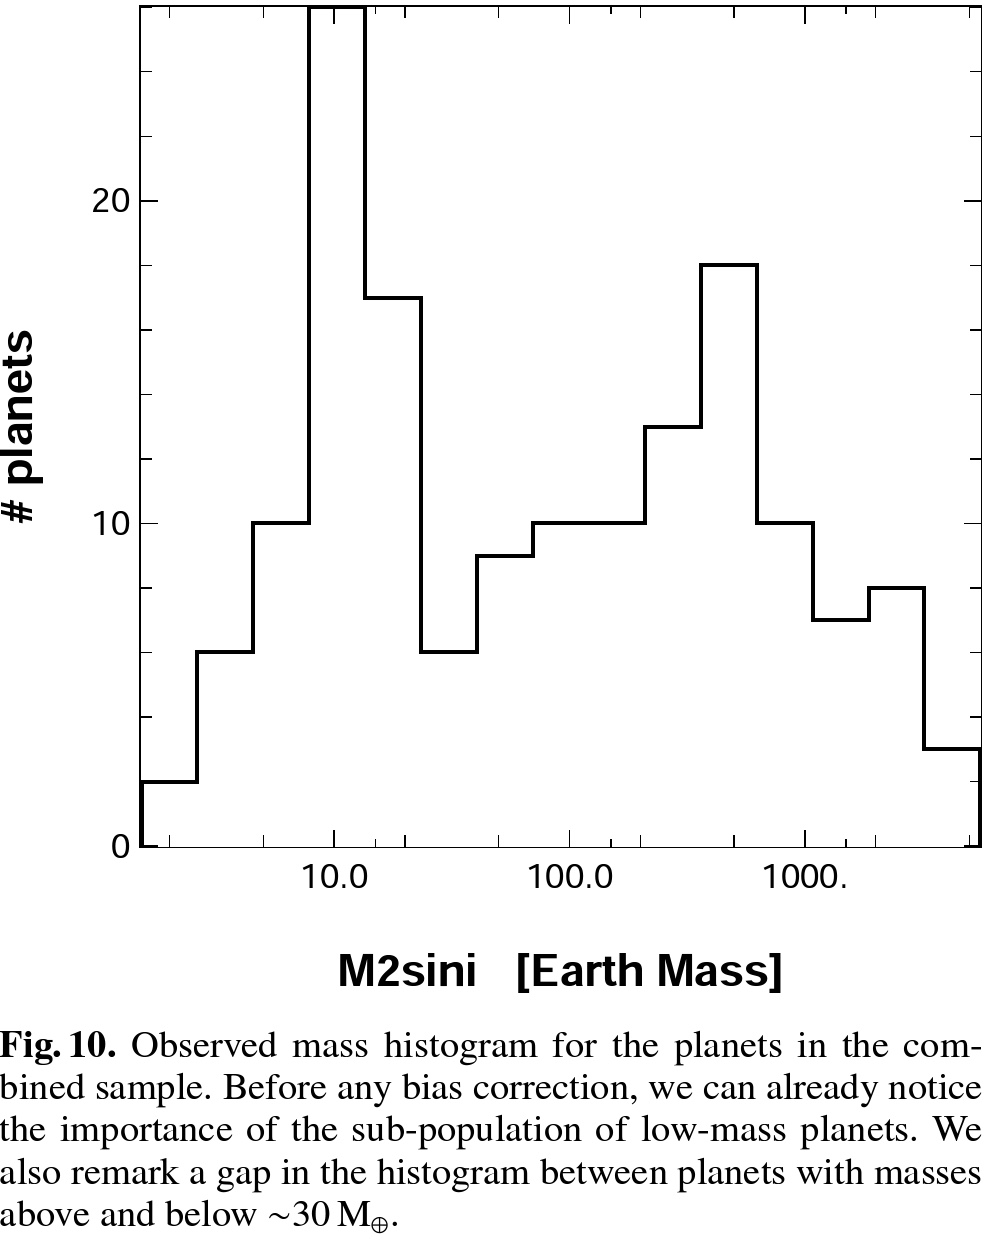
\includegraphics[trim={0cm 8cm 0 0},clip, width=0.94\textwidth]{freqvsMcomb}
\caption{Distribuzione di massa dei pianeti osservata. Da \cite{mayor2011harps}.}\label{fig:freqvsMcomb}
\end{subfigure}
\end{figure}

\begin{figure}[!ht]
\centering 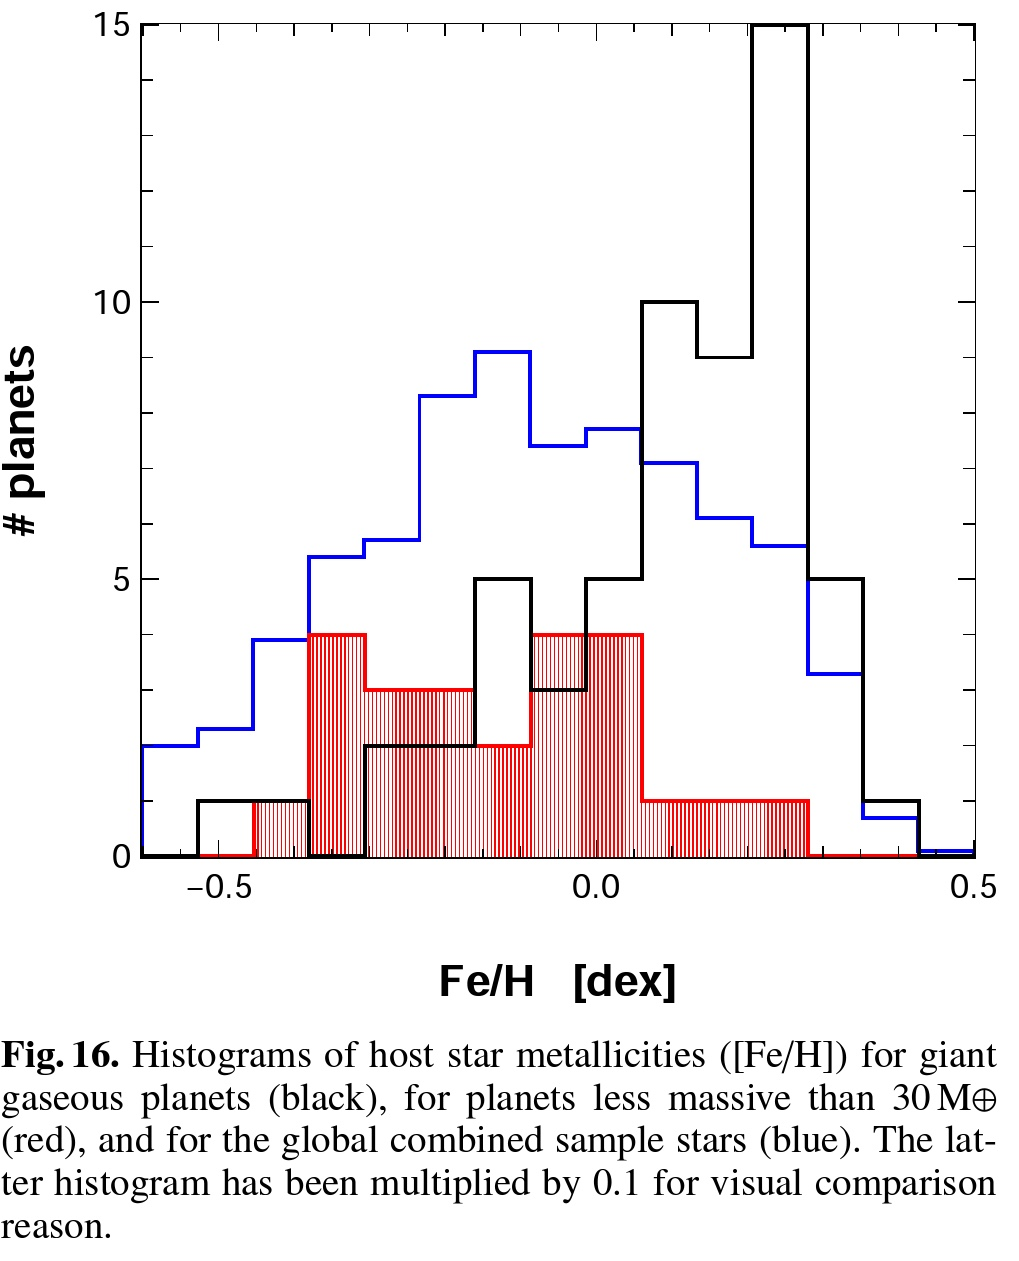
\includegraphics[trim={0cm 8cm 0 0},clip, width=0.43\textwidth]{PfreqvsFeH}
\caption{Numero di pianeti in funzione della metallicit\'a stellare: nero dei giganti gassosi, rosso dei pianeti con $M\leq30\mearth{}$ e blu combinata. Da \cite{mayor2011harps}.}\label{fig:PfreqvsFeH}
\end{figure}

La distribuzione di massa (figure \subref{fig:freqvsM}, \subref{fig:freqvsMcomb}) mostra un'abbondante popolazione di pianeti di massa piccola e una rapida diminuzione attorno a $10\mearth{}$; la distribuzione dei periodi mostra aumento dei pianeti giganti ($M>30\mearth{}$) a maggiore periodo orbitale (figura \subref{fig:freqvsPgiant}) e concentrazione pianeti piccola massa a $P=10-100\si{\day}$ (figura \subref{fig:freqvsPlowM}).

La figura (\ref{fig:PfreqvsFeH}) mostra l'assenza di correlazione tra la metallicit\'a della stella e la frequenza di pianeti di piccola massa fino a $30-40\mearth{}$ al contrario di quello che accade per pianeti giganti.

\begin{figure}[!ht]
\begin{subfigure}[b]{0.49\textwidth} \centering 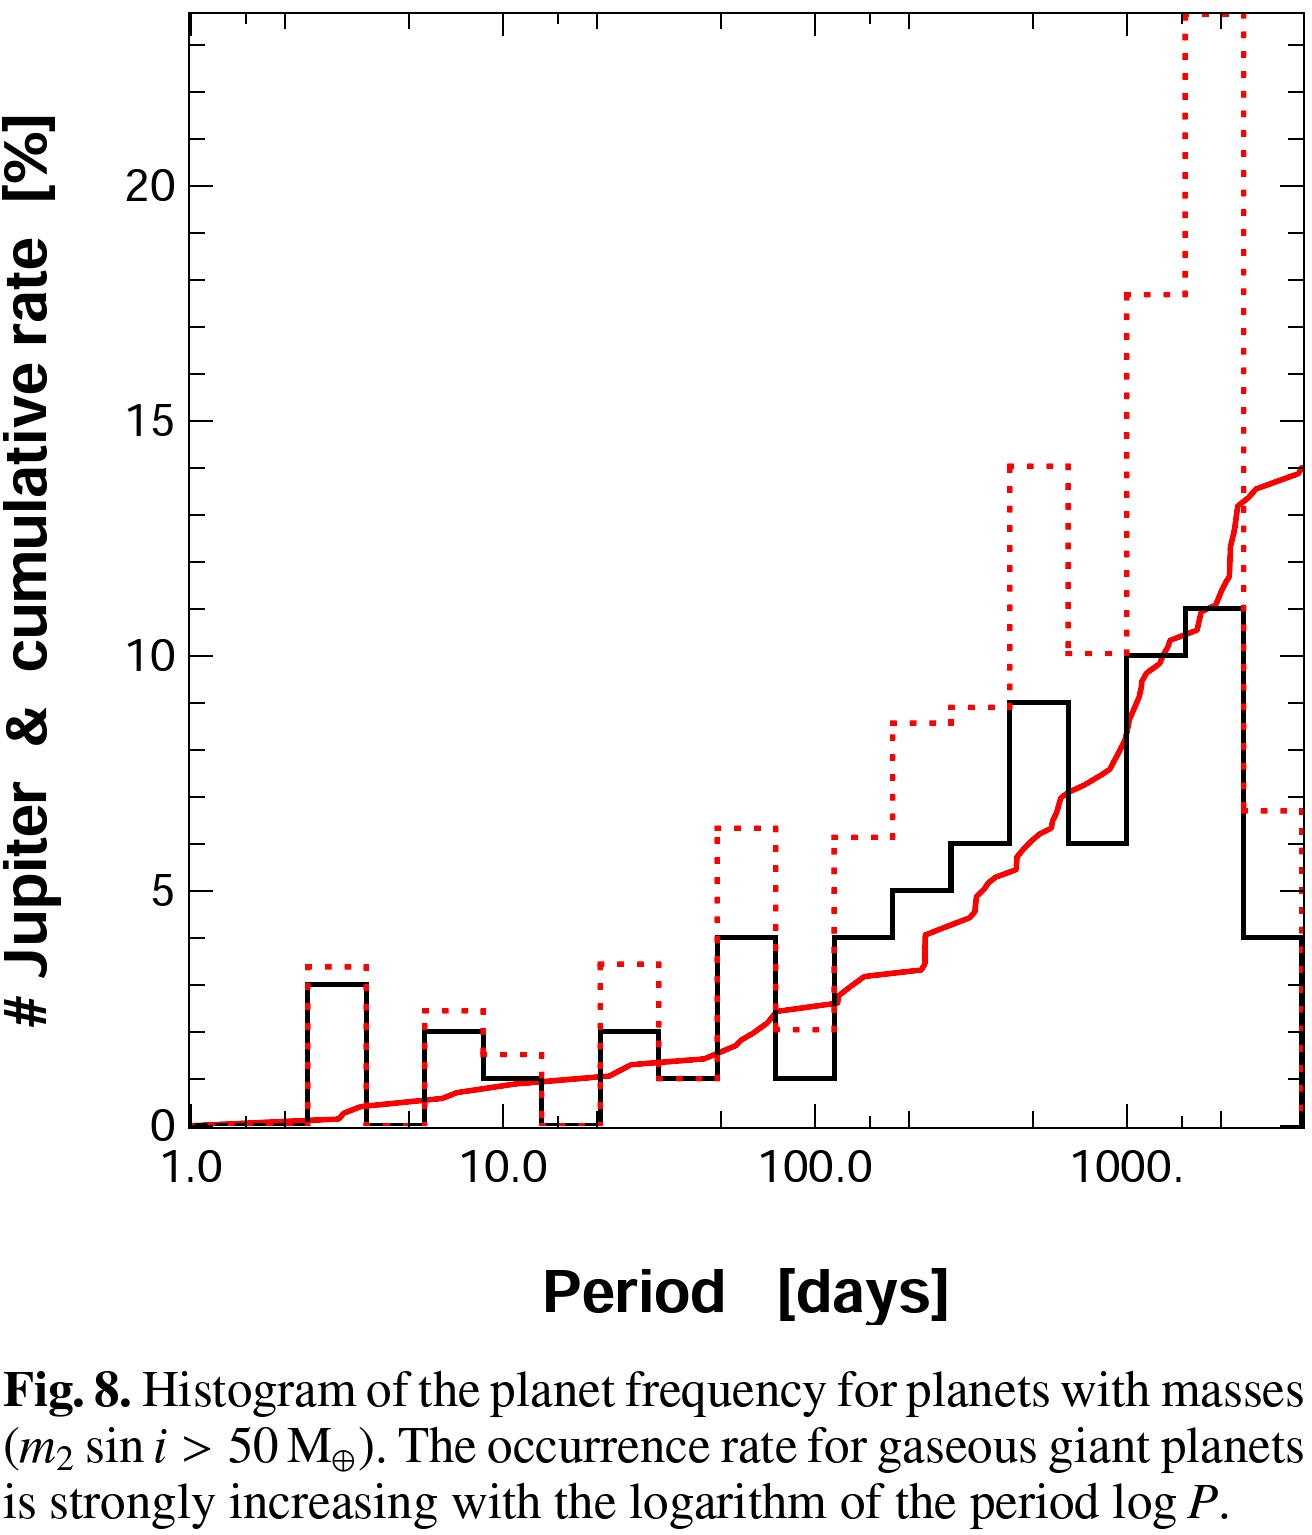
\includegraphics[trim={0cm 6cm 0 0},clip, width=0.98\textwidth]{freqvsPgiant}\caption{Frequenza pianeti con $M\geq 30\mearth{}$ in funzione del periodo orbitale; in rosso  tratteggiato con correzione bias osservativi. Da \cite{mayor2011harps}.}\label{fig:freqvsPgiant} \end{subfigure}
~
\begin{subfigure}[b]{0.49\textwidth} \centering 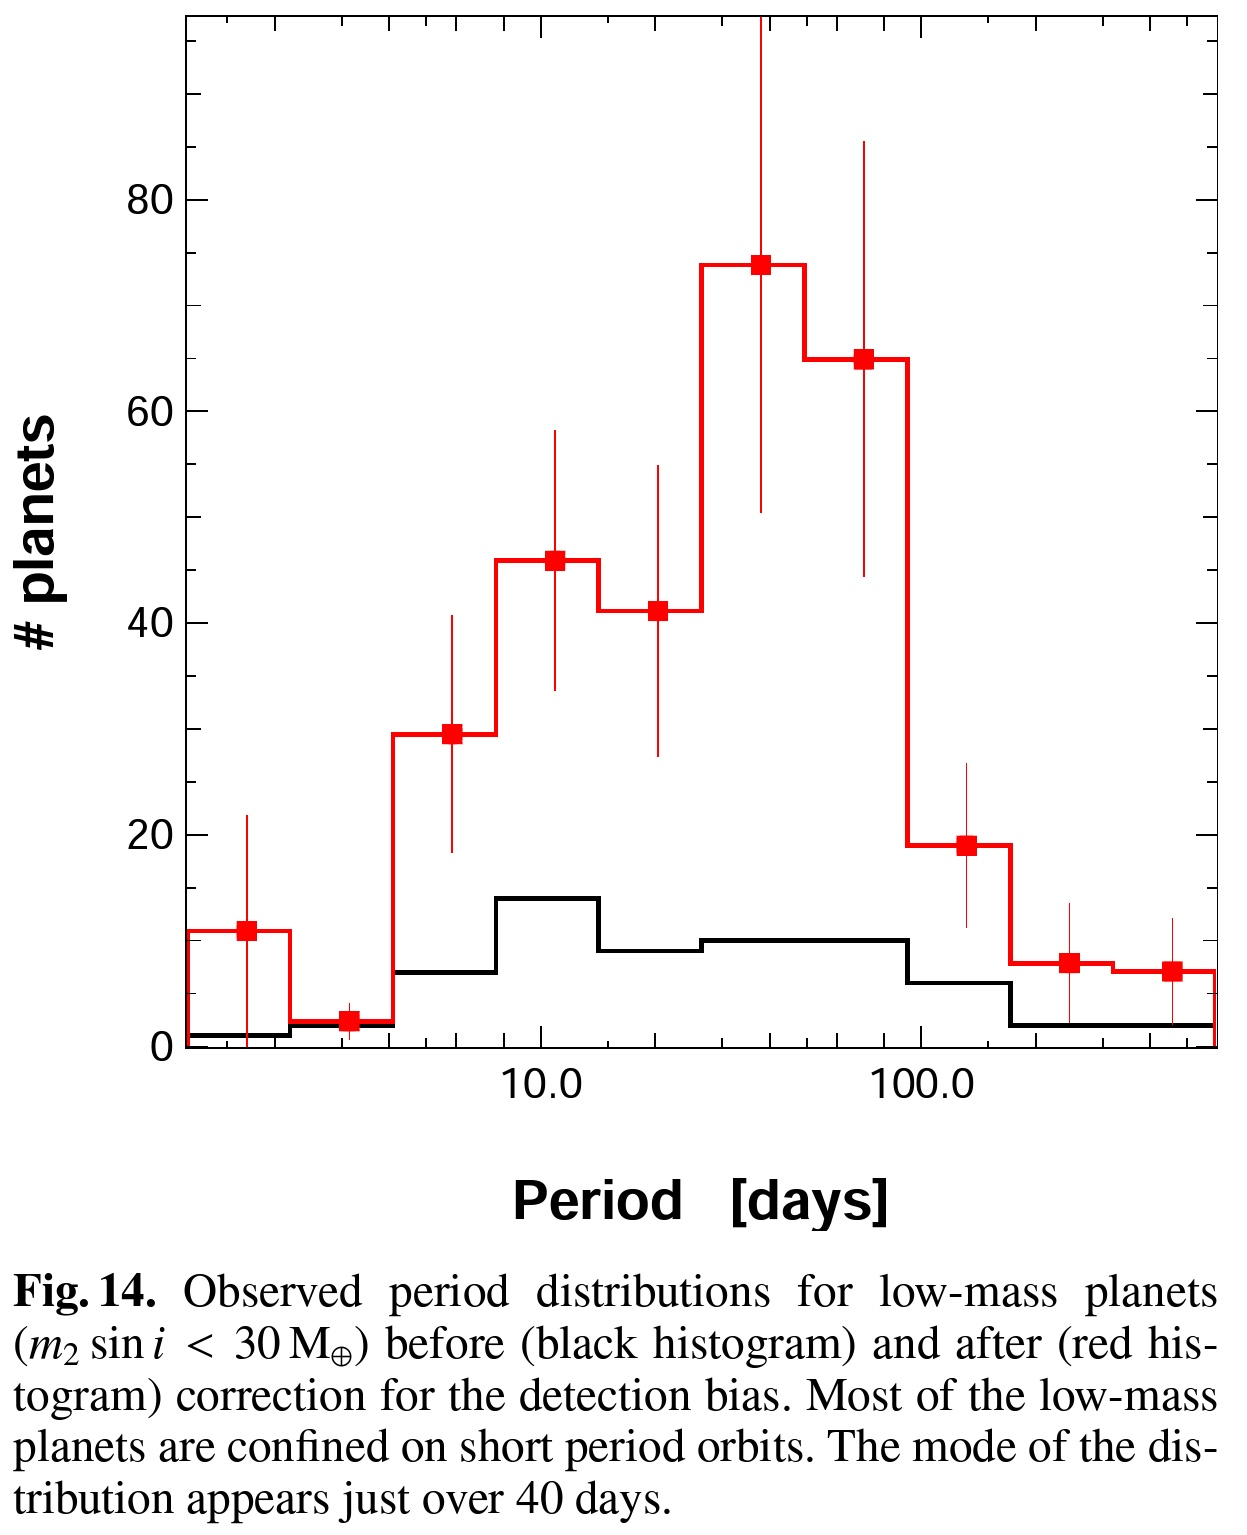
\includegraphics[trim={0cm 10cm 0 0},clip,width=0.98\textwidth]{freqvsPlowM} \caption{Frequenza pianeti con $M\leq 30\mearth{}$ in funzione del periodo orbitale; in rosso con correzione bias osservativi. Da \cite{mayor2011harps}.}\label{fig:freqvsPlowM}
\end{subfigure}
\end{figure}

\begin{workout}[Spostamento picco superterre-aumento massa pianeti giganti all'aumentare del periodo]
Una comprensione pi\'u ampia si ha studiando la distribuzione dei pianeti nel diagramma massa-periodo (M-P): elenco alcune caratteristiche della distribuzione dei pianeti osservati (da \cite{mayor2011harps}).
\begin{itemize}
\item Il picco della densit\'a di super-terre si sposta da $6\mearth{}$ a $10\mearth{}$ per periodi da \SI{10}{\day} a \SI{100}{day}
%\item Non sono osservati pianeti fino a $50\mearth{}$ con $P>\SI{1000}{\day}$
\item il pianeta gassoso pi\'u massiccio aumenta da $1\mjupiter{}$ a $15\mjupiter{}$ passando da $P\approx\SI{1}{\day}$ a $P\approx\SI{15}{\year}$.
\end{itemize}
\end{workout}


\begin{workout}[Origin of metallicity excess: stellar structure]
Pinsonneault depoy caffee 01
\end{workout}•

\begin{workout}[minimo in mass distro]
\'e un minimo? ha un significato?
\end{workout}

\begin{workout}[dtectability and selection effects (pg 14)]
Perrymann pg 34 fig 2.25 d
fig 2.6,fig 2.18
\end{workout}

\begin{workout}[multplanet system: mean motion resonances, orbital spacing,...]
dynamical classification (barnes 08): tidal dominated if ($a<0.1$), resonant dom. if one resonant argument librates, secular otherwise.
Many systems are found dyn full and stability: packed planetary system hypothesis (Barnes Quinn 04, Barnes Raymond 04, Raymond Barnes 05, Raymond 06), orbital stability for closely packed (smith lissauer 09), outer solar system is very stable and dyna full (Levinson duncan 93, inner is less stable but dyna full (sussman wisdom 92, laskar 94)
n-body integration-orbit fitting: deprojected mass and relative inclination
perryman pg 38
Interazione n-body protopianeti vs evoluzione a lungo termine: i pianeti arrivano a risonanze attraverso migrazione
Kepler: latham 11 (first comparison of kepler planet), burke 14
wright09: ten multiplanet sysytem and systematic
Winn, Fabricky 15
fig 2.30 pg 39 Perrymann
(ford rasio 08: dynamical outcomes of PP scattering)

\begin{figure}[!ht]
\begin{subfigure}[b]{0.47\textwidth}
\centering
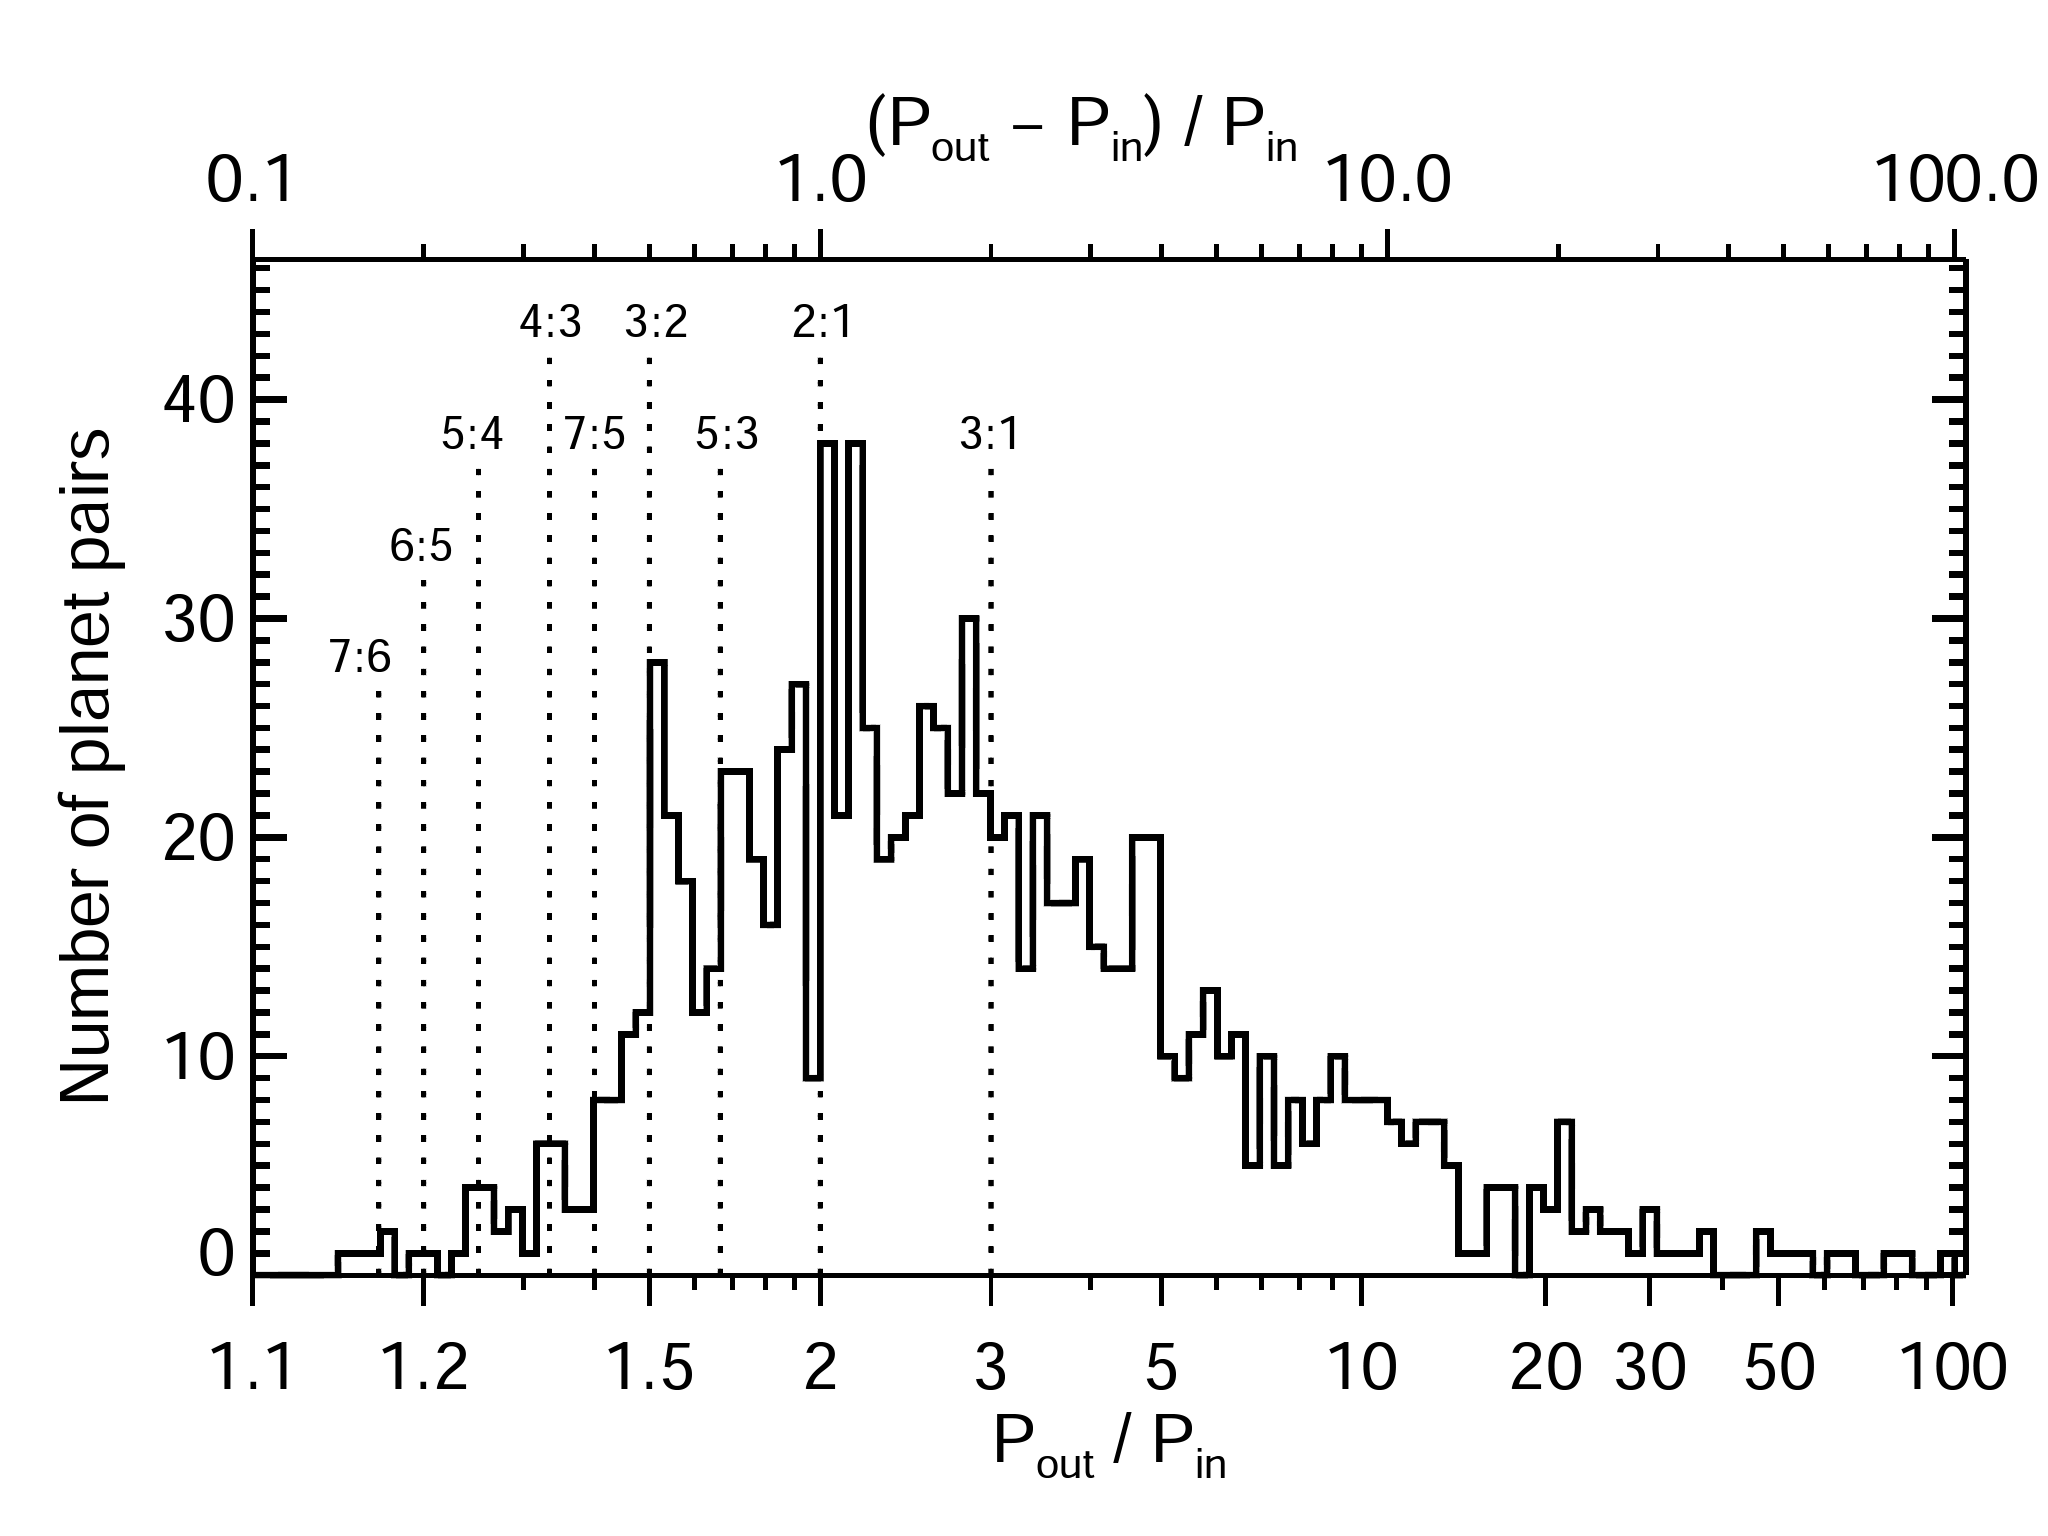
\includegraphics[trim={0cm 0 0 0},clip, width=0.9\textwidth]{exoresonance}
\caption{Da \cite{winnfabrycky15}.}\label{fig:exoresonance}
\end{subfigure}
~
\begin{subfigure}[b]{0.47\textwidth}
\centering
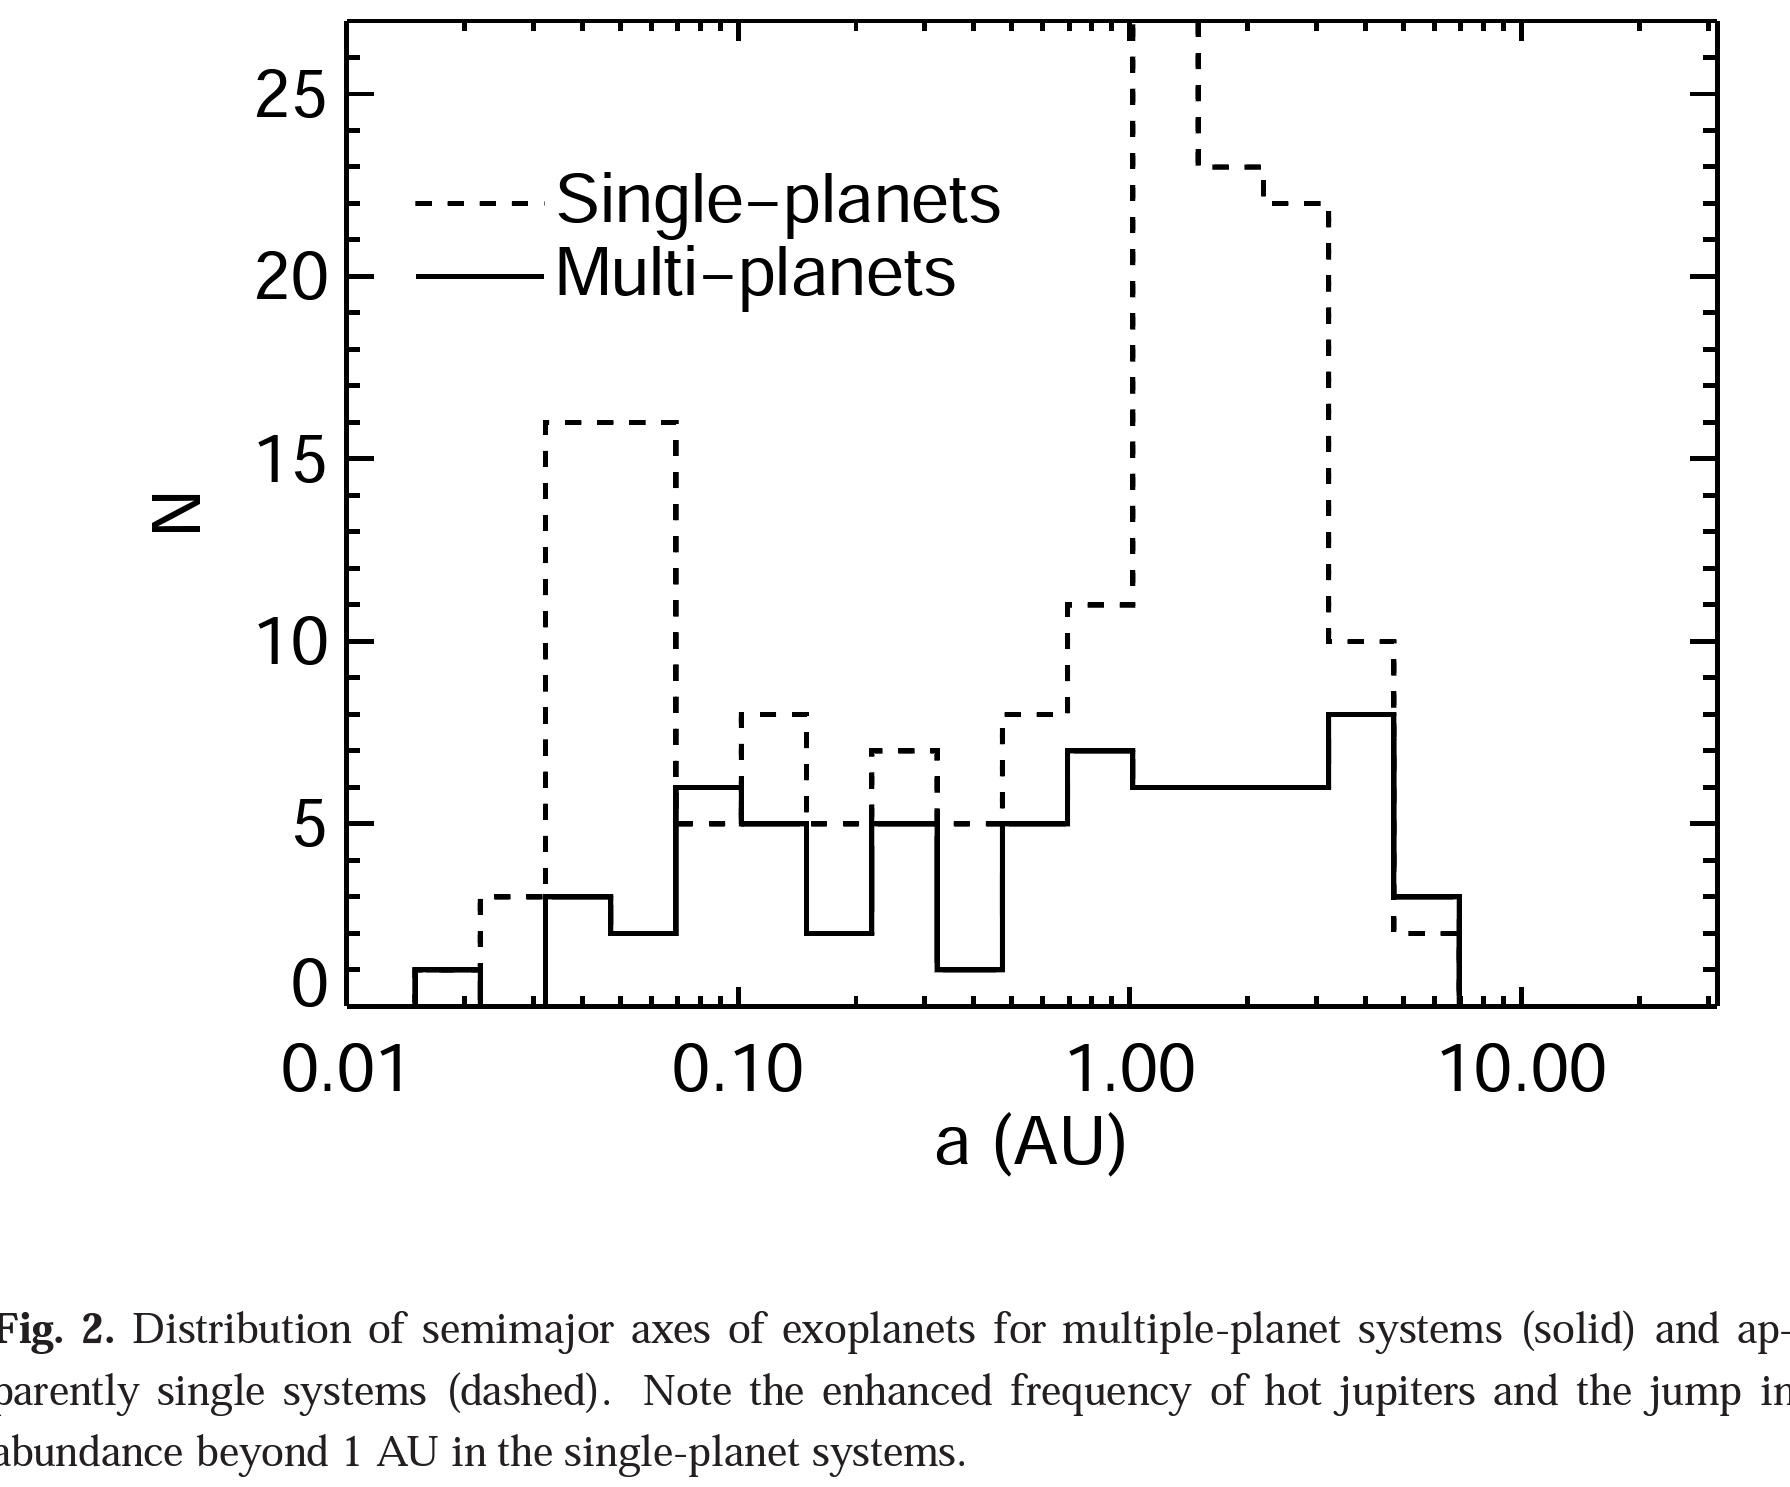
\includegraphics[trim={0cm 0 0 0},clip,width=0.9\textwidth]{singlemulti}
\caption{Da \cite{wright09}.}\label{fig:singlemulti}
\end{subfigure}
\end{figure}
\end{workout}

\begin{workout}[eccentricity distro: occurrence and architecture]
wright 09: multiplanet system tend to havelower eccentricity,
Limbach turner 14: $e_m\propto N\expy{-1.2}$.
planet around metal rich star have higher e (dawson, murray-clay 13)
smaller planets tend to have lower e (hogg 10 raccomanded modelling e distro on basis of Bayesian analysis)
\end{workout}

\clearpage

\section{Popolazione esopianeti rilevati tramite transito}

Le osservabili sono la differenza di luminosit\'a durante il transito, la durata totale e di massima occultazione del transito, e il periodo: da questi \'e possibile ricavare $R_p$, a, i, $R_*$, $M_*$ facendo uso della relazione massa raggio appropriata per la fase evolutiva della stella, per stelle di sequenza principale
\begin{equation}
\frac{R_*}{\rsun{}}=(\frac{M_*}{\msun{}})\expy{0.8}
\end{equation}

La probabilit\'a che l'orbita di un pianeta sia allineata con l'osservatore in maniera da avere un transito \'e:
\begin{equation}
p=(\frac{R_*\pm R_p}{a})(\frac{1}{1-e^2})=0.005(\frac{R_*}{\rsun{}})(\frac{a}{1AU})\expy{-1}(\frac{1}{1-e^2})
\end{equation}
dove $\pm$ indica inclusione/esclusione di transiti a raso.

Considerando un numero totale di osservazioni $N_o$ durante il transito si hanno $N_t\approx N_o\frac{R_*}{\pi a}$; il rapporto segnale rumore \'e $S/N=\sqrt{N_t}\frac{\delta}{\sigma}$, $\sigma$ precisione fotometrica e $\delta=(\frac{R_p}{R_*})^2$. Per osservazione limitata da statistica fotoni $\sigma\propto\frac{1}{\sqrt{N_{ph}}}\propto d$: fissato S/N (e tipo stellare) il numero di pianeti rivelati varia come volume a cui \'e estesa la ricerca per probabilit\'a di transito:
\begin{equation}
V_p*P\propto d^3*\frac{R_*}{a}\propto R_p^6/P\expy{\frac{5}{3}}
\end{equation}

Il grafico (\ref{fig:H12yield}) mostra i risultati del survey di ricerca di transiti attorno a stelle di tipo solare realizzato con satellite kepler: si nota un picco di densit\'a nella regione del diagramma P-R da $P\approx\SI{3}{\day}$, $R\approx2\rearth$ a $P\approx\SI{50}{\day}$, $R\approx4\rearth$.

\begin{figure}[!ht]
	\centering
	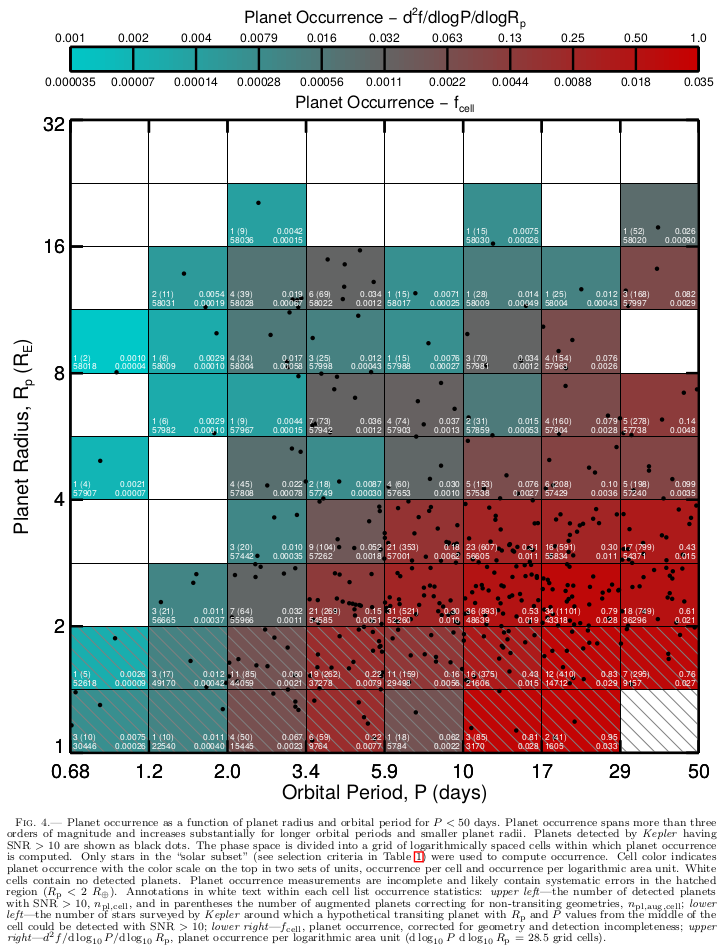
\includegraphics[trim={0cm 3.5cm 0 0},clip,width=0.95\textwidth,keepaspectratio]{H12yield}
	\caption{Frequenza pianeti osservati in funzione del raggio $R_p$ e del periodo $P$. In bianco per ogni cella \'e indicato: a sinistra in alto il numero di pianeti rivelati con SNR maggiore di una certa soglia scelta dagli autori del survey, in parentesi il valore corretto tenendo conto della probabilit\'a di transito; a sinjstra in basso il numero di stelle del survey per cui \'e possibile rivelazione del pianeta con caratteristiche medie della cella e con SNR superiore a soglia scelta; in basso a destra la frequenza di pianeti corretta per probabilit\'a di transito e bias incompletezza del survey; in alto a destra occorrenza planetaria per unit\'a di area logaritmica ($d\log{P}\,d\log{R_p}=28.5$ celle). Le misure nella regione tratteggiata per $R<2\rearth{}$ sono incomplete ed afflitte da errori sistematici. Da \cite{howard2012planet}.}\label{fig:H12yield}
\end{figure}

%Il grafico (\subref{fig:howard2012planet}) mostra distribuzione radiale corretta per probabilit\'a di transito, la distribuzione dei periodi \'e mostrata in figura (\subref{fig:freqperstarvsPanfit}): i pianeti sono raggruppati per intervalli di raggio.
La frequenza dei pianeti in funzione del raggio decresce all'aumentare del raggio con andamento
\begin{equation}
\begin{aligned}
&\TDy{\log{R_p}}{f}=k_RR\expy{\alpha}\\
&\alpha=\num{-1.92+-0.11},\ K_R=2.9_{-0.4}^{+0.5}.
\end{aligned}
\end{equation}
La frequenza in funzione del periodo (figura \subref{fig:howard2012planet}) cresce rapidamente a partire da periodo $P_0$ per poi avere un andamento meno ripido:
\begin{equation}
\begin{aligned}
&\TDy{\log{P}}{f}=K_PP\expy{\beta}[1-\exp{-(\frac{P}{P_0})\expy{\gamma}}]\\
&k_P=\num{0.035+-0.023},\ \beta=\num{0.52+-0.25},\ P_0(\si{\day})=\num{4.8+-1.6},\ \gamma=\num{2.4+-0.3}
\end{aligned}
\end{equation}
Inoltre le costanti dipendo dal raggio planetario come mostrato in figura (\subref{fig:freqperstarvsPanfit}): si ipotizza che il diverso valore del raggio critico $P_0$ sia dovuto alla dipendenza dal raggio planetario del meccanismo di frenamento della migrazione.

\begin{figure}[!ht]
	\begin{subfigure}[b]{0.47\textwidth}
		\centering
		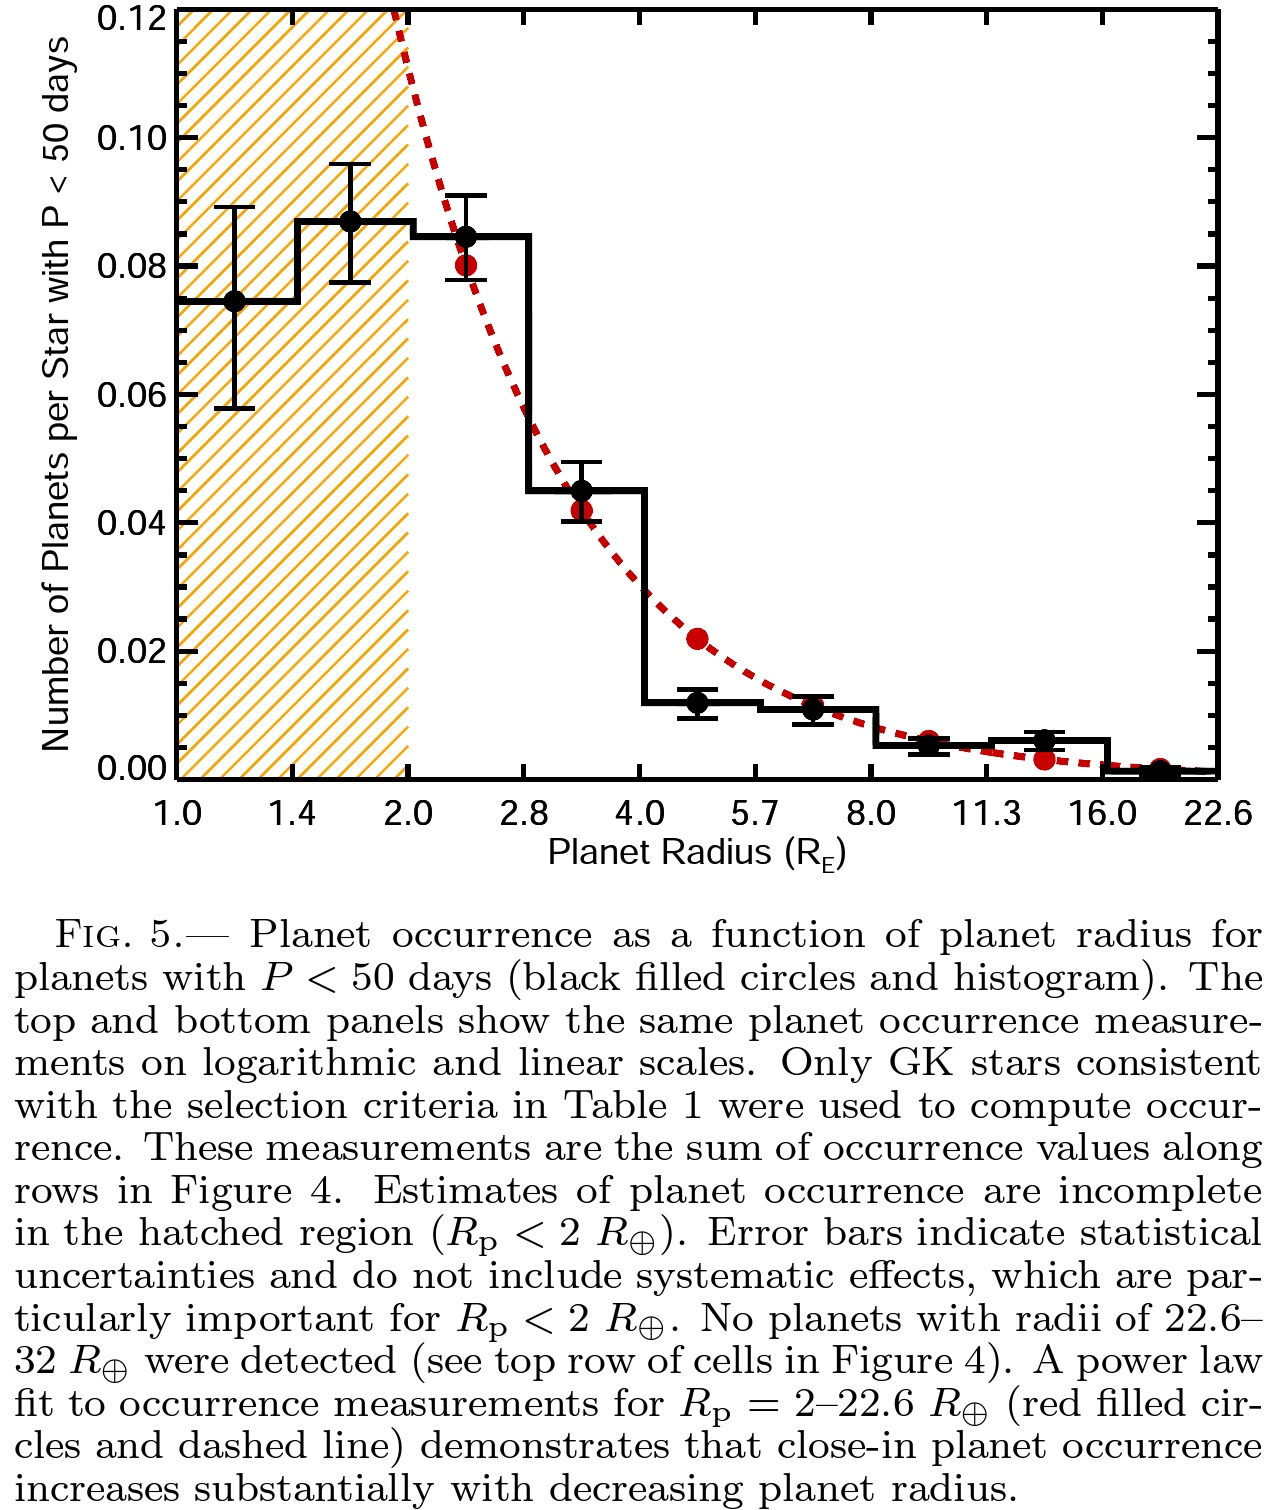
\includegraphics[trim={0cm 22cm 0 0},clip, width=0.95\textwidth,keepaspectratio]{freqvsRpl50d}
		\caption{Distribuzione raggi planetari: crescita esponenziale verso piccoli raggi. La regione barrata indica misure incomplete. Da \cite{howard2012planet}.}\label{fig:howard2012planet}
	\end{subfigure}
	~
	\begin{subfigure}[b]{0.5\textwidth} \centering
		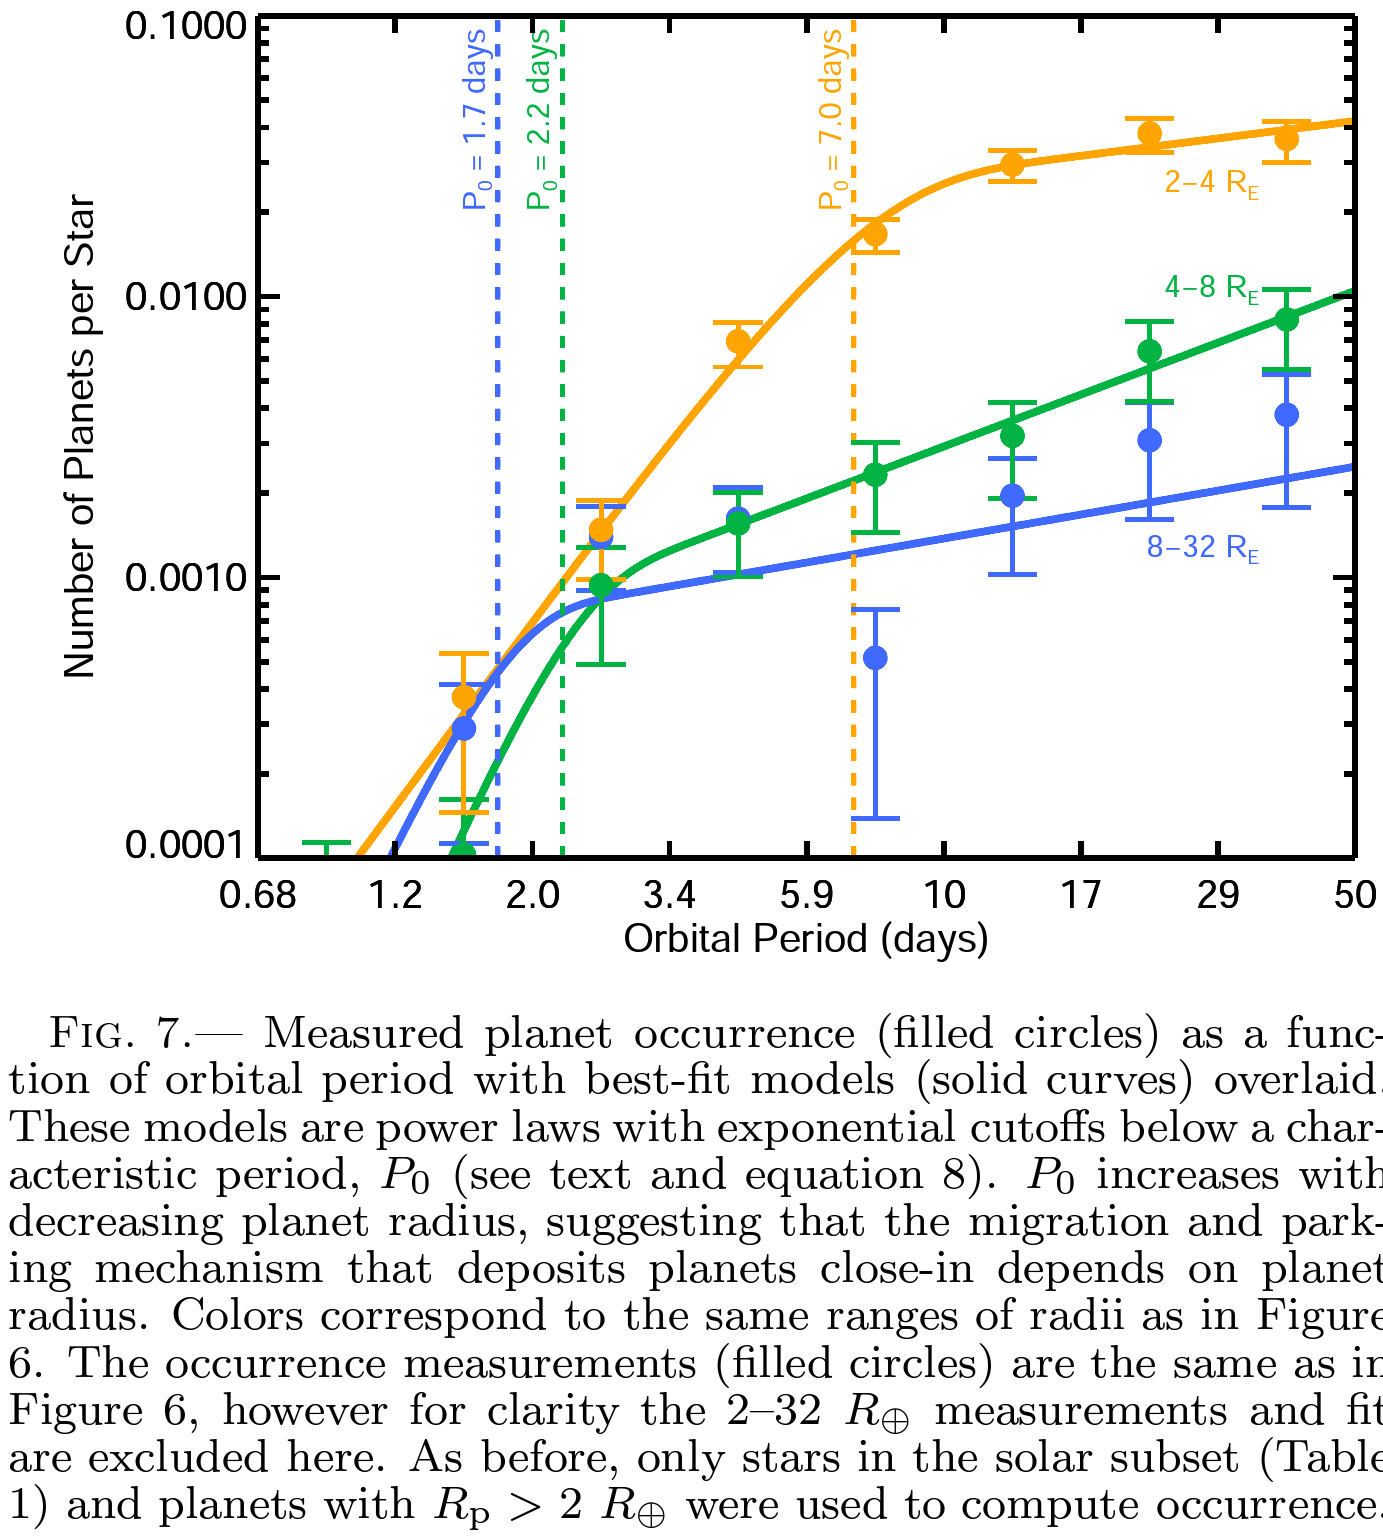
\includegraphics[trim={0cm 19cm 0 0},clip,width=0.95\textwidth,keepaspectratio]{freqperstarvsPanfit}
		\caption{Distribuzione dei periodi orbitali raggruppate per diversi raggi planetari: indicato il diverso periodo critico a cui si ha drastica diminuzione nella distribuzione planetaria. Da \cite{howard2012planet}.}\label{fig:freqperstarvsPanfit}
	\end{subfigure}
\end{figure}

\begin{workout}[Probabilit\'a rivelazione pianeti con orbite eccentriche e durata transito]
	La maggiore probabilit\'a di transito per orbite eccentriche \'e compensata approssimativamente dalla minore probabilit\'a di rilevamento per la minor durata del transito.
\end{workout}

\begin{workout}[ricopiare risultati howard12]
	?
	tab 4 pg 13
\end{workout}
%\begin{align*}
%&\TDy{\log{R}}{f}=k_RR\expy{\alpha}\\
%&k_R=2.9_{-0.4}^{+0.5},\ \alpha=-1.92\pm0.11
%\end{align*}

\begin{workout}[Transit duration]
\[T=(\frac{R_*P}{\pi a}\sqrt{1-b^2})\frac{\sqrt{1-e^2}}{1+e\sin{\omega}}\]
\end{workout}

\begin{workout}[Transity/Doppler discrepancy]
Howard12 pg 20
\end{workout}

\begin{workout}[transit distro observed refs]
Refs:Mthods of detecting exoplanets (radius distro: pg 136)
the occurrence within 0.25 au of solar-type stars from kepler
occurrence architecture exoplanetary
fressin 13: 
petigure 13: plateau PLANET POPULATION BELOW TWICE EARTH SIZE
bathala 13
exoplanet.eu
\end{workout}

\begin{workout}[radius distro]
Local maximum at $1\mjupiter{}$, flat distro in log(r) between $4-10\mearth{}$ below strong increase, at $1.7\mearth{}$ local minimum separating super-earth from sub-neptune
\end{workout}

\begin{workout}[planet model: relazione massa-raggio]
characterization of exoplanets from formation: MR relation pg 18
formazione: vedi \ref{ch:gasaccretion}
MR diagram chabrier 09 (perryman 143)
\end{workout}

\begin{workout}[KEPLER MULTI-PLANET SYSTEM]
THE CALIFORNIA-KEPLER SURVEY. V. PEAS IN A POD: PLANETS IN A KEPLER MULTI-PLANET SYSTEM ARE SIMILAR IN SIZE AND REGULARLY SPACED
III - A gap in radius distribution of small planets
\end{workout}

\begin{workout}[transiti refs: osservabilie probabilit\'a di rilevamento]
pg103
pg 117, eccentric orbit pg 121-122
From space: presence of structure on stellar surface Perryman 3.4, Eriksson Lindegren 07; simulation of stellar jitter: Svensson Ludwig 05, Ludwig 06.
Probability of randomlyoriented planet on circular/eccentric orbit (Borucki Summers 84/Barnes 07, Burke 08,  Seagroves 03, Kane von Braun 08):
\end{workout}

\begin{workout}[Transiti: Propriet\'a dei pianeti a transito]
pg 143, fig 6.33, 6.34, 6.35
Mass-radius relation: chabrier 09
\end{workout}

\begin{workout}[M-R diagram]
orbital migration 10.8 Perryman, tidal effect 10.9, 
fig11.2, 11,4 (EOS), 11.7, 11.8 (M-R)
Ternary diagram 11.9, M-R realtion
Fig 6.33/34/35: mass radius realtion

pg 144: theoretical model - La posizione di un pianeta nel diagramma M-R fornisce indicazione della composizione
fig 6.35
\end{workout}

\begin{workout}[Struttura orbitale e risonanze moto medio]
\end{workout}

\begin{workout}[Long term dynamical stability: mmr, fully packing, eccentricity, inclination distro]
tidal circularization
resonance capture and migration (pg 41)
barnes 08: secularly/resonant dominated
Planets near mmr (Petrovich 12): strength of resonance
P-P scattering leds to tightly packed planetary systems (Raymond barnes 09)
Architecture of planetary systems based om kepler data: number of planets and coplanarity (Fang Margot 12): e,i distro.
Spacing Kepler planets (Wu Pu 15)
Are planetary systems filled to capacity? (Fang Nargot 13)
\end{workout}

\begin{workout}[bimodal radius distro is observed by transit?]
	Characterization of exoplanets from their formation II. The planetary mass-radius relationship pg 21: bimodal radius distribution
\end{workout}

\begin{workout}[Occurence rate]
	\begin{itemize}
	\item Coralie hot jupiter: giant planets $M\sin{i}>0.2\mjupiter$ and $a<0.1au$; $5.6\%$ giant out to 4au
	\item Lick/Keck/AAT ($M\sin{i}>0.5\mjupiter$): $1.2\%$ stars have hot jupiter and $6.6\%$ giant within 5 au
	\item ...
\end{itemize}
\end{workout}

\section{Struttura planetaria: massa, composizione, effetto della radiazione stellare}

\begin{wrapfigure}[18]{l}{0.61\textwidth}
	\centering 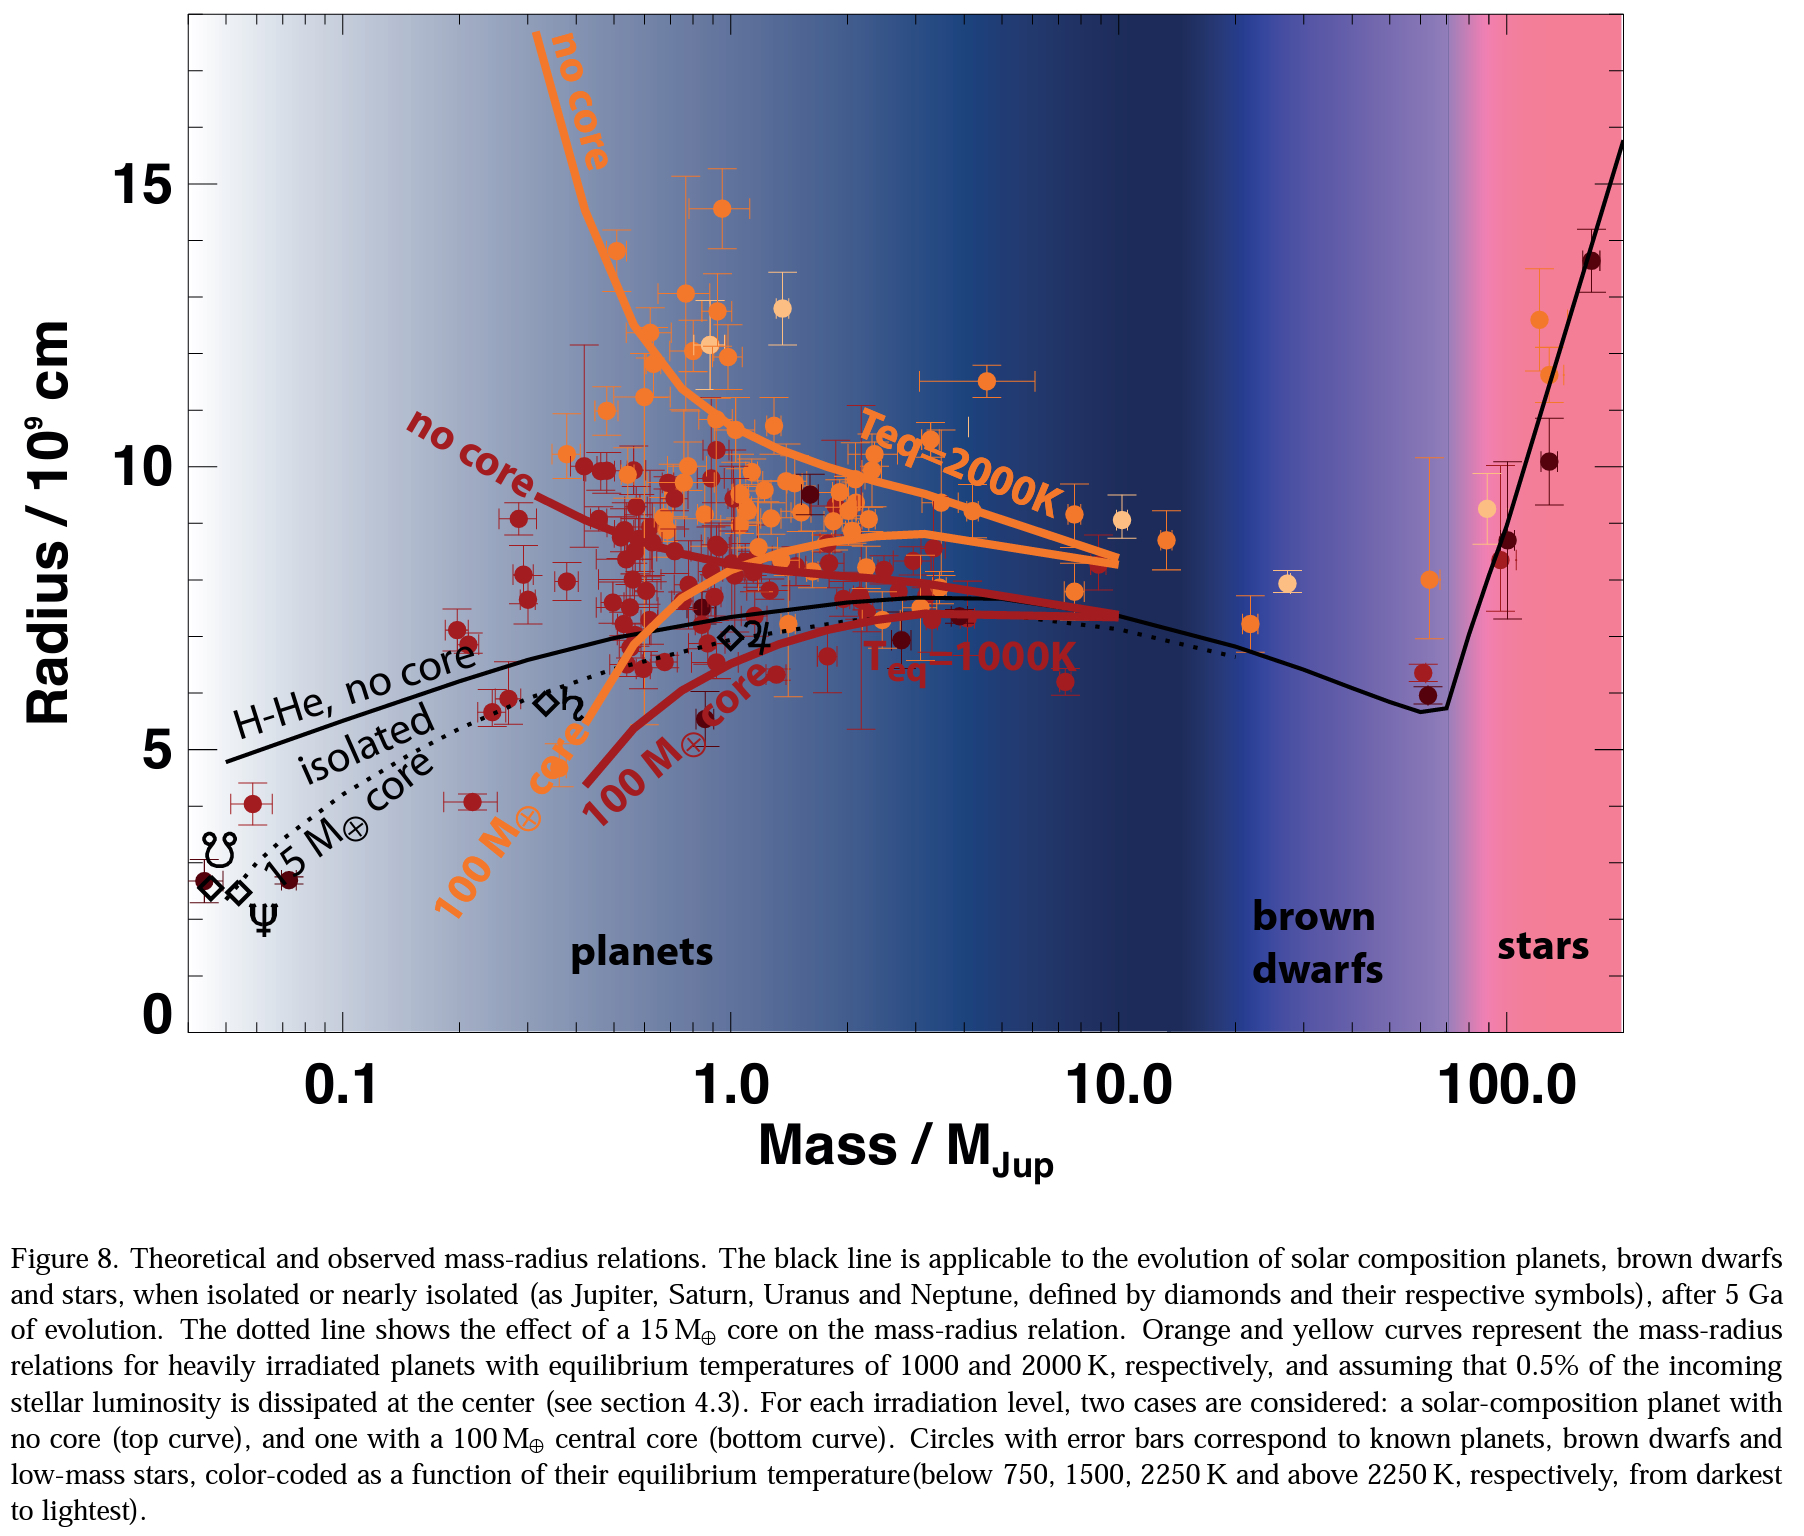
\includegraphics[trim={0cm 12cm 0 0},clip, width=0.6\textwidth]{MR-model-obs}
	\caption{Relazione massa-raggio determinata sulla base di modello planetario dopo \SI{5}{\giga\year}. Per gli esopianeti sono indicate le curve per temperature di equilibrio di \SI{1000}{\kelvin} e \SI{2000}{\kelvin}. Da \cite{guillot2014giant}.}\label{fig:MR-model-obs}
\end{wrapfigure}

Dati raggio e massa di un pianeta \'e possibile determinare la struttura interna e la composizione tramite un modello planetario. 

%la posizione di un pianeta nel diagramma massa-raggio \'e determinata dalla storia di accrescimento del pianeta (composizione), dal'organizzazione interna del materiale e dall'irraggiamento stellare.
%e propriet\'a di H/He e metalli a alte densit\'a (rottura H molecolare, ionizzazione da pressione, degenerazione elettronica, transizioni di fase).
\begin{workout}[Earth-super Earth, Neptune-Super Jupiter]
Baraffe pg 18
\end{workout}
\begin{workout}[Evaporazione]

\end{workout}
\begin{workout}[EOS]
	Stiffness: bulk modulus $K_{S/T}=\rho(PDy{\rho}{P})_{S/T}$
	Solid: finite density as P goes to 0 - $\rho\approx\rho_0(1+P/K)$ - $R\propto M\expy{1/3}$
H:
\end{workout}
\begin{workout}[popolazioni: earts-super, neptunian, sub-giant, giant, habitable]

\end{workout}

La figura (\ref{fig:MR-model-obs}) mostra la relazione massa-raggio per pianeti nettuniani fino a regimi stellari: si ha un diverso comportamento nel diagramma M-R per pianeti con diversa struttura interna o per alte temperature di equilibrio dovute alla radiazione stellare p(opolazione dei giganti gassosi).
%Effetti della radiazione stellare: evaporazione, differente temperatura di equilibrio del pianeta
%Le fonti di incertezza dei modelli planetari sono l'equazionbe di stato e la distribuzioni della componente metallica.
Per quanto rigurda l'equazione di stato per idrogeno ed elio ad alte pressioni si ha completa ionizzazione degli elementi e la pressione \'e fornita dalla degenerazione degli elettroni: per una relazione politropica
\begin{equation}
P\propto\rho\expy{\gamma},\ \gamma=\frac{1}{n}+1
\end{equation}
la relazione massa raggio \'e
\begin{equation}
R\propto M\expy{(1-n)/(3-n)}
\end{equation}
Per $M\approx\mjupiter$ $n\approx1$ quindi il raggio \'e approssimativamente costante: questo fatto \'e visibile anche nella distribuzione dei raggi planetari (figura \subref{fig:probvsR-T}) nel picco attorno a $\rjupiter$. La figura (\subref{fig:hydrogeneosJSUN}) sovrappone al diagramma $P-T$ dell'idrogeno il profilo nel diagramma di alcuni pianeti gassosi.
\begin{figure}[!ht]
	\begin{subfigure}[t]{0.49\textwidth}
		\centering
		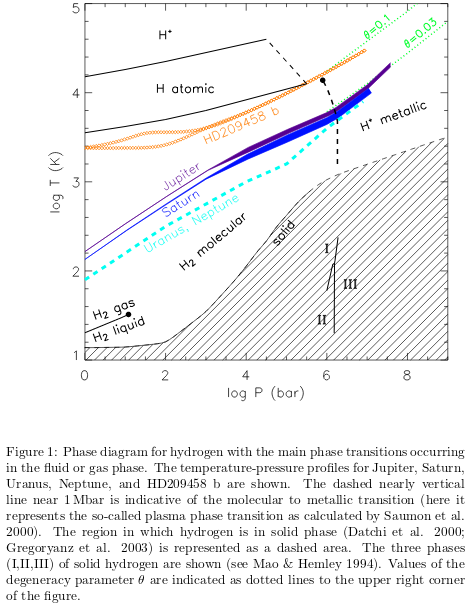
\includegraphics[trim={1.7cm 7.3cm 0.7cm 0},clip, width=0.95\textwidth,keepaspectratio]{hydrogeneosJSUN}
		\caption{Diagramma di fase dell'idrogeno. Le regioni in cui si ha $H_2$ molecolare e $H^+$ metallico sono separate da line tratteggiata nera. La regione in cui si ha solidificazione \'e tratteggiata con indicazione delle 3 diverse fasi (I,II,III). Valori del parametro di degenerazione $\theta=\frac{T}{T_F}$. Profilo nel piano $T-P$ dei pianeti HD209458 b, Giove, Saturno, Urano e Nettuno. Da \cite{guillot2005interiors}.}\label{fig:hydrogeneosJSUN}
	\end{subfigure}
	~
	\begin{subfigure}[b]{0.49\textwidth} \centering
		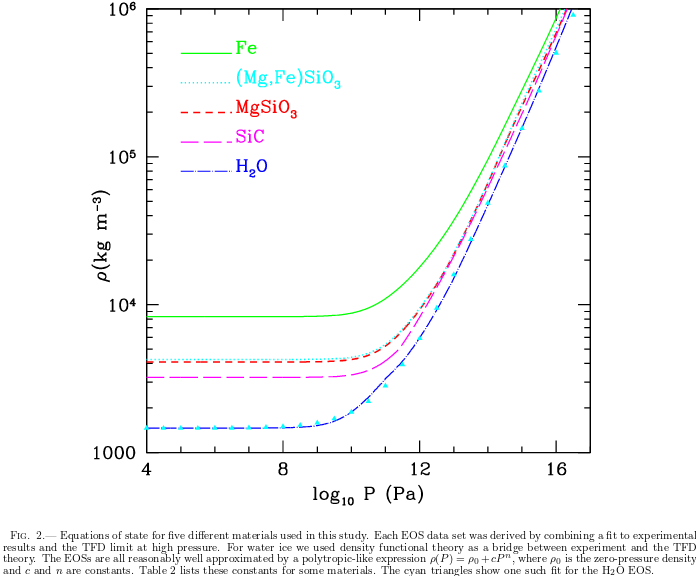
\includegraphics[trim={3cm 2.5cm 3.5cm 0},clip,width=0.95\textwidth,keepaspectratio]{solideos}
		\caption{Equazione di stato per alcuni elementi della componente solida. Da \cite{howard2012planet}.}\label{fig:solideos}
	\end{subfigure}
\end{figure}

L'equazione di stato della componente pi\'u pesante di idrogeno ed elio \'e approssimabile da:
\begin{equation}
\rho(P)=\rho_0+cP^n
\end{equation}

Oltre ad aumentare la temperatura di equilibrio nei pianeti vicini la radiazione solare causa perdita di massa dagli strati superiori dell'atmosfera. Il flusso $F_{XUV}$ di fotoni a \SIrange{1}{1200}{\angstrom} (\cite{ribas2005evolution}) riscalda gli strati esterni dell'atmosfera e si genera un flusso uscente di componente volatile (\cite{lopez2013role}):
\begin{align}
&\dot{m}=\epsilon\frac{\pi F_{XUV}R_{XUV}^3}{GM_pK_{tide}}\\
&K_{tide}=1-\frac{3}{2\xi}+\frac{1}{2\xi^2},\quad\xi=\frac{R_H}{R_{XUV}}
\end{align}
dove il raggio a cui l'atmosfera \'e opaca per XUV \'e $R_{XUV}$, $K_{tide}$ tiene conto del fatto che \'e sufficiente che le particelle giungano a una distanza pari al raggio di Hill.
La figura (\subref{fig:RfreqPl100ub}) mostra due picchi nella distribuzione radiale a $1.3\rearth{}$ e $2.4\rearth{}$ dovuti alle sottopopolazioni di pianeti rocciosi e gassosi per $P<\SI{100}{\day}$: i pianeti rocciosi hanno atmosfera di H/He che non contribuisce alle dimensione mentre i pianeti nettuniani hanno strato di gas consistente rispetto alla massa del pianeta. La valle a $1.7\rearth{}$ potrebbe essere il raggio di separazione tra pianeti terrestri con atmosfera tenue di H/He soggetta a evaporazione e pianeti nettuniani con massa consistente di H/He.

\begin{figure}[!ht]
\begin{subfigure}[b]{0.49\textwidth}
	\centering 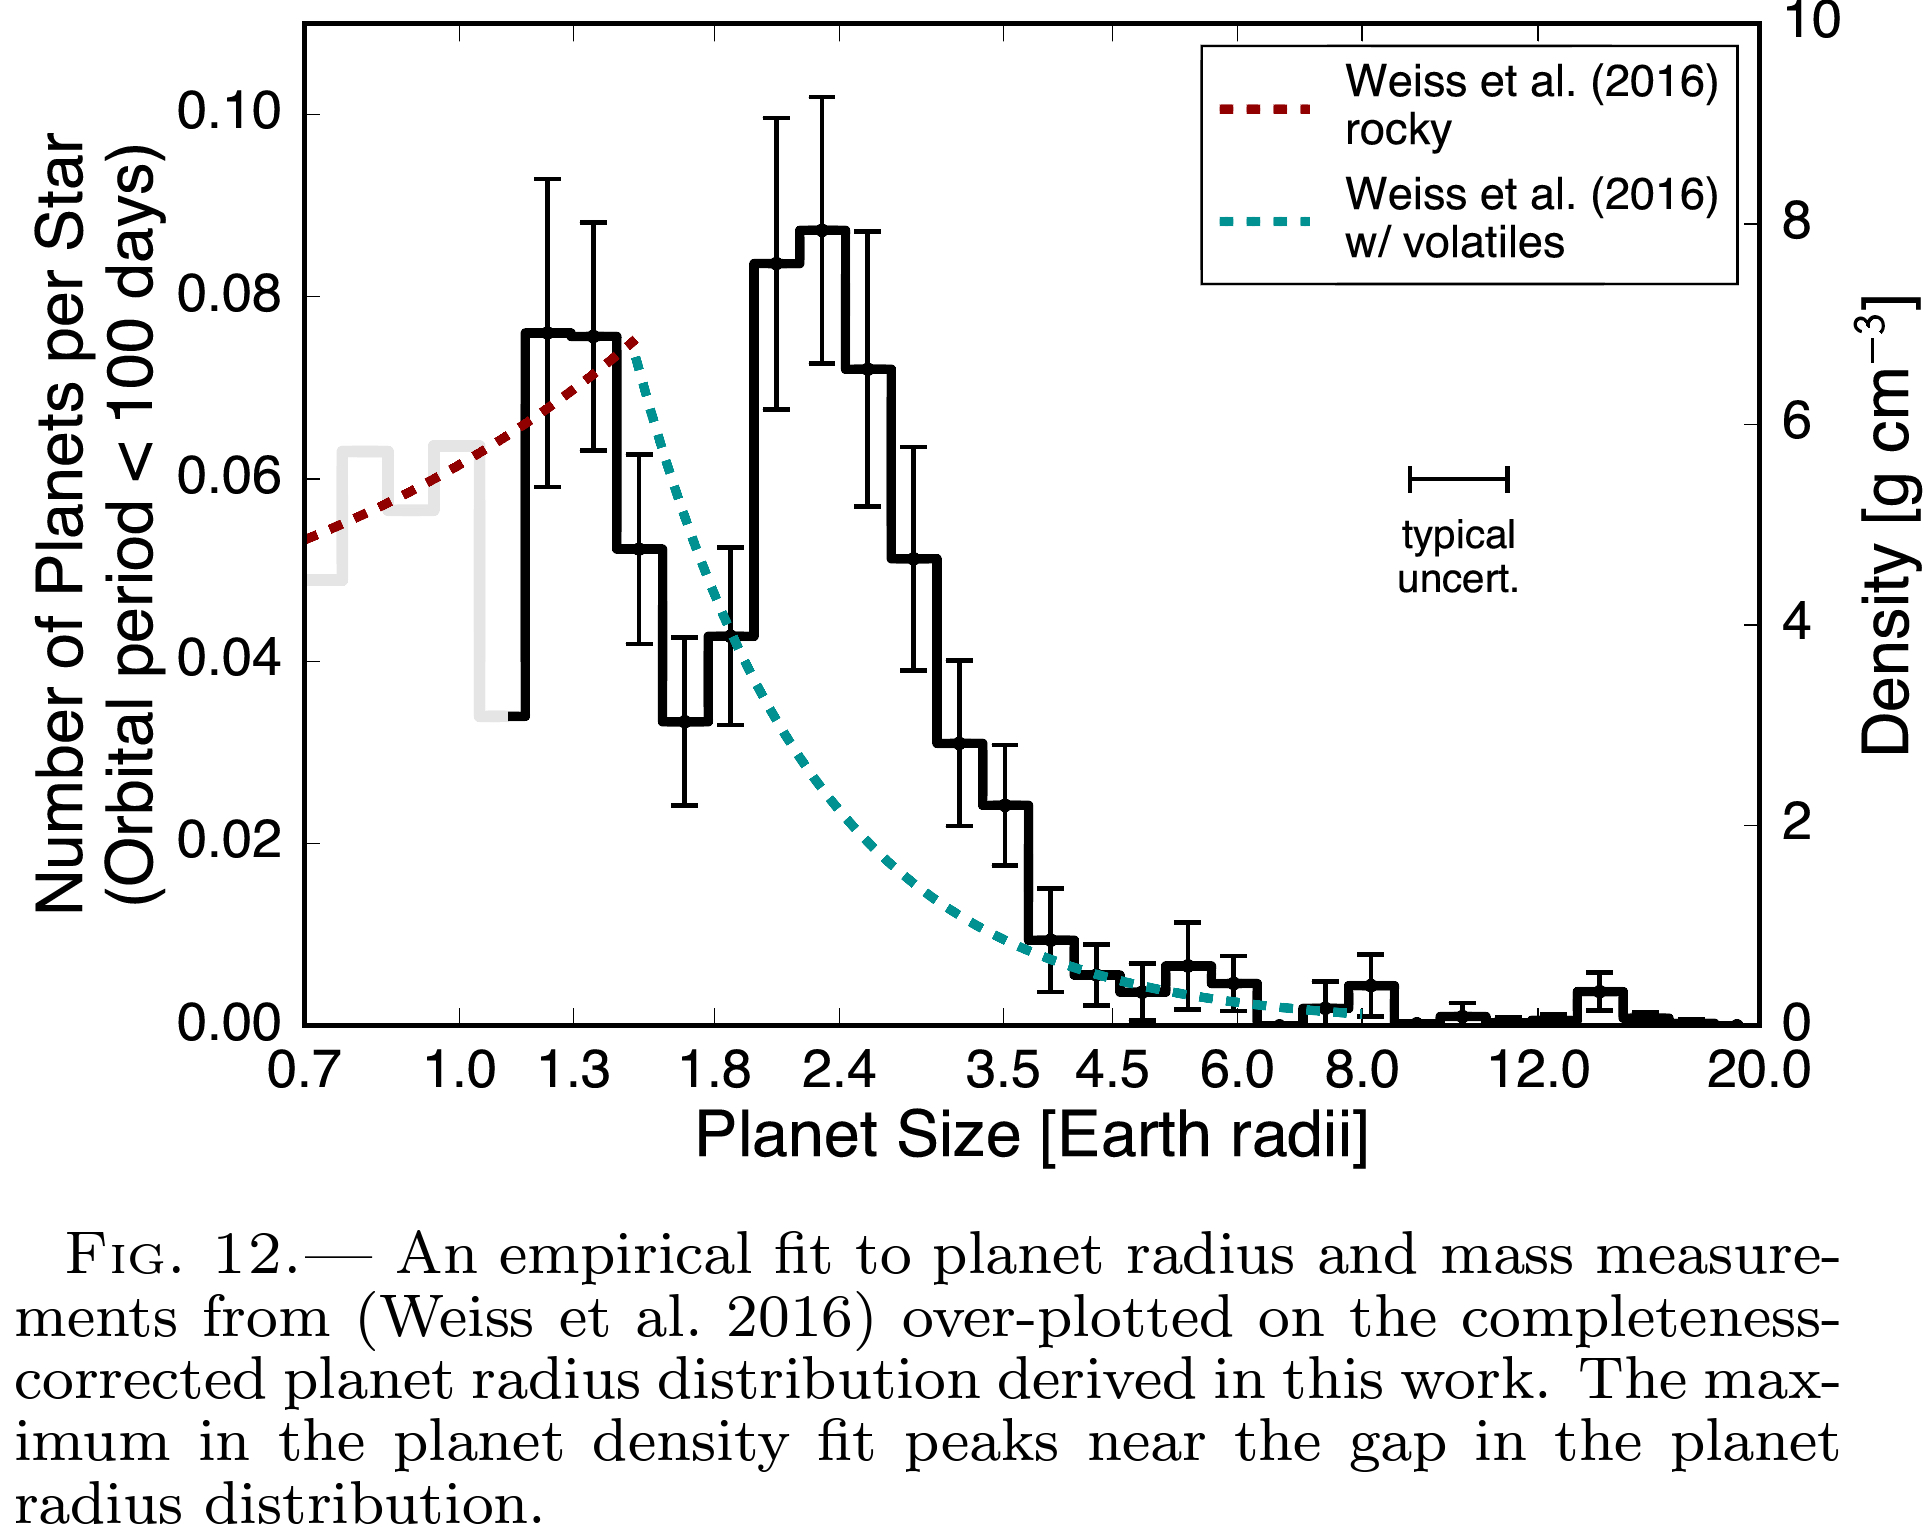
\includegraphics[trim={0 12cm 0 0},clip, width=0.95\textwidth]{RfreqPl100ub} 
	\caption{Distribuzione per i pianeti osservati tramite transito con $P<\SI{100}{\day}$: la valle a $1.7\mearth{}$ si ipotizza causato dall'evaporazione. Da \cite{fulton2017california}.}\label{fig:RfreqPl100ub}
\end{subfigure}
~
\begin{subfigure}[b]{0.49\textwidth}
	\centering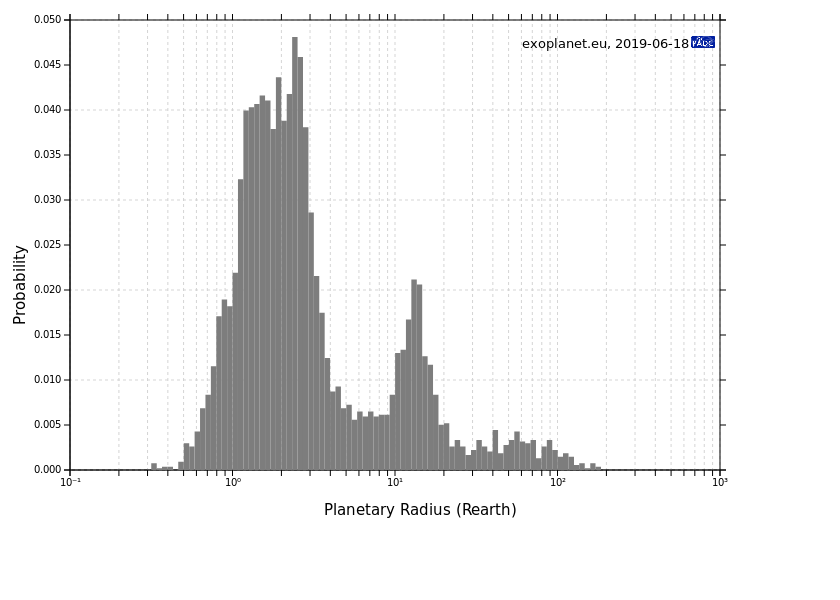
\includegraphics[trim={0cm 0.5cm 0 0},clip, keepaspectratio,width=0.99\textwidth]{Rfreq}\caption{Distribuzione radiale pianeti rivelati tramite T. Da \cite{exoplanet.eu} (luglio 2018): la frequenza ha andamento crescente verso pianeti di raggio terrestre, andamento piatto tra $4-10\rearth{}$ e picco a $R\approx\rjupiter{}$.}\label{fig:probvsR-T}
\end{subfigure}
\end{figure}

\begin{workout}[Mass-Metallicity relation for giant planet: ''Mass-metallicity relation for giant planets'' (Thorngren 16)]
	Solve equation for planetary structure to infer $M_c+M_e$ assuming $M_c\approx10\mearth{}$; search correlations between $M_p$, $M_z$ and $[Fe/H]$, $Z_p$ and $Z_p/Z*$.
	Negative correlation between planet's metal enrichment relative to its parent star: MF11, mordasini 14.
	\begin{align*}
	&M_p=M_c+M_e,\ M_Z=M_c+Z_*M_eZ_p=M_z/M_p\\
	&Z_p/Z_*=1+(M_c/M_p)(1-Z*_)/Z_*
	\end{align*}
	latter expression fall off more rapidly with planet mass  than $Z_p/Z_*\approx10(M_p/M_J)\expy{-0.5}$ (later accretion of planetesimal debris Mousis 09)
\end{workout}

\begin{errata}[Equazione di stato politropa: relazione massa raggio]
	\begin{equation}
	P\propto\rho\expy{\gamma},\ \gamma=\frac{1}{n}+1
	\end{equation}
	si che per $M\approx\mjupiter$ $n\approx1$.
	Inoltre la relazione massa-raggio  \'e approssimabile
	\begin{equation}
	R\propto M\expy{(1-n)/(3-n)}
	\end{equation}
\end{errata}

%\begin{figure}[!ht] \centering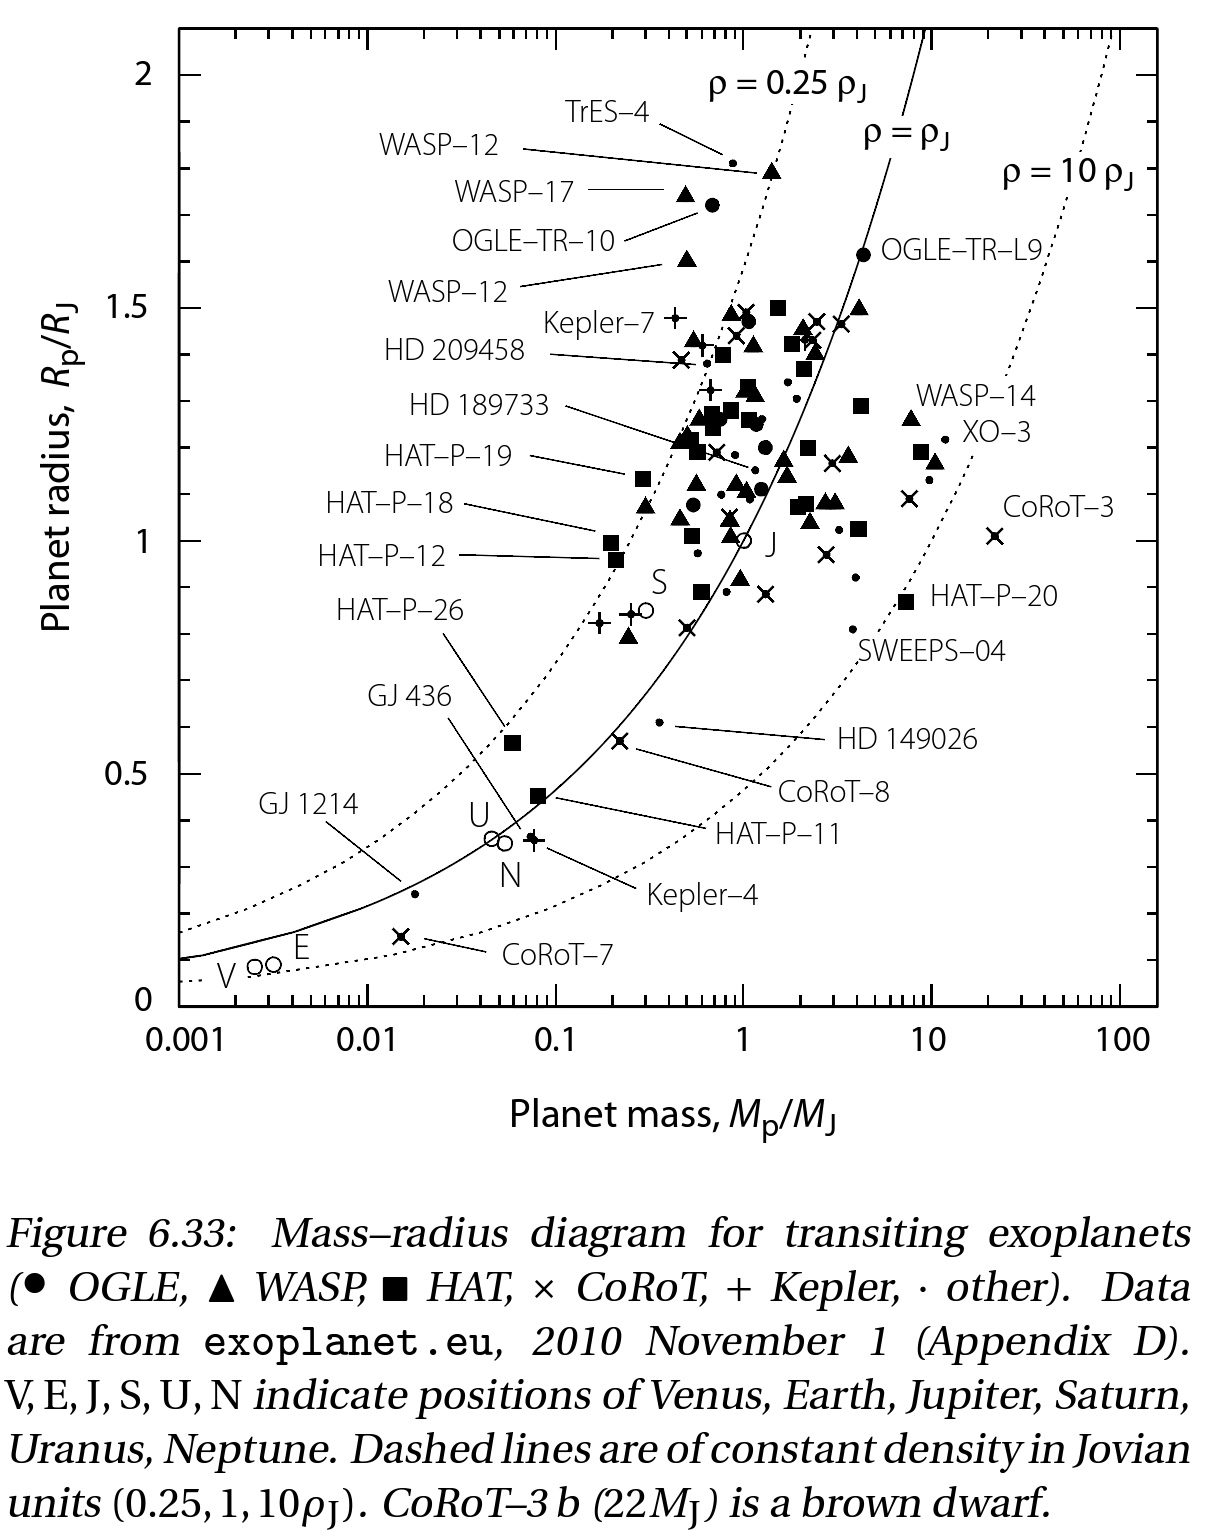
\includegraphics[trim={0cm 14cm 0 0},clip, keepaspectratio,width=0.9\textwidth]{MRD}\caption{Diagramma mass-raggio per pianeti di transito. Le curve tratteggiate sono a densit\'a costante. Il simbolo $\circ$ indica i pianeti del sistema solare. Da \cite{perryman2011exoplanet}.}\label{fig:MRD}
%\end{figure}

%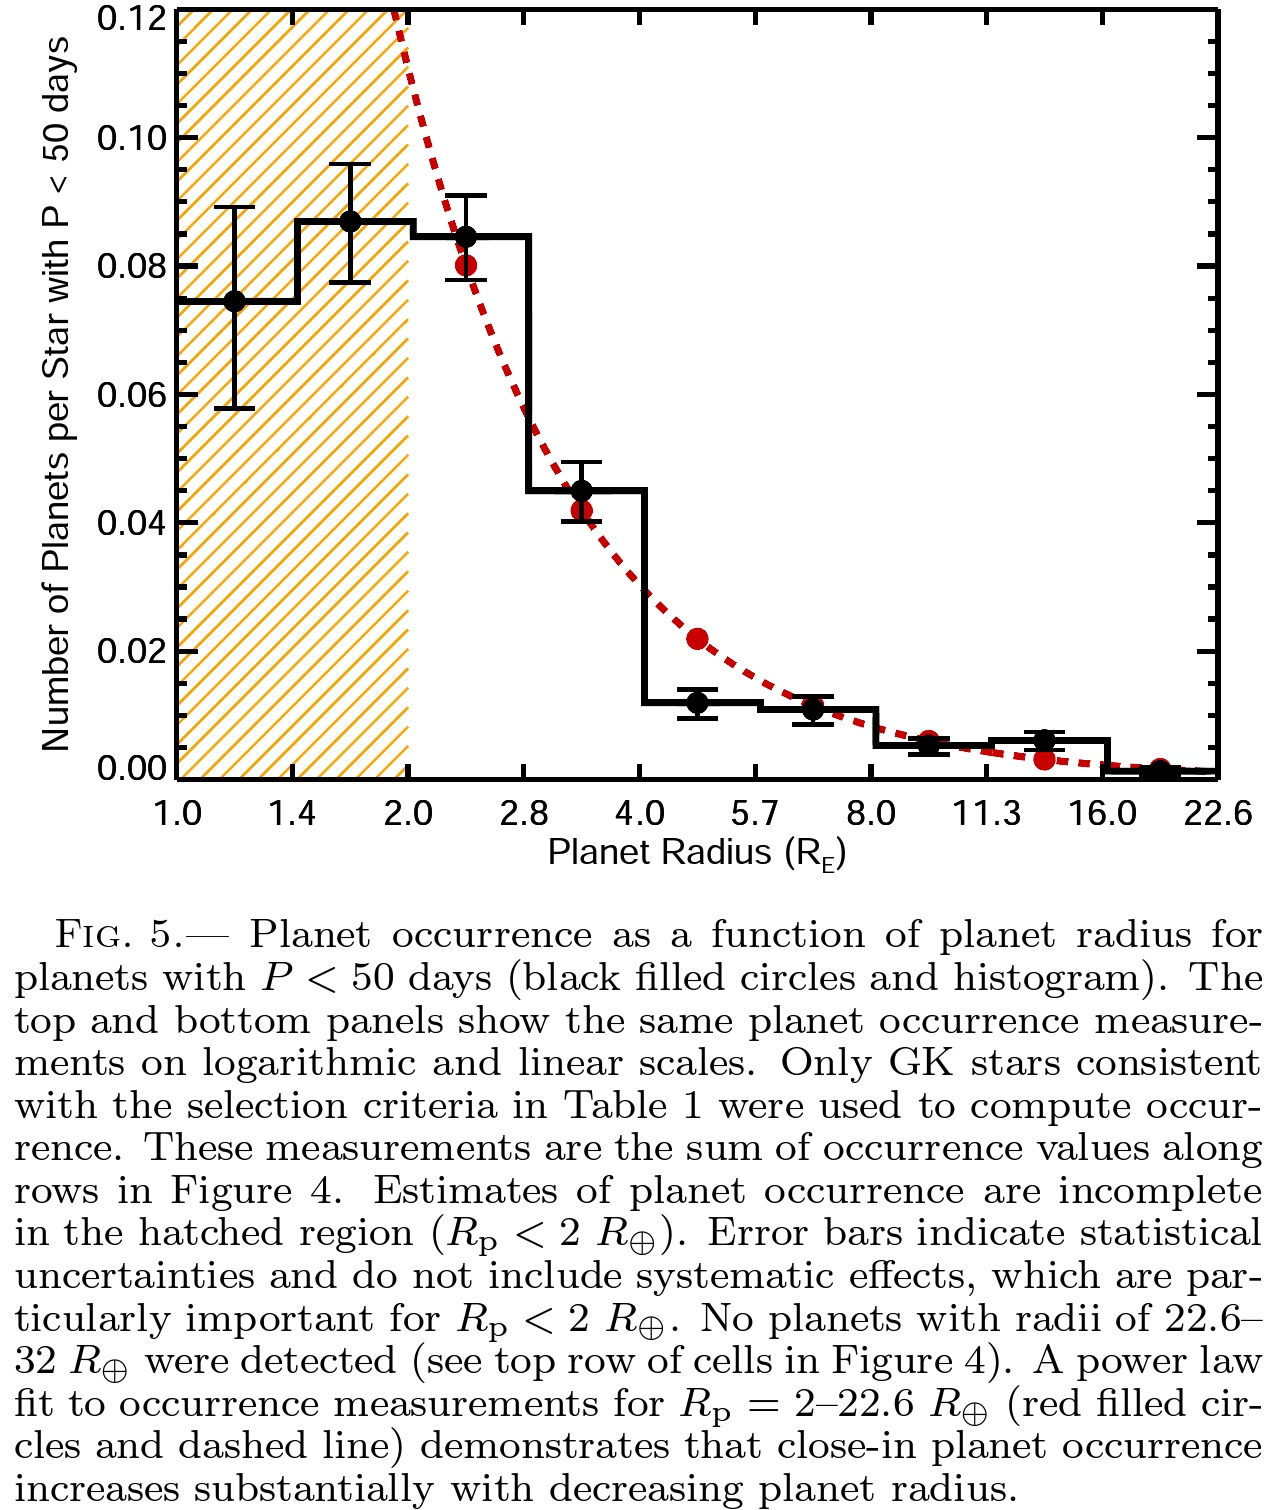
\includegraphics[trim={0cm 0 0 0},clip, keepaspectratio,width=0.9\textwidth]{freqvsRpl50d}\label{freqvsRpl50d}\caption{Da \cite{howard2012planet}}
% 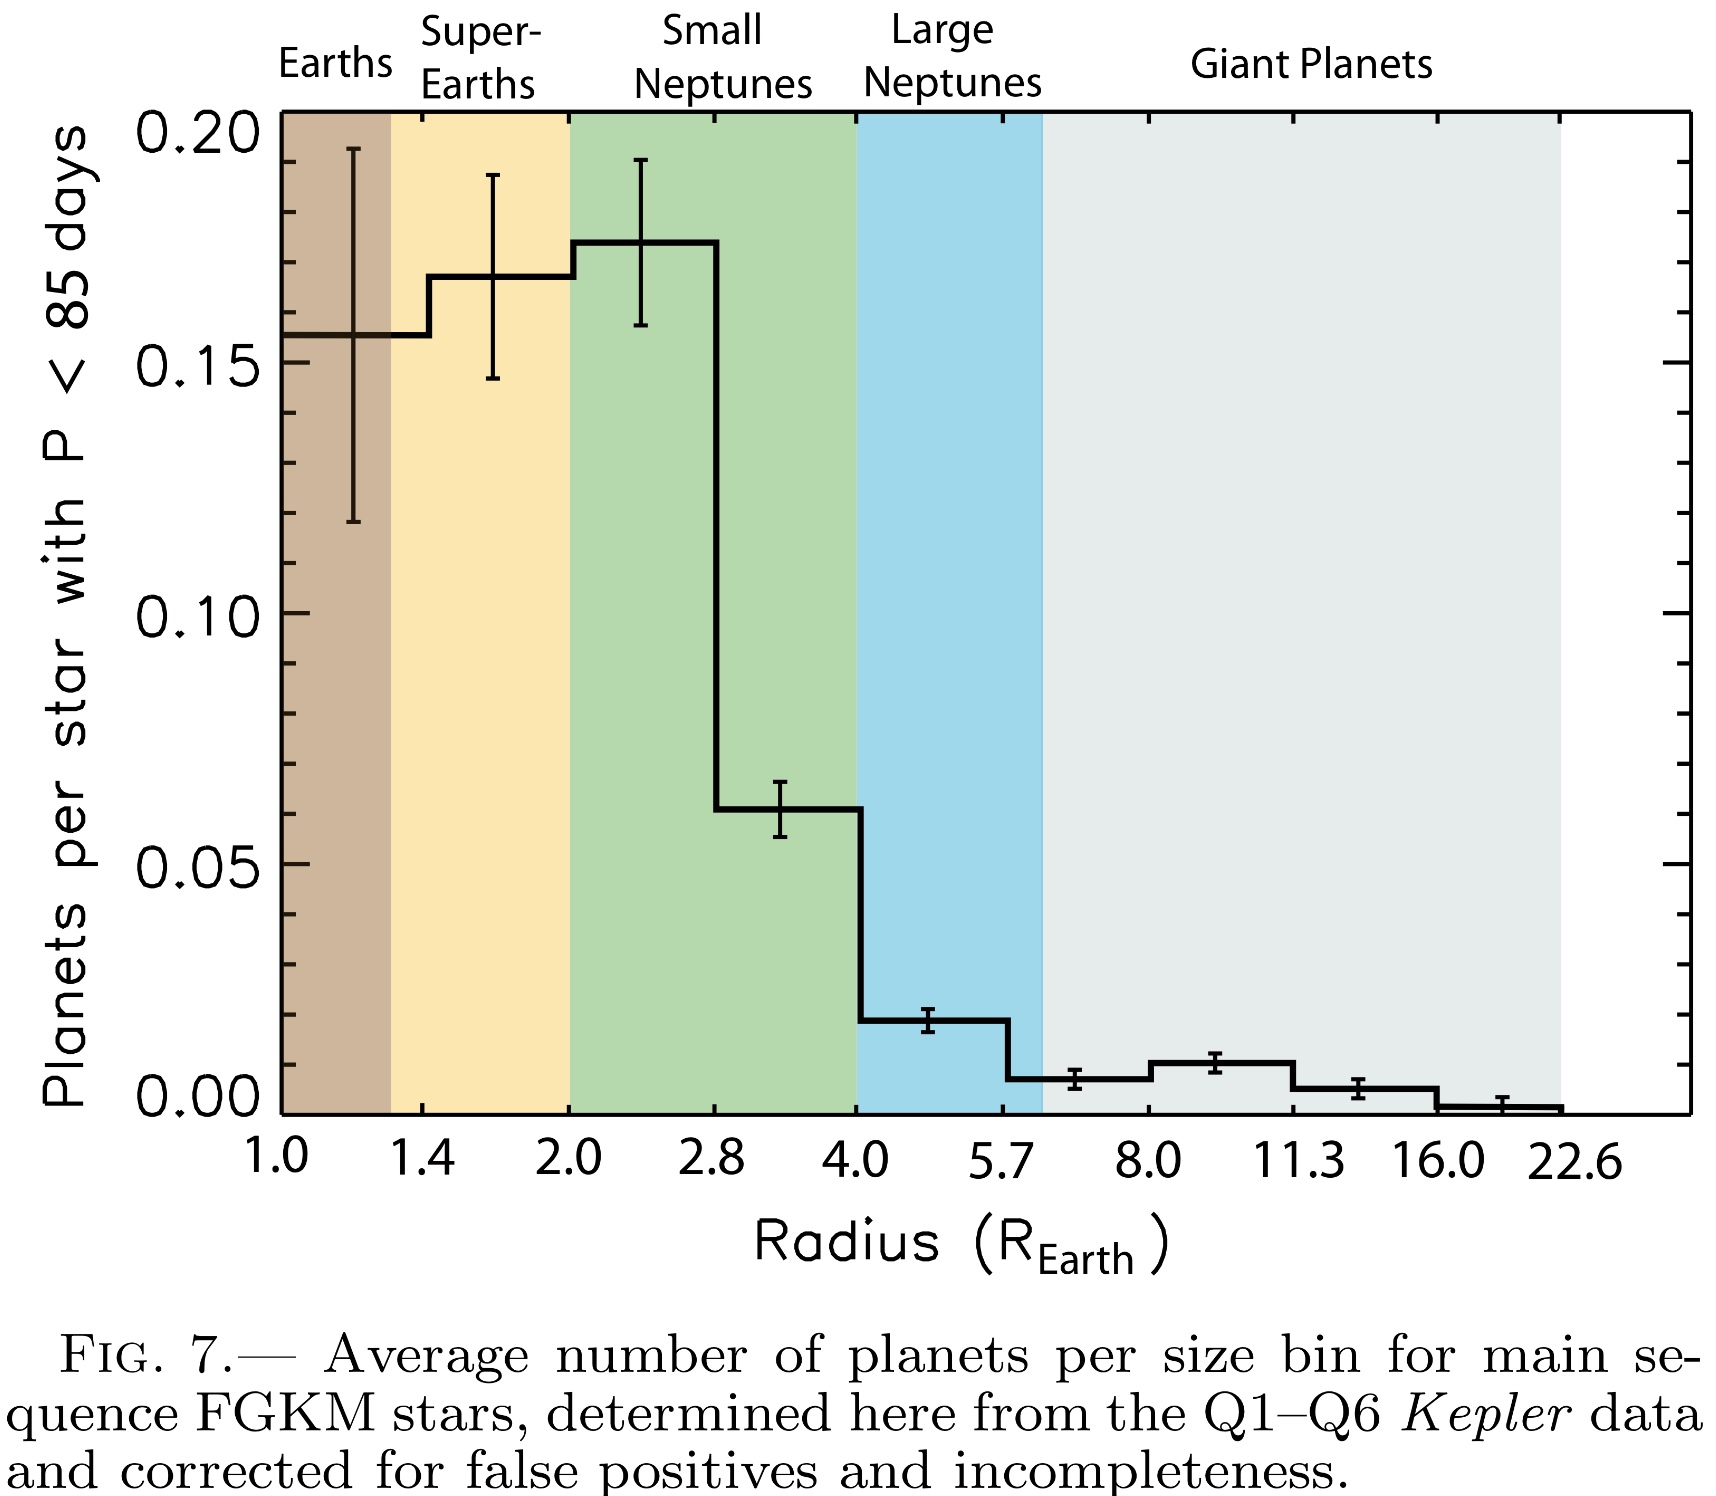
\includegraphics[trim={0cm 0 0 0},clip,width=0.95\textwidth]{keplerRfreq}\label{fig:keplerRfreq} \caption{Da \cite{fressin2013false}}
%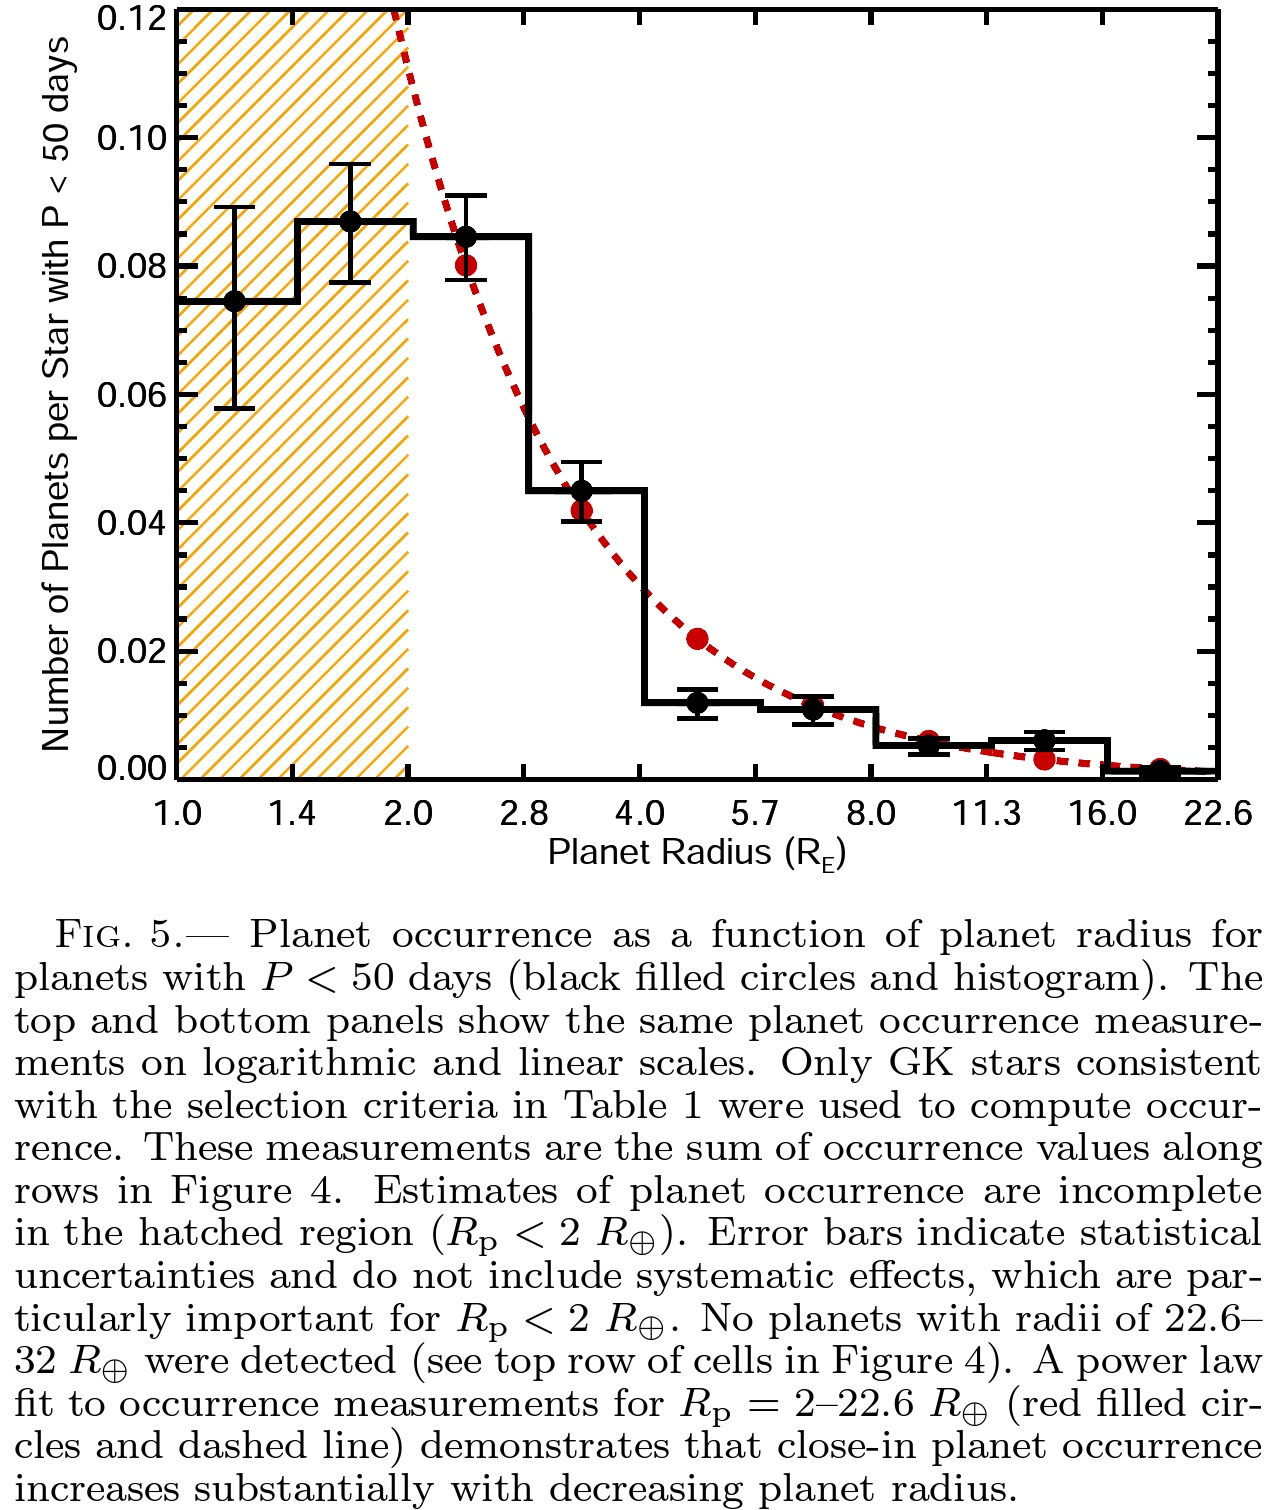
\includegraphics[trim={0cm 0 0 0},clip, keepaspectratio,width=0.9\textwidth]{freqvsRpl50d}\label{fig:freqvsRpl50d}\caption{Da \cite{}.}

\begin{workout}[sottosezione propriet\'a orbitali]

\end{workout}




\begin{workout}[Some refs]
	\begin{itemize}
		\item Lamb 32: amount of energy converted in turbulent motion
	\end{itemize}
\end{workout}

%Jansky=10-23erg/(s*cm2*Hz)
\begin{workout}[Refs dischi protoplanetari]
	Chronology of  early stages: apai lauretta 10 (book)
\end{workout}

\begin{workout}[Condizioni iniziali: formazione planetesimi, caratteristiche dischi protoplanetari]
	Chronology of  early stages: apai lauretta 10 (book)
\end{workout}

\begin{workout}[Profilo densit\'a verticale disco isotermo]
	Thin vertically isothermal disk
	\begin{align}
		&\rho(z)=\frac{\Sigma}{h\sqrt{2\pi}}\exp{-\frac{z^2}{2h^2}}\\
		&
	\end{align}
\end{workout}

\begin{workout}[Profilo termico del disco]
	
\end{workout}

\begin{workout}[Momento torcente in disco Kepleriano]
	\begin{align}
		&\sigma_{ij}=2\Sigma\nu D_{ij}=\Sigma\nu\begin{pmatrix}0&-\Omega\partial_r(r\Omega)\\-\Omega+\partial_r(r\Omega)&0
		\end{pmatrix}\\
	\end{align}
	Il momento torcente esercitato da S su $C^c$ \'e
	\begin{equation}
	T=\iint_{S^c}(\vec{r}\wedge\nabla\sigma)\,ds=\int_S\vec{r}\wedge(\sigma\,dl\vec{n})
	\end{equation}
	Nel caso S sia circonferenza di raggio r:
	\begin{equation}
	T_{\nu}=3\pi r^2\Omega_0\Sigma\nu
	\end{equation}
\end{workout}

\begin{workout}[Struttura verticale del disco, profilo termico]
	Pressione gas determinata da equilibrio idrostatico
	Passive disk (Refs: Ref: spectral energy distribution of T-Tauri star with passive circumstellar disk)	Dust passively reirradiate star light
\end{workout}

\begin{workout}[Viscous/turbulent disk]
	laminar (high momentum diffusion)
	mass inflow Gullbring98 \SIrange{e-9}{e-7}{\per\year}$\msun{}$
\end{workout}
\begin{workout}[MRI]
	fig 10.3:
	gammie 1996
\end{workout}

\begin{workout}[alpha prescription]
	$\vec{v}=(u_r,r\Omega)$, stress tensor $\sigma_{r\phi}=-\Sigma\exv{u_ru_{\phi}}$.
	Enhanced turbulent viscosity: $-\Sigma\exv{u_ru_{\phi}}=\Sigma\nu r\TDy{r}{\Omega}$, $\nu=v_TH$, $\alpha=v_T/c_s$
\end{workout}

\begin{workout}[Accretion disk sources]
	Lodato: classical disk physics
	o218, 296: disk formation, constrains from solar system
	the alpha disk pg 18: theory of turbulent accretion disk
\end{workout}


\begin{workout}[Descrizione trasporto momento angolare tramite parametrizzazione viscosit\'a]
	Mass conservation + momentum conservation in viscous flow: angular momentum evolution. Phenomena: Shear viscosity - turbulence - MRI.
	Nei modelli 1D per disco di accrescimento si parametrizza viscosit\'a tramite $\nu=\frac{\eta}{\rho}\to\alpha c_s H$: la viscosit\'a molecolare \'e troppo bassa  per trasportare all'esterno il momento angolare sui tempi-scala osservati.
	Theory of turbulent accretion disk: pg 18, 8.
	Flusso di x-momentum lungo y $\rho\exv{u_xu_y}$, dove considero la velocit\'a dell'elemento di fluido $(v_x+u_x,u_y)$ dove le $u$ rappresentano fluttuazioni della velocit\'a: $\sigma_{xy}=-\rho\exv{u_xu_y}$.
	Ricordando la definizione di tensore degli stress e con $\vec{v}=v_x(y)\hat{x}$
	\begin{equation}
	\sigma_{ij}=\eta(\partial_jv_i+\partial_iv_j-\frac{2}{3}\delta_{ij}\partial_kv_k+\zeta\delta_{ij}\partial_kv_k \to \eta\TDy{y}{v_x}
	\end{equation}
	\begin{equation}
	\PDof{t}(\rho v_i)+\PDof{x_i}(\rho v_iv_j+T_{ij})=F_i
	\end{equation}
	Fluttuazioni: $\sigma_{ij}=-\rho\exv{u_iu_j}$.
	Viscosit\'a molecolare: $\exv{u_iu_j}=-\nu\TDy{x_j}{v_i}$.
	Turbulence: Reynpold stress $\tau_{ij}=-\rho\exv{v_jv_i}$, $\exv{u_iu_j}=-\nu_T\TDy{x_j}{v_i}$
	\begin{equation}
	\PDy{t}{\Sigma}=3\frac{1}{r}\PDof{r}[r\expy{1/2}\PDof{r}(\nu\Sigma r\expy{1/2})]
	\end{equation}
\end{workout}

\begin{workout}[Photoievaporation: X-EUV-FUV (Alexander13: The Dispersal of Protoplanetary Disks)]
	Protoplanetary disc evolution and dispersal: the implications of X-ray photoevaporation.
	(Photoevaporation: veras armitage 2003, Alexander13, Mordasini12. Internal/External).
	EUV($E\approx13.6eV$): ionization, FUV($E\approx6-13.6eV$): dissociation, X-ray
\end{workout}

\begin{workout}[classificazione YSO]
	section{YSO: distribuzione propriet\'a dischi protoplanetari}
	La classificazione empirica degli young stellar object (YSO) si basa sul valore di
	\begin{equation}
	\alpha_{IR}=\TDly{\lambda}{\lambda F_{\lambda}}
	\end{equation}
	tra \SIrange{2.2}{25}{\micro\meter}.
	\begin{itemize}
		\item Classe 0: Picco emissione in regione da lontano infrarosso a sub-millimetrica. Nubi molecolari compatte/protostelle.
		\item Classe 1: $\alpha_{IR}>0$ a \SI{2}{\micro\meter}. La stella accresce la maggior parte della sua massa finale.
		\item Classe 2: $0\geq\alpha_{IR}\geq-1.5$. Stella T-Tauri con disco otticamente spesso a $\lambda\leq\SI{10}{\micro\meter}$.
		\item Classe 3: $\alpha_{IR}\leq-1.5$. Stella T-Tauri con disco otticamente sottile a $\lambda\leq\SI{10}{\micro\meter}$.
	\end{itemize}
\end{workout}

\begin{workout}[Fit SED]
	Disk model
	\begin{align}
		\nu\propto R\expy{\gamma}\\
		\Sigma=(2-\gamma)\frac{M_d}{2\pi R_c^2}(\frac{R}{R_c})\expy{-\gamma}\\Exp{-(\frac{R}{R_c})\expy{2-\gamma}}
	\end{align}
\end{workout}


\begin{workout}[Initial conditionfor protostellar collapse]
	Andre 2000 - 
\end{workout}

\begin{workout}[physical processes in protoplanetary disk: IRexcess, accretion rate and lifetime,]
	(armitage 17): fig 1, accretion rate and lifetime (2.2 pg 5-6), inference from dust continuum (disk mass, evidence for mm-particle growth
	Le stelle giovani sono caratterizzate da eccesso infrarosso fra \SIrange{2.5}{10}{\micro\meter}:
	\begin{equation}
	\alpha_{IR}=\TDly{\nu}{\nu F_{\nu}}
	\end{equation}
	Sorgenti con SED declinante in mid infrared ($2.5-10\si{\micro\meter}$): $1.5<\alpha_{IR}=<0$. Active/passive: mass infall convert G into thermalradiation/reprocessed starlight.
	Refs: Perrymann 10.3 - disk formation pg 218 - 
	Classification based on slope of SED between $2-25\si{\micro\meter}$: $\alpha_{IR}=\TDly{\nu}{\nu F_{\nu}}=$ (Gail Hoppo 2010)
	Spitzer: forming regions within 500pc
	Formation: disk quickly forms as more distant material with high angular momentum, centrifugal radius $R(t)\propto\Omega^2 t^3$: . Class 0-I : protostellar disk, gravitational unstable (cloud collapse: the collapse of the cores of slowly rotating isothermal clouds, Terebey shu cassen 1984, selfsimilar collapse of isothermal spheres and star formation, shu 77). Singular isothermal sphere: $\rho=\frac{a^2}{2\pi G}r\expy{-2}$, $M(r)=\frac{2a^2}{G}r$.
\end{workout}

\begin{workout}[disco protoplanetario: distribuzioni condizioni iniziali]
	
	Initial disk mass
	(infall phase end, no more self-gravitational instabilities) - stability(shu90), MMSN hayashi81/weidenshilling77, observations(Andrews10,Manara16) points to $(0.1-10)\%$ stellar mass, distro log-normal with mean $0.01M_*$.
	
	{Disk lifetime}
	$1-10My$ with mean $3My$ (Haisch01, Mamajek09)
	
\end{workout}

\begin{workout}[YSO: classificazione ]
	SED: emissine a lunghezze d'onda millimetriche probano tutto il volume del disco, otticamente sottile a quelle lunghezze (Beckwith 90, Beckwith Sargent91).
	$S_{\nu}\propto B_{\nu}(1-\exp{-\tau})\approx B_{\nu}\tau$: emission produced near cold disk mid-plane.
	Rayleigh-jeans: $B_{\nu}\propto T$ and, since $\tau=\kappa\Sigma$, $S_{\nu}\propto \kappa\Sigma T$.
	(SED: Andrews williams 07)
	Survey: 0.3'', 345Ghz(870$\micro m$) 1Myr old Ophiuchus stars forming region
	The absolute chronology and thermal processing of solids in the solar protoplanetary disk (Connelly Ivanova 12)
\end{workout}

\begin{workout}[Selfsimilar initial disk density solution]
	Refs: Lynden-bel pringle 74
	Se la viscosit\'a \'e statica e distribuita secondo $\nu\propto r\expy{\gamma}$:
	\begin{align}
		&R_c=R_1\mathcal{T}\expy{1/(2-\gamma)}\\
		&M_d=M_{d,0}\mathcal{T}\expy{-1/2(2-\gamma)}\\
	\end{align}
\end{workout}

\begin{workout}[Analitic disk model]
	Chambers 09: On analytical model for the evolution of a viscous, irradiated disk
	On location of snowline in protoplanetary disk (lecar chiang 06)
	On the snow line in dusty PPD (Sasselov lecar 99)
	Accretion disks around young object I: Detailed vertical structure (D'alessio Lizzano 98)
\end{workout}

\begin{workout}[YSO properties distro]
	Refs: ''Protoplanetary Disk Structures in Ophiuchus''
	da dove sono ricavete nei PPS?
	mass: MMSN, andrews 10, manara 16
	lifetime: IR/UV excess: haisch 01, mamajek 09
	initial embryo starting position: relative spacing of few hill radii (kokubo ida 00), fill disk thinking of asyntituc isolation mass (Ida Lin 10), trapped (hasegawa pudritz 11, cridland 16)
	Hueso 05: evolution of protoplanetary disk, meyer 06 Formation and evolution of planetary systems, Udry 07: statistical properties of exoplanets)
	Distribuzione di probabilit\'a per condizioni iniziali.
	
	Initial condition for planet formation (protoplanetry disk \cite{meyer2006formation}): disk metallicity, mass, lifetime, \ldots
	
	{Metallicity and Dust/Gas}
	$[M/H]$ distro modelled as normal: $\mu=-0.02$, $\sigma=0.22$ (photosphere of solar-like stars in solar neighborhood): Santos05.
	$f_{dg}=f_{dg,\odot}10\expy{[M/H]}$ with $f_{dg,\odot}=0.01-0.02$.
\end{workout}

\begin{workout}[Classificazione YSO: convenzioni]
	Sorgenti con SED declinante in mid infrared ($2.5-10\si{\micro\meter}$): $1.5<\alpha_{IR}=<0$. Active/passive: mass infall convert G into thermalradiation/reprocessed starlight.
	Refs: Perrymann 10.3 - disk formation pg 218 - 
	Classification based on slope of SED between $2-25\si{\micro\meter}$: $\alpha_{IR}=\TDly{\nu}{\nu F_{\nu}}=$ (Gail Hoppo 2010)
	Spitzer: forming regions within 500pc
	Formation: disk quickly forms as more distant material with high angular momentum, centrifugal radius $R(t)\propto\Omega^2 t^3$: . Class 0-I : protostellar disk, gravitational unstable (cloud collapse: the collapse of the cores of slowly rotating isothermal clouds, Terebey shu cassen 1984, selfsimilar collapse of isothermal spheres and star formation, shu 77). Singular isothermal sphere: $\rho=\frac{a^2}{2\pi G}r\expy{-2}$, $M(r)=\frac{2a^2}{G}r$
\end{workout}

\begin{workout}[Refs dischi protoplanetari]
	Ciesla Dullemond10 
	Perryman ch 10
	williams cieza 11
	Andrews 09-10
	mamajek 2009 - Initial conditions of planet formation: lifetimes of primordial disks
	infrared excess: gail hoppe10
\end{workout}

%\section{''Condizioni iniziali'': disco di accrescimento}

\begin{workout}[Composizione disco accrescimento]
	(composizione polvere tab 11.2 perry pg 585 e nomenclatura refrattari-volatili;)
\end{workout}

\begin{workout}[Disco di accrescimento: calibrazione massa, tempo di vita, evaporazione con osservazioni]
	
\end{workout}

%Nei modelli unidimensionali per disco di accrescimento si descrive il trasporto di momento angolare verso l'esterno introducendo la viscosit\'a aumentata $\nu=\frac{\eta}{\rho}\to\alpha c_s H$.

\begin{workout}[Strees tensor]
	appendix a pg 66 planet formation and migration vs crida PHD torque calculation pg 24
	stress tensor in keplerian disk: crida PHD
	pg 26
	\begin{align}
		&\sigma_{ij}=d_{ij}-PI{ij}\\
		&d_{ij}=2\Sigma\nu(D_{ij}-\frac{1}{3}(\div{\vec{v}}I_{ij})+\Sigma\zeta(\div{\vec{v}})I_{ij}\\
		&D_{ij}=\frac{1}{2}(\partial_iv_k+\partial_kv_i)
	\end{align}
\end{workout}

\begin{workout}[Dust settling toward midplane]
	chiang 01; Dullemond Dominik 04; D'Alessio 06
\end{workout}

\begin{workout}[''The TW Hya Disk at \SI{870}{\micro\meter}:  Comparison of CO and Dust Radial Structures'': introduzione profilo pi\'u ripido per componente solida]
peeble drift: peeble drift inward from peeble formation line 
\end{workout}

\begin{workout}[Caratteristiche fittate proto-dischi]
	\begin{table}[!ht]
		\begin{tabular}{|cccccc|}
			Nome&$M_d$&$\gamma$&$R_c$&$H_{100}$&\\
			AS 205&0.029&0.9&46&19.6&0.11\\
		\end{tabular}
	\end{table}
\end{workout}

%\section{Modello disco di accrescimento e distribuzione condizioni iniziali}
%Refs: Sec4 mordasini09
%\cleardoublepage

\begin{workout}[planet luminosity]
	\begin{align}
		&L=L_{cont}+L_{acc}\\
		&L_{cont}=-\frac{E_t(t+dt)-E_t(t)-E_{gas,acc}}{dt}\\
		&E_{gas,acc}=dt\,\dot{M}_{gas}u_{int}\\
		&L_{acc}=G\frac{\dot{M}_{core}M_{core}}{R_{core}}
	\end{align}
\end{workout}

%\vspace{0.2\textheight}
\cleartorecto

{\let\clearpage\relax\let\cleardoublepage\relax
\part{Formazione sistemi planetari: descrizione modello core accretion}\label{part:CAdesc}
}
\begin{workout}[Intro a modelli core accretion]
Nei modelli globali la formazione planetaria \'e simulata partendo dalla fase finale di accrescimento di massa sulla stella centrale (per semplicit\'a considero stelle di $1\msun{}$ singole): il collasso di nube molecolare produce strutture appiattite la cui evoluzione \'e determinata dal trasporto di momento angolare verso l'esterno, l'interazione con l'oggetto centrale (campi magnetici vento stellare) e con l'ambiente circostante.
L'ipotesi su cui si basano le simulazioni considerata \'e che la componente polverosa formi corpi pi\u massicci fino a masse di frazioni di masse terrestri  ed infine accrescere gas: lo scenario di core accretion (CA).
\end{workout}

{\let\clearpage\relax\let\cleardoublepage\relax
\chapter{Disco protoplanetario}
}

Il materiale presente nella regione instabile di una nube molecolare \'e dotato di momento angolare quindi accresce s la massa della protostella centrale formando un disco ortogonale al momento totale della nube che trascurando l'effetto della pressione del gas, ruota con velocit\'a angolare kepleriana.

\begin{workout}[Refs dischi protoplanetari]
Chronology of  early stages: apai lauretta 10 (book)
\end{workout}

\section{Modello disco di accrescimento}

Nei modelli unidimensionali per disco di accrescimento si parametrizza viscosit\'a tramite $\nu=\frac{\eta}{\rho}\to\alpha c_s H$: giustifico euristicamente la parametrizzazione della viscosit\'a del disco di accrescimento in analogia alla viscosit\'a molecolare (\cite{bouvier2002theory}).
cio\'e che:
\begin{workout}[Strees tensor]
appendix a pg 66 planet formation and migration vs crida PHD torque calculation pg 24
\end{workout}
\begin{workout}[Stress tensor in keplerian disk: crida PHD]
pg 26
\begin{align}
&\sigma_{ij}=d_{ij}-PI{ij}\\
&d_{ij}=2\Sigma\nu(D_{ij}-\frac{1}{3}(\div{\vec{v}}I_{ij})+\Sigma\zeta(\div{\vec{v}})I_{ij}\\
&D_{ij}=\frac{1}{2}(\partial_iv_k+\partial_kv_i)
\end{align}
\end{workout}

L'equazione del moto per un elemento di fluido
\begin{align}
&\PDof{t}(\rho v_i)+\PDof{x_i}(\rho v_iv_j+T_{ij})=F_i\\
&T_{ij}=P\delta_{ij}-\sigma_{ij}\\
&\sigma_{ij}=\eta(\partial_jv_i+\partial_iv_j-\frac{2}{3}\delta_{ij}\partial_kv_k+\zeta\delta_{ij}\partial_kv_k
\end{align}
dove $\eta$, $\zeta$ sono le shear and bulk viscosity, quest'ultima legata ai gradi di libert\'a interni della molecola \'e trascurabile se i tempi di equipartizione interni sono molto minori del tempo fra due collisioni.
%-$\sigma_{ij}$ \'e flusso di componente i di momento in direzione j
Considero la velocit\'a istantanea di una molecola nel piano xy $(v_x+u_x,u_y)$, dove u \'e la componente casuale e $\exv{}$ rappresenta valore mediato su grande numero di particelle/tempo (agitazione termica: $\exv{u}=0$) quindi
\begin{equation}
\sigma_{xy}=-\rho\exv{u_xu_y}
\end{equation}
dove ho preso la media temporale.
D'altra parte la forza viscosa agente sulla molecola \'e
\begin{equation}
F_{visc,x}=\TDy{y}{\sigma_{xy}}\approx\TDof{y}(\eta\TDy{y}{v_x})
\end{equation}
con $\eta=\rho\nu$.
%PRIM'ORDINE IN \lambda/L
Dalle equazioni precedenti si ha che
\begin{equation}
\exv{u_iu_j}=-\nu\TDy{x_j}{v_i}
\end{equation}

Per un disco di densit\'a superficiale $\Sigma(r,t)$, dotato del campo di velocit\'a $(u_r,r\Omega+u_{\phi})$, scrivo le equazioni di conservazione di massa e la componente azimutale dell'equazione del moto
\begin{align}
&\PDy{t}{\Sigma}+\frac{1}{r}\PDof{r}(r\Sigma v_r)=0\\
\Sigma(\PDy{t}{v_{\phi}}+v_r\PDy{r}{v_{\phi}}\frac{v_rv_{\phi}}{r})=0
\end{align}
da cui segue l'equazione del momento angolare
\begin{equation}
\PDof{t}[r\Sigma(r\Omega+u_{\phi})]+\frac{1}{r}\PDof{r}[r^2\Sigma(r\Omega+u_{\phi})u_r]=0
\end{equation}
infine, mediando le fluttuazioni su scala spaziale opportuna e trascurando la fluttuazione azimutale nel termine di derivata temporale, ottengo l'equazione
\begin{equation}
\PDof{t}r^2\Sigma\Omega+\frac{1}{r}\PDof{r}[r^3\Sigma\Omega\exv{u_r}+\Sigma r^2\exv{u_ru_{\phi}}]=0
\end{equation}
che rappresenta un fluido viscoso di velocit\'a $\vec{v}=(u_r,\Omega r)$ tensore degli stress $\sigma_{r\phi}=-\Sigma\exv{u_ru_{\phi}}$.

Per semplicit\'a si parametrizza il trasporto di momento angolare ponendo $\nu=\alpha c_s H$ dove $\alpha$ \'e parametro da fissare, $c_s$ la velocit\'a del suono e H lo spessore del disco:
\begin{equation}
\PDy{t}{\Sigma}=3\frac{1}{r}\PDof{r}[r\expy{1/2}\PDof{r}(\nu\Sigma r\expy{1/2})]\label{eq:sigmaevol}
\end{equation}

auto gravitazione trascurabile quindi la struttura verticale \'e determinata dalla componente lungo z dell'attrazione del corpo centrale:
%profilo termico determinato da equilibrio termico
\begin{equation}
\TDy{z}{P}=-rho g_z=-\frac{GM_*}{r^2+z^2}sin{\theta}\rho=-\Omega^2z
\end{equation}

\begin{workout}[Passive disks]
(Refs: Ref: spectral energy distribution of T-Tauri star with passive circumstellar disk)
Dust passively reirradiate star light
\end{workout}

\begin{workout}[Struttura verticale del disco, profilo termico]
Pressione gas determinata da equilibrio idrostatico
\end{workout}

\begin{workout}[Viscous/turbulent disk]
laminar (high momentum diffusion)
mass inflow Gullbring98 \SIrange{e-9}{e-7}{\per\year}$\msun{}$
\end{workout}
\begin{workout}[MRI]
fig 10.3:
gammie 1996
\end{workout}

\begin{workout}[alpha prescription]
$\vec{v}=(u_r,r\Omega)$, stress tensor $\sigma_{r\phi}=-\Sigma\exv{u_ru_{\phi}}$.
Enhanced turbulent viscosity: $-\Sigma\exv{u_ru_{\phi}}=\Sigma\nu r\TDy{r}{\Omega}$, $\nu=v_TH$, $\alpha=v_T/c_s$
\end{workout}

\begin{workout}[Accretion disk sources]
o218, 296: disk formation, constrains from solar system
the alpha disk pg 18: theory of turbulent accretion disk
\end{workout}

\begin{workout}[Isothermal cloud collapse!]

\end{workout}

\begin{workout}[Descrizione trasporto momento angolare tramite parametrizzazione viscosit\'a]
Mass conservation + momentum conservation in viscous flow: angular momentum evolution. Phenomena: Shear viscosity - turbulence - MRI.
Nei modelli 1D per disco di accrescimento si parametrizza viscosit\'a tramite $\nu=\frac{\eta}{\rho}\to\alpha c_s H$: la viscosit\'a molecolare \'e troppo bassa  per trasportare all'esterno il momento angolare sui tempi-scala osservati.
Theory of turbulent accretion disk: pg 18, 8.
Flusso di x-momentum lungo y $\rho\exv{u_xu_y}$, dove considero la velocit\'a dell'elemento di fluido $(v_x+u_x,u_y)$ dove le $u$ rappresentano fluttuazioni della velocit\'a: $\sigma_{xy}=-\rho\exv{u_xu_y}$.
Ricordando la definizione di tensore degli stress e con $\vec{v}=v_x(y)\hat{x}$
\begin{equation}
\sigma_{ij}=\eta(\partial_jv_i+\partial_iv_j-\frac{2}{3}\delta_{ij}\partial_kv_k+\zeta\delta_{ij}\partial_kv_k \to \eta\TDy{y}{v_x}
\end{equation}
\begin{equation}
\PDof{t}(\rho v_i)+\PDof{x_i}(\rho v_iv_j+T_{ij})=F_i
\end{equation}
Fluttuazioni: $\sigma_{ij}=-\rho\exv{u_iu_j}$.
Viscosit\'a molecolare: $\exv{u_iu_j}=-\nu\TDy{x_j}{v_i}$.
Turbulence: Reynpold stress $\tau_{ij}=-\rho\exv{v_jv_i}$, $\exv{u_iu_j}=-\nu_T\TDy{x_j}{v_i}$
\begin{equation}
\PDy{t}{\Sigma}=3\frac{1}{r}\PDof{r}[r\expy{1/2}\PDof{r}(\nu\Sigma r\expy{1/2})]
\end{equation}
\end{workout}

\begin{workout}[Photoievaporation: X-EUV-FUV (Alexander13: The Dispersal of Protoplanetary Disks)]
Protoplanetary disc evolution and dispersal: the implications of X-ray photoevaporation.
\end{workout}


\begin{workout}[Foto-evaporazione]
(Photoevaporation: veras armitage 2003, Alexander13, Mordasini12. Internal/External).
EUV($E\approx13.6eV$): ionization, FUV($E\approx6-13.6eV$): dissociation, X-ray
\end{workout}

\section{YSO: distribuzione propriet\'a dischi protoplanetari}

Le condizioni iniziali delle simulazioni di popolazioni planetaria sono determinate dalle osservazioni dei dischi protoplanetari.

\begin{workout}[T Tauri SED more flattish]
Ref: spectral energy distribution of T-Tauri star with passive circumstellar disk
\end{workout}

\begin{workout}[physical processes in protoplanetary disk: IRexcess, accretion rate and lifetime,]
(armitage 17): fig 1, accretion rate and lifetime (2.2 pg 5-6), inference from dust continuum (disk mass, evidence for mm-particle growth
Le stelle giovani sono caratterizzate da eccesso infrarosso fra \SIrange{2.5}{10}{\micro\meter}:
\begin{equation}
\alpha_{IR}=\TDly{\nu}{\nu F_{\nu}}
\end{equation}
Sorgenti con SED declinante in mid infrared ($2.5-10\si{\micro\meter}$): $1.5<\alpha_{IR}=<0$. Active/passive: mass infall convert G into thermalradiation/reprocessed starlight.
Refs: Perrymann 10.3 - disk formation pg 218 - 
Classification based on slope of SED between $2-25\si{\micro\meter}$: $\alpha_{IR}=\TDly{\nu}{\nu F_{\nu}}=$ (Gail Hoppo 2010)
Spitzer: forming regions within 500pc
Formation: disk quickly forms as more distant material with high angular momentum, centrifugal radius $R(t)\propto\Omega^2 t^3$: . Class 0-I : protostellar disk, gravitational unstable (cloud collapse: the collapse of the cores of slowly rotating isothermal clouds, Terebey shu cassen 1984, selfsimilar collapse of isothermal spheres and star formation, shu 77). Singular isothermal sphere: $\rho=\frac{a^2}{2\pi G}r\expy{-2}$, $M(r)=\frac{2a^2}{G}r$.
\end{workout}

\begin{workout}[disco protoplanetario: distribuzioni condizioni iniziali]

Initial disk mass
(infall phase end, no more self-gravitational instabilities) - stability(shu90), MMSN hayashi81/weidenshilling77, observations(Andrews10,Manara16) points to $(0.1-10)\%$ stellar mass, distro log-normal with mean $0.01M_*$.

{Disk lifetime}
$1-10My$ with mean $3My$ (Haisch01, Mamajek09)

\begin{figure}[!ht]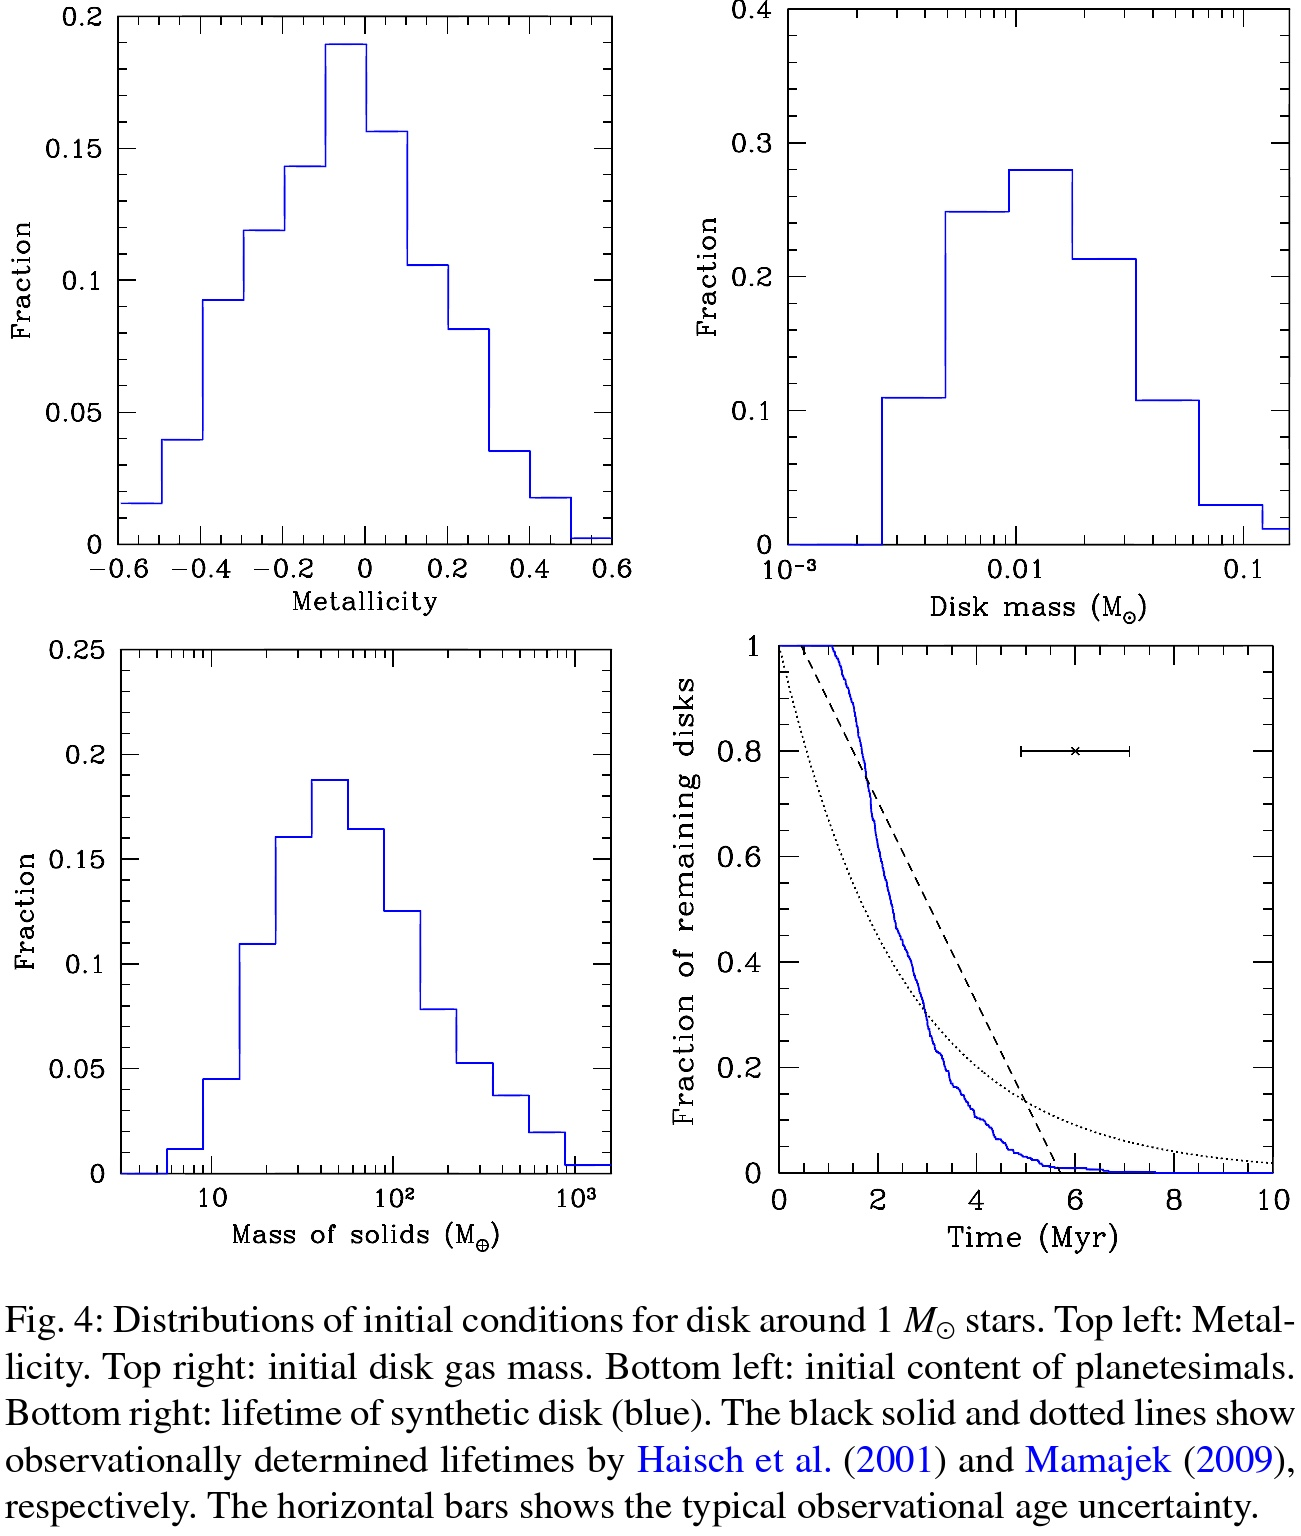
\includegraphics[keepaspectratio,width=\textwidth]{initdistro}\label{fig:initdistro}\caption{Da \cite{mordasini2018planetary}.}\end{figure}

\end{workout}

\begin{workout}[YSO: classificazione ]
SED: emissine a lunghezze d'onda millimetriche probano tutto il volume del disco, otticamente sottile a quelle lunghezze (Beckwith 90, Beckwith Sargent91).
$S_{\nu}\propto B_{\nu}(1-\exp{-\tau})\approx B_{\nu}\tau$: emission produced near cold disk mid-plane.
Rayleigh-jeans: $B_{\nu}\propto T$ and, since $\tau=\kappa\Sigma$, $S_{\nu}\propto \kappa\Sigma T$.
(SED: Andrews williams 07)
Survey: 0.3'', 345Ghz(870$\micro m$) 1Myr old Ophiuchus stars forming region
The absolute chronology and thermal processing of solids in the solar protoplanetary disk (Connelly Ivanova 12)
\end{workout}

\begin{workout}[Selfsimilar initial disk density solution]
Refs: Lynden-bel pringle 74
Se la viscosit\'a \'e statica e distribuita secondo $\nu\propto r\expy{\gamma}$:
\begin{align}
&R_c=R_1\mathcal{T}\expy{1/(2-\gamma)}\\
&M_d=M_{d,0}\mathcal{T}\expy{-1/2(2-\gamma)}\\
\end{align}
\end{workout}

\begin{workout}[Analitic disk model]
Chambers 09: On analytical model for the evolution of a viscous, irradiated disk
On location of snowline in protoplanetary disk (lecar chiang 06)
On the snow line in dusty PPD (Sasselov lecar 99)
Accretion disks around young object I: Detailed vertical structure (D'alessio Lizzano 98)
\end{workout}

\begin{workout}[YSO properties distro]
Refs: ''Protoplanetary Disk Structures in Ophiuchus''
da dove sono ricavete nei PPS?
mass: MMSN, andrews 10, manara 16
lifetime: IR/UV excess: haisch 01, mamajek 09
initial embryo starting position: relative spacing of few hill radii (kokubo ida 00), fill disk thinking of asyntituc isolation mass (Ida Lin 10), trapped (hasegawa pudritz 11, cridland 16)
Hueso 05: evolution of protoplanetary disk, meyer 06 Formation and evolution of planetary systems, Udry 07: statistical properties of exoplanets)
Distribuzione di probabilit\'a per condizioni iniziali.

Initial condition for planet formation (protoplanetry disk \cite{meyer2006formation}): disk metallicity, mass, lifetime, \ldots

{Metallicity and Dust/Gas}
$[M/H]$ distro modelled as normal: $\mu=-0.02$, $\sigma=0.22$ (photosphere of solar-like stars in solar neighborhood): Santos05.
$f_{dg}=f_{dg,\odot}10\expy{[M/H]}$ with $f_{dg,\odot}=0.01-0.02$.
\end{workout}

\begin{workout}[Classificazione YSO: convenzioni]
Sorgenti con SED declinante in mid infrared ($2.5-10\si{\micro\meter}$): $1.5<\alpha_{IR}=<0$. Active/passive: mass infall convert G into thermalradiation/reprocessed starlight.
Refs: Perrymann 10.3 - disk formation pg 218 - 
Classification based on slope of SED between $2-25\si{\micro\meter}$: $\alpha_{IR}=\TDly{\nu}{\nu F_{\nu}}=$ (Gail Hoppo 2010)
Spitzer: forming regions within 500pc
Formation: disk quickly forms as more distant material with high angular momentum, centrifugal radius $R(t)\propto\Omega^2 t^3$: . Class 0-I : protostellar disk, gravitational unstable (cloud collapse: the collapse of the cores of slowly rotating isothermal clouds, Terebey shu cassen 1984, selfsimilar collapse of isothermal spheres and star formation, shu 77). Singular isothermal sphere: $\rho=\frac{a^2}{2\pi G}r\expy{-2}$, $M(r)=\frac{2a^2}{G}r$
\end{workout}

\begin{workout}[Refs dischi protoplanetari]
Ciesla Dullemond10 
Perryman ch 10
williams cieza 11
Andrews 09-10
mamajek 2009 - Initial conditions of planet formation: lifetimes of primordial disks
infrared excess: gail hoppe10
\end{workout}


{\let\clearpage\relax\let\cleardoublepage\relax
\chapter{Schema di formazione planetaria per core accretion}
}

\begin{workout}[Refs GI vs CA]
planetesimal hypoithesis: chamberlin 05, Safronov 69, Hayashi 77. Formation on dynamical scale via GI: Kuiper 51, Cameron 62.
Core accretion o instabilit\'a gravitazionale?
La correlazione tra metallicit\'a del disco protoplanetario e il numero di pianeti (giganti) \'e in accordocon osservazioni?
\end{workout}


Lo schema di core accretion (CA) prevede la coagulazione della componente polverosa in embrioni planetari che, se abbastanza massicci sono in grado di accrescere il gas presente nel disco protoplanetario.

Lo schema di formazione considera l'instabilit\'a gravitazionale del disco.

Esistono alcuni dati osservativi in favore del primo modello:
\begin{itemize}
\item arricchimento dei pianeti del sistema solare rispetto a composizione solare di metalli (la composizione di Urano/Nettuno contiene $1\%$ di $H_2$, $He$ contenuto in pianeta di composizione solare con pari massa di metalli)
\item ipotizzando una successiva rimozione della parte gassosa il pianeta deve avere il tempo di sedimentare la componente metallica
\item \'e necessario un disco di massa solare e i pianeti si formerebbero a distanza maggiore
\item non spiega la formazione dei corpi minori
\end{itemize}

\section{Sedimentazione polvere e formazione planetesimi}

La polvere presente nel materiale interstellare ha dimensioni di \SI{0.1}{\micro\meter} sedimenta verso il centro del disco:

$F_D$ \'e la forza esercitata dal gas sulla particella di polvere
\begin{equation}
F_D=-\frac{1}{2}C_D\pi s^2\rho_gv^2
\end{equation}
nel caso cammino libero medio delle molecole di gas sia maggiore delle dimensioni della particella $C_D=\frac{8}{3}\frac{v_{th}}{v}$ (Epstein drag) per particelle pi\'u grandi \'e funzione del numero di Reynold.

L'equazione del moto per particella di polvere \'e
\begin{equation}
m_p\TDy{t}{v_z}=F_D-m_p\Omega^2z
\end{equation}
che risulta in condizioni stazionarie
\begin{equation}
v_{set}=\frac{\Omega^2}{v_{th}}\frac{\rho_d}{\rho_g(z)}sz
\end{equation}
Per particelle di \SI{1}{\micro\meter} tempo di sedimentazione \'e $\SI{2e5}{\year}$.
Inoltre turbolenza e coagulazione delle particelle hanno un ruolo non banale.
%t=mv/F
Inoltre la velocit\'a relativa tra gas e polvere causa un drift verso la stella massimo per particelle di \SIrange{0.01}{10}{\meter}  a \SI{1}{\astronomicalunit} per cui si deve avere rapida crescita oltre \SI{10}{\meter}.

Per passare a corpi di dimensioni kilometriche si ipotizzano 2 scenarii:
\begin{itemize}
\item La componente solida del disco di accrescimento sedimenta rapidamente in disco sottile: secondo il modello di Goldreich-Ward il disco di polvere \'e instabile e le condensazioni generano i planetesimi.
\item In assenza di sedimentazione la formazione procede tramite urti a 2 corpi e la turbolenza creando addensamenti, pu\'o accelerare la formazione di planetesimi.
\end{itemize}

\begin{workout}[refs planetesimal formation]
Armitage 07: lecture notes on formation and early evolution
 \end{workout}

\begin{workout}[Velocit\'a sedimentazione stzionaria]	
Grani piccoli raggiungono rapidamente la velocit\'a stazionaria di regime
\begin{equation}
v_{set}=\frac{\Omega^2}{v_{th}}\frac{\rho_d}{\rho_g(z)}sz
\end{equation}
 \end{workout}
 
\begin{workout}[Dust settling model]
weidenschilling 89: dust settling time
Dullemond dominique 04, johansen klahr 05, carballido 05, fromand papaloizou 06, turner 06,07
Furlan 06: Effects of dust growth and settling in T Tauri disks
Nomura 06: Dust Size Growth and Settling in a Protoplanetary Disk
\cite{lissauer1993planet}
 \end{workout}

\begin{workout}[Dust dynamics refs]
Weidenschilling cuzzi 06: Particle-gas dynamics and primary accretion, Apai Lauretta Protoplanetary Dust pg 100
Protoplanetary disk and their evolution pg 29
Protoplanetary dust: Apai Lauretta - particles dynamics pg 100
\end{workout}

\begin{workout}[Particle-gas dynamics. dust midplane sedimantation]
Weidenschilling cuzzi 06: Particle-gas dynamics and primary accretion, Apai Lauretta Protoplanetary Dust pg 100
Stopping time $t_s=\frac{\rho_sa}{\rho c_s}$ ($a<\lambda_g$). L'evoluzione dinamica delle particelle solide \'e determinata flussi macroscopici dovuti all'evoluzione del disco, gas-drag, settling
\end{workout}

\begin{workout}[Formazione planetesimi: meccanismo Goldreich-Ward]
Weidenschilling cuzzi 06: Particle-gas dynamics and primary accretion, Apai Lauretta Protoplanetary Dust pg 100
Stopping time $t_s=\frac{\rho_sa}{\rho c_s}$ ($a<\lambda_g$). L'evoluzione dinamica delle particelle solide \'e determinata flussi macroscopici dovuti all'evoluzione del disco, gas-drag, settling
\end{workout}

\section{Accrescimento planetsemi: formazione proto-pianeti.}


\begin{figure}[!t]
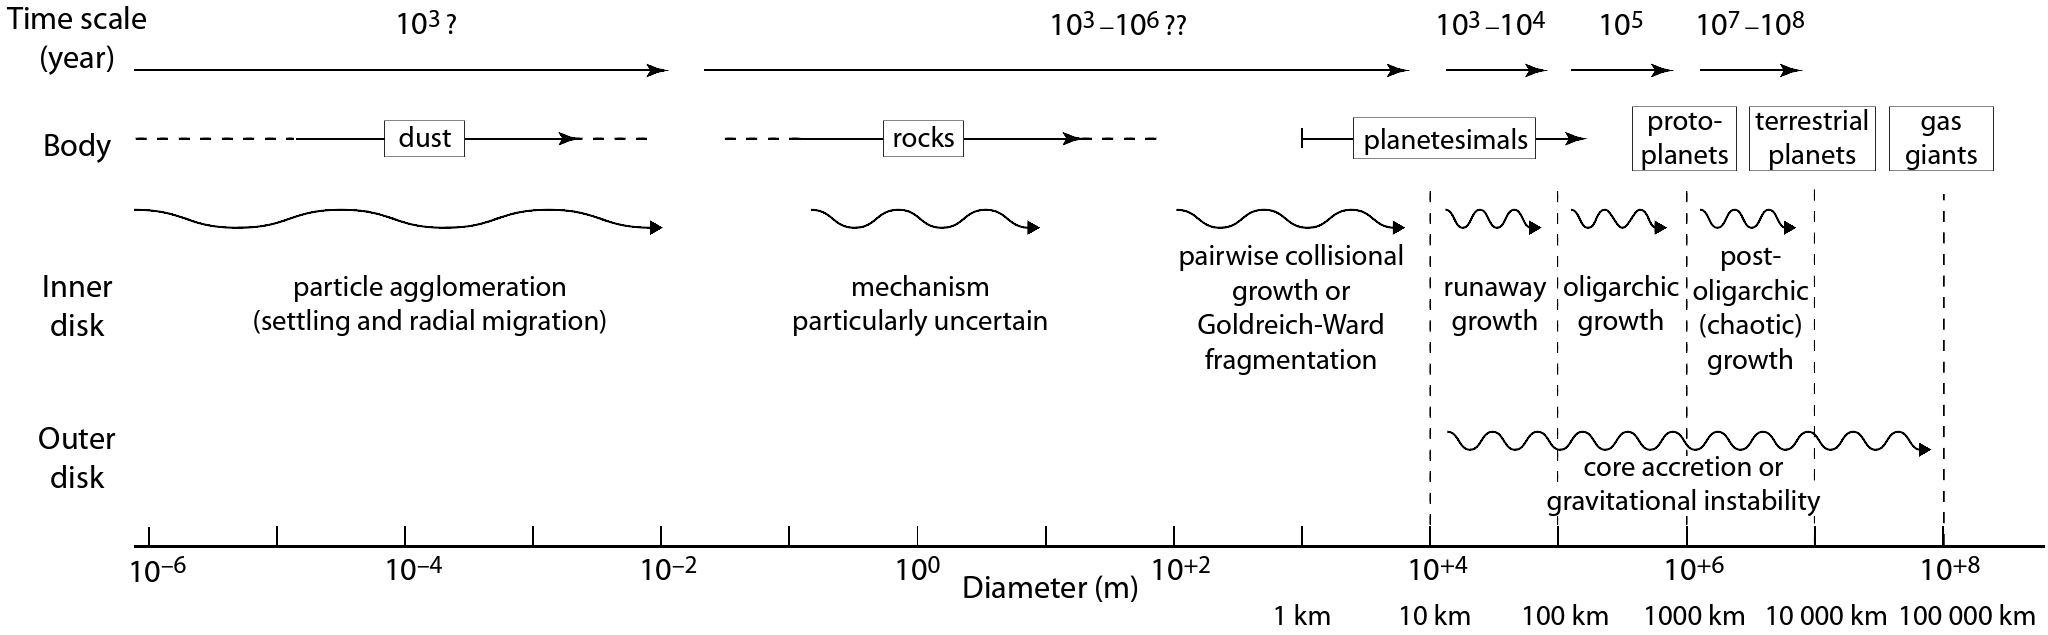
\includegraphics[width=0.9\textwidth]{accretiontimeline}
\end{figure}

\begin{workout}[Dynamical evolution of planetesimal swarm: refs]
Accretional evolution of planetesimal swarm (weidenschilling 97)
Goldreich 2004: Planet Formation by Coagulation: A Focus on Uranus and Neptune
Goldreich 04: FINAL STAGES OF PLANET FORMATION
rafikov 03: DYNAMICAL EVOLUTION OF PLANETESIMALS IN PROTOPLANETARY DISKS.
rafikov 02: The growth of planetary embryos: orderly, runaway, or oligarchic?
thommes 03: Oligarchic growth of giant planets
\end{workout}

\begin{workout}[10m-10km, 100km-1000km, 1000km-10000km: refs]
Lissauer pg 142-143
Perryman pg 226
\end{workout}

\subsection{Distribuzione planetesimi}

La popolazione dei planetesimi evolve attraverso interazione con gas e scattering/collisioni con planetesimi: l'interazione tra planetesimi trasforma il moto kepleriano in casuale e si ha equipartizione di energia tra pianetesimi di diversa massa; i planetesimi di massa minore hanno maggiore dispersione di velocit\'a, l'interazione col gas smorza eccentricit\'a e inclinazione inoltre due planetesimi hanno stessa velocit\'a relativa primo e dopo interazione ma aumenta la velocit\'a relativa al moto kepleriano in maniera casuale.

\'E ragionevole supporre che si arrivi rapidamente alla condizione $v>\Omega R_H$.

\begin{workout}[Planetesimal dynamics: viscous stirring]
The origin of anisotropic velocity dispersion of particles in a disc potential (Ida, Makino 93, Stewart-Wetherill 1988 Ida1990)
\end{workout}

\begin{workout}[Gravitational stirring: Viscous stirring and dynamical friction]
\begin{itemize}
\item Viscous stirring increses i,e
\item Dynamical stirring: tends to equalize energy of random motion among bodies having different masses and velocities
\end{itemize}
\end{workout}

\begin{workout}[orbital elements distribution: rayleigh distro]
I planetesimi hanno distribuzione di velocit\'a casuale, localmente equivalente a
\begin{equation}
f(e,i)=4\frac{\sigma}{m}\frac{ei}{\exv{e^2}\exv{i^2}}\Exp{[-\frac{e^2}{\exv{e^2}}-\frac{}{\exv{i^2}}]}
\end{equation}
\'e una distro gaussiana triassiale in coordinate cilindriche (Lissauer Stewart 93)
Lissauer pg 142-143
\end{workout}

\subsection{Regimi accrescimento dei protopianeti}

L'accrescimento di massa del protopianeta procede secondo
\begin{equation}
\TDy{t}{M_e}=\pi R_c\Sigma_p\Omega F_g
\end{equation}
$F_g$ \'e determinato dalla velocit\'a relativa tra proto-pianeta e planetesimi.

\begin{workout}[Protoplanets accretion of solids]
Other refs: Planet formation coagulation: focus on U,N (Goldreich 04), Final stages of planets formation (Goldreich 04), Formation of giant planets core: evaluating key processes (levison 09).
Safronov69: $\dot{M}_c=\Omega\Sigma_pR^2_{capture}F_G$, $R_{capture}$ larger than core radius due to gas drag, $F_G(e,i)$ gravitational focus (give rise to different growth regimes: runaway, oligarchic, orderly).
Runaway growth until protoplanets $100-1000km$ (dep on position).
Oligarchic growth: velocity of planetesimal raised by viscous stirring (gravitational scattering)/ damped by gas (until disk present).
Enhanced radius by atmospheric drag: Enhanced collisional growth of a protoplanet that has an atmosphere (Inaba Ikoma 03)
\end{workout}

\begin{workout}[orderly growth]
lissauer pg 144: equapartition effect saturation. This regime is never observed in simulations.
\begin{equation}
\frac{1}{m_p}\TDy{t}{m_p}\propto m_p\expy{-1/3}
\end{equation}
\end{workout}

\begin{workout}[runaway growth]
per planetesimi circa 1km (perch\'e?)
\begin{equation}
\frac{1}{m_p}\TDy{t}{m_p}\propto m_p\expy{1/3}
\end{equation}
\end{workout}

\begin{workout}[feeding zone]
Jacobi integral:
\begin{align}
&E_J=\frac{1}{2}(e^2+i^2)a^2\Omega^2-\frac{3}{8}b^2\Omega^2+\frac{9}{2}R_H^2\Omega^2\\
&\tilde{E}_J=\frac{E_J}{a^2h^2\Omega^2},\ h=R_H/a
\end{align}
Planetesimi con $\tilde{E}_J>0$ possono accrescere il protopianeta  cio\'e entro $w_{feed}=B_LR_H$, per orbite circolari $B_L=2\sqrt{3 }$.
\end{workout}

\begin{workout}[runaway to oligarchic. Isolation mass]
 NEW CONDITION FOR THE TRANSITION FROM RUNAWAY TO OLIGARCHIC GROWTH (Ormel 10)
 \begin{equation}
M_{iso}\propto M_*\expy{-1/2}\Sigma_p\expy{3/2}r^3
\end{equation}
$0.07\mearth{}$ 1AU, $9\mearth{}$ 5 AU.
Accretion among preplanetary bodies: runaway growth, summary of collision interactions
Understanding how planets become massive
\end{workout}
  
\begin{workout}[Accrescimento pianetesimi: orderly, runaway, oligarchic]
The growth of planetary embryos:  orderly, runaway, or oligarchic? (Rafikov 2002)
\begin{align}
\TDy{t}{M_e}\approx\pi R_e^2\Omega mN\frac{v}{v_z}[1+\frac{2GM_e}{R_ev^2}]
\end{align}
Accrescimento ordinato: $\frac{1}{M_e}\TDy{t}{M_e}\propto M_e\expy{-1/3}$. Accrescimento runaway: $\frac{1}{M_e}\TDy{t}{M_e}\propto M_e\expy{1/3}$. Accrescimento oligarchico: $\frac{1}{M_e}\TDy{t}{M_e}\propto M_e\expy{-1/3}$.
\end{workout}

\begin{workout}[Atmospheric drag increases accretion rate]

\end{workout}

\begin{workout}[Timescale of oligarchic growth]
kokubo ida 02 (ida lin 04)
\begin{align}
&\dot{M}_c=\frac{M_c}{\tau_c}\\
&\tau_c=\SI{1.2e5}{\year}(\frac{\Sigma_p}{\SI{10}{\gram\per\cubic\cm}})\expy{-1}(\frac{a_p}{\SI{1}{\astronomicalunit}})\expy{1/2}(\frac{M_p}{\mearth{}})\expy{1/3}(\frac{M_*}{\msun{}})\expy{-1/6}[(\frac{\Sigma_g}{\SI{2400}{\gram\per\cubic\cm}})\expy{-1/5}(\frac{a_p}{\SI{1}{\astronomicalunit}})\expy{1/20}(\frac{m}{\SI{e18}{\gram}})\expy{1/15}]^2
\end{align}
\end{workout}

\begin{workout}[Post-oligarchic growth: 1000km-10000km]
Chaotic growth until stable configuration is reached.
Factors determning orbital spacing: pg 229, earth formation (chambers 01, raymond 05, o'brian 06)
\end{workout}


{\let\clearpage\relax\let\cleardoublepage\relax
\chapter{Evoluzione struttura planetaria: accrescimento e fase isolata.}
}

\begin{workout}[Critical core mass]
From toward deterministic
\begin{equation}
M_{c,crit}\approx10(\frac{\dot{M}_c}{\num{e-6}\mearth{}\si{\per\year}})\expy{0.2-0.3}(\frac{\kappa}{\SI{1}{\square\cm\per\gram}})\expy{0.2-0.3}\mearth{}
\end{equation}•
\end{workout}

Se il core \'e sufficientemente massiccio lega il gas presente nelle disco: 
Seguendo \cite{rafikov2006atmospheres}.

Indico la massa di gas legata al core con
\begin{equation}
M_e=4\pi\int_{R_c}^{R_B}\rho(r')r'^2\,dr'
\end{equation}

dove $R_C$ \'e il raggio del core e il raggio di Bondi
\begin{equation}
R_B=G\frac{M_c}{c_0^2}\approx\SI{4e10}{\cm}a(AU)\expy{1/2}\frac{M_c}{\mearth{}}
\end{equation}
definito come raggio in cui energia termica e potenziale gravitazionale si equivalgono: il core perturba la pressione del gas del disco.

\section{Accrescimento idrostatico}

\begin{workout}[Wien displacement]
$\lambda_{max}T\approx \SI{3e-3}{\meter\kelvin}$
\end{workout}

\begin{workout}[Gas accretion: characterization of exoplanets from their formation]
\begin{align}
&E_t=E_g+E_i=\int_0^M\frac{Gm}{r}\,dm+\int_{M_z}^Mu\,dm=-\xi\frac{GM^2}{2R}\\
&-\TDof{t}E_t=L=L_M+L_R+L_{\xi}=\xi\frac{GM}{R}\dot{M}-\xi\frac{GM^2}{2R^2}\dot{R}+\frac{GM^2}{2R}\xi\\
\dot{M}=\dot{M}_Z+\dot{M}_{XY}
\end{align}
Mass conservation, hydrostatic equilibrium and energy transfer:
\begin{align}
&\TDy{r}{m}=4\pi r^2\rho\\
&\TDy{r}{l}=0\\
&\TDy{r}{P}=-\frac{Gm}{r^2}\rho\\
&\TDy{r}{T}=\frac{T}{P}&\TDy{r}{P}\nabla(T,P)\\
&\nabla(T,P)=\TDly{P}{T}=\min{(\nad{},\nrad{})}
\end{align}

Condizioni al bordo:
\begin{align}
&R=\frac{R_A}{1+R_A/(k_lR_H )},\ P=P_{neb}\\
&\tau=\max{(\rho_{neb}\kappa_{neb}R),2/3)},\ T_i^4=\frac{3\tau L_{int}}{8\pi\sigma R^2}\\
&T^4=T_{neb}^4+T_{int}^4,\ L(R)=L_{int}
\end{align}
$k_{liss}=3-4$, quindi $R_p\approx \min{(R_B,k_{liss}\expy{-1}R_H)}$.
\end{workout}

Rate di accrescimento limitato dalla velocit\'a di raffreddamento ($\tau\approx\tkh{}$):
\begin{align}
&\dot{M}_{XY}\propto,\ \frac{M_p}{M_*}<(H_P/R_p)^3/\sqrt{3}\\
&\dot{M}_{XY}\propto M_p
\end{align}

quindi la massa di gas aumenta esponenzialmente a partire da $M_c\approx10\mearth{}$.

\section{Instaurarsi instabilit\'a gravitazionale}

Se $H_p\approx R_p$ il pianeta perturba in maniera non trascurabile il disco (il rate di accrescimento di gas \'e maggiore di quello fornito dal disco). Il raggio del pianeta \'e determinato dalle condizioni al bordo per materia accresciuta tramite free-fall da $R_H$ a $R_p$:
\begin{align}
&\dot{M}_{XY}=\dot{M}_{XY,max},\ v_{ff}^2=2GM(\frac{1}{R}-\frac{1}{R_H})\\
&P=P_{neb}+\frac{\dot{M}_{XY}}{4\pi r^2}+\frac{2g}{3\kappa},\ \tau=\max{(\rho_{neb}\kappa_{neb}R,2/3)}\\
&T_{int}^4=\frac{3\tau L_{int}}{8\pi\sigma R^2},\ T^4=(1-A)T_{neb}^4+T_{int}^4
\end{align}


\begin{workout}[gas accretion refs]
Lissauer 09: Models of Jupiter’s growth incorporating thermal and hydrodynamic constraints
Rafikov 10: ''Constraint on giant planet production by core accretion''
Rafikov 04 Atmospheres of protoplanetary cores: critical mass for nucleated instability.
Refs: Planet formation models: the interplay with the planetesimal disc (Fortier 2013), Characterization of exoplanets from their formation I. Models of combined planet formation and evolution (Mordasini 12)
\end{workout}

\begin{workout}[Planet-Disk exchange in hydrodynamic manner]
Ormel 15/ Cimerman 17
\end{workout}

\section{Fase isolata}

fonti energia: tidal heating radiogeninc heat, star flux

{\let\clearpage\relax\let\cleardoublepage\relax
\chapter{Migrazione (e N-body interactions??)}
}

\begin{workout}[Migration refs]
Terquem papaloizou (planet formation and migration) pg 43
Planet-disk interaction and orbital evolution
Refs: \cite{ward1997protoplanet}, \cite{terquem2000disks}, \cite{menou2004low}, (
Planet-disk interaction and orbital evolution (kley Nelson 2012), 
Baruteau 2016)
crida06: On width and shape of gaps in PPD,crida phd, 
Trilling 98:Orbital evolution and migration of giant planet: modellingextrasolar planets (Angular momentum injection rate, torque from spinning star, Impact of planet migration models on planetary populations)
Dittkrist 14: Impact of planetsmigration models n planetarypopulation (Migration II inward/outward: non equilibrium gas flow, problem of isothermal disk migration timescale: migration I regime, Fig 7,
\end{workout}

\begin{workout}[planet locked in resonances]
as solar system satellites: goldreich 65.
N-body, resonanceand migration: The dynamics of two massive planets on inclined orbits (Veras Armitage 04)
orbital migration occurring at different rates due to disk parameters can produces convergent migration and locking into mean motion resonances.
kley 04
aligned absidal line: papaloizou 03
\end{workout}

\begin{workout}[type I: migration is too fast]
magnetic fields cloud produce stocasticity and thus s migration: nelson papaloizou 04, laughlin 04
laminar/turbulent disk: nelson 05 - tidal torque on fluctuations
global magnetic fields terquem 03
global distortion (non zero eccentricity): papaloizou 02
opaciy transitionmenou goodman 04
instabilities in inviscid gap enge: koller 03
\end{workout}

\begin{workout}[Width horseshoe region]
mordasini dittkrist14
\end{workout}

\section{Classificazione migrazione: risposta del disco e velocit\'a}

Il disco di accrescimento esercita momento torcente sul pianeta che produce un trasferimento di momento angolare dal pianeta al disco $\Lambda(a,R)$
\begin{align*}
&J=M_p\sqrt{GM_*a_p}\\
&\TDy{t}{a}=2a_p\frac{\Gamma_t}{J}=-(\frac{a}{GM_*})(\frac{4\pi}{M_P})\int_{r_{int}}^{r_{out}}r\Lambda\Sigma\,dr
\end{align*}
$r_{int}, r_{out}$ inner/outer disk radius (rif to disk ar planet)


\begin{workout}[M14:type I]
below few tenth of $\mearth{}$.
Linblad torque: inside/outside corotation region.
corotation torque: depends on thermodynamics regime of interaction between planet/disk.
\end{workout}

\begin{workout}[Corotation torque: non-linear (except early stages) horseshoe drag.]
(On horseshoe drag of low-mass planets)
Jump in angular momentum of particles undergoing U turn, before/after planets (in librating orbit).
ward91, masset 01,02, masset papaloizou 03, paardekooper papaloizou 09.
Linear analysis: corotation torque arise from anulus of radial extent H around corotation, launch of evanescent waves in coorbital region; horseshoe analysis consider horseshoe region.
\end{workout}

\begin{workout}[Horseshoe drag]
Horseshoe drag low-mas planet: migration in isothermal disk (casoli Masset 09): torque, width of corotation region
\end{workout}

\begin{workout}[type I: planets not massive enough to open a gap]
Linear response of disk to orbiting planets - perturbazione del pianeta sul disco si propagano come onde di densit\'a fuori dalle risonanze e come onda evanescente fra le risonanze nella regione di corotazione. Il protopianeta esercita un momento torcente sulle onde di densit\'a cha assieme  a quello di corotazione \'e responsabiledello scambio di momento angolare tra disco mkoto orbitale del pianeta: la maggior parte del toque \'e esercitato vicino alle risonanze di L./corotazione dove la lunghezza d'onda della perturbazione \'e lunga (lontano la perturbazione ha lunghezza d'onda breve: contributo mediato a zero): terquem00.
Il momento pu\'o essere calcolato facendo una analisi lineare delle onde eccitate in 2D/3D o sommando i momenti torcenti puntiformi esercitati alle risonanze di lindblad/corotazione.
\begin{align}
&t_I\propto J/\dot{J}\propto(H/a)^2\\
&t_e\propto e/\dot{e}\propto(H/a)^4
\end{align}
\end{workout}

\begin{workout}[type III and coorbital torque]
COnsidero un pianeta migrante: quando il gap \'e parziale materiale percorre l'orbita ed esercita momento t, positive/negative feedback.
Per un pianeta che migRA VERSO L'ESTERNO SI HA
$2\pi\Sigma R\TDy{t}{R}$ \'e il flusso di massa che impartisce momento per unit\'a di massa al protopianeta quando la materia attraversa la regione di corotazione di spessore w, $w\omega/2$: con $w=2H$ si ha
\begin{align}
F_{cr}=2\pi R\Sigma\omega^2 H^2\frac{1}{c_s}\TDy{t}{R}=1/2M_d\omega\TDy{t}{R}\\
F_{crb}=-1/2M_b\omega\TDy{t}{R}
\end{align}
dove la seconda \'e inerzia (??) massa legata al pianeta.
quazione del moto:
\begin{equation}
1/2M_pa\omega\TDy{t}{a}=1/2(M_d-M_b)a\omega\TDy{t}{a}+T_{ext}
\end{equation}
\end{workout}

\begin{workout}[M14:type II and outward migration]
adiabatic and local isothermal disk: pardekooper 10/11
Type II planet-dominated for mass $100\mearth{}$.
$\dot{a}_p\propto v_g$: ??
Veras armitage 04 (exoplanets with $a>20au$): outward migration seldom important, radius velocity reversal when type II migration occure $R_{mvc}$ is outside them.
\end{workout}


\section{Migrazione tipo I: regime lineare}

\begin{workout}[Lindblad/corotation torque: linear]
Unperturbed disk: axisymmetric, keplerian rotation $\Omega(r)=\sqrt{GM_*/r^3}$, vanishing radial velocity. Planet potential, periodic in $\phi$, $\phi_p=\Omega_pt$:
\begin{align*}
&\psi_p(r,\phi,t)=-\frac{Gm_p}{|\vec{r}_p(t)-\vec{r}|}=\sum_{m=0}^{\infty}\psi_m(r)\cos{m[\phi-\phi_p(t)]}
\end{align*}
Total torque excertes by disk on planet
\begin{equation*}
\Gamma_t=-\int_{disk}\Sigma(\vecp{r}{F})\,df=\int_{disk}\Sigma(\vecp{r}\wedge\nabla\psi_p)\,df=\int_{disk}\Sigma\PDy{\phi}{\psi_p}\,df
\end{equation*}
$\Sigma$ surface density,  $\vec{F}$ specific force, $df$ surface element.
Whenever frequency of individual potential component as seen by fluid particle in disk $\omega=m(\Omega(r)-\Omega_p)$, matches a natural  oscillation frequency of the disk we have resonant condition: torques are calculated at resonant locations.
Lindblad (due to m-component of planet potential) and corotation torques:
\begin{align*}
&\Gamma_m^L=\left.\sign{(\Omega-\Omega_p)}\frac{\pi^2\Sigma}{3\Omega\Omega_p}(r\TDy{r}{\psi_m}+\frac{2m^2(\Omega-\Omega_p)}{\Omega}\psi_m)^2\right|_{r=r_L}\\
&\Gamma_m^C=\left.\frac{m\pi^2}{2}\frac{\psi_m}{r\TDy{r}{\Omega}}\TDof{r}(\frac{\Sigma}{B})\right|_{r=r_C}
\end{align*}
Differnetial Lindblad torque
$B=\frac{\kappa^2}{4\Omega}$ is the second Oort constant and represents z component of flow vorticity $\nabla\wedge\vec{v}|_z$
\end{workout}

\begin{workout}[Migration I in isothermal disk: pressure. Adiabatic, irradiated?]
Low mass planet in isothermal disk: linear analysis of perturbed flow.
When pressure can't be neglected the resonance condition becomes $m(\Omega(r)-\Omega_p=\sqrt{\kappa^2(r)(1+\xi^2)}$ where $\xi=\frac{mc_s}{\Omega r}$ where we used isothermal sound speed and let $c_s=H\Omega$: for $m\to\infty$ L. res position becomes $r_L=r_p+\frac{2H}{3}$ (torque cutoff).

Linear. Occur if $R_H$ is smaller then H, disk scale heigth, and if viscous torque are dominant compared to gravitational torque.
Subtypes: locally isothermal, adiabatic, un/satured-corotation torque: cooling behaviour of gas (Baruteau masset08, Casoli masset 08, paardekooper10,kley 09); timescales: dittkrist 14.
Migration timescale in isothermal approx (ida lin 08 a:):
\begin{align*}
&\tau_I=\frac{1}{2.728+1.082p_{\Sigma}}(\frac{c_s}{a_p\Omega})^2\frac{M_*}{M_p}\frac{M_*}{a_p^2\Sigma_g}\Omega\expy{-1}\\
s&\dot{a}_p=-\frac{a_p}{\tau_I}
\end{align*}
Paardekooper10, Dittkrist14: total torque $\Gamma_t=\frac{1}{\gamma}(C_0+C_1p_{\Sigma}+C_2p_T)\Gamma_0$ where $C_i$ depends upon sub-regime.
Benitez Llambay 15: heating torque, Paardekooper14 Pierens 15: dynamic corotation torque.
\end{workout}

\section{Massive enough planet to open gap: migration II}


\begin{workout}[Planetary torque: nonlinear regime, type II, gap formation]
Lin papaloizou 79: at conjuction with planets a fluid element trajectory is deflected in frame centered with planet by angle
\begin{equation}
\beta=\arctan{\delta v/v}=\arctan{(\frac{GM_p}{bv_0^2})}
\end{equation}
$v_0$ velocit\'a relativa fluido-pianeta; dopo l'interazione l'elemento di fluido \'e in orbita ellittica attorno alla stella
\begin{figure}[!t]
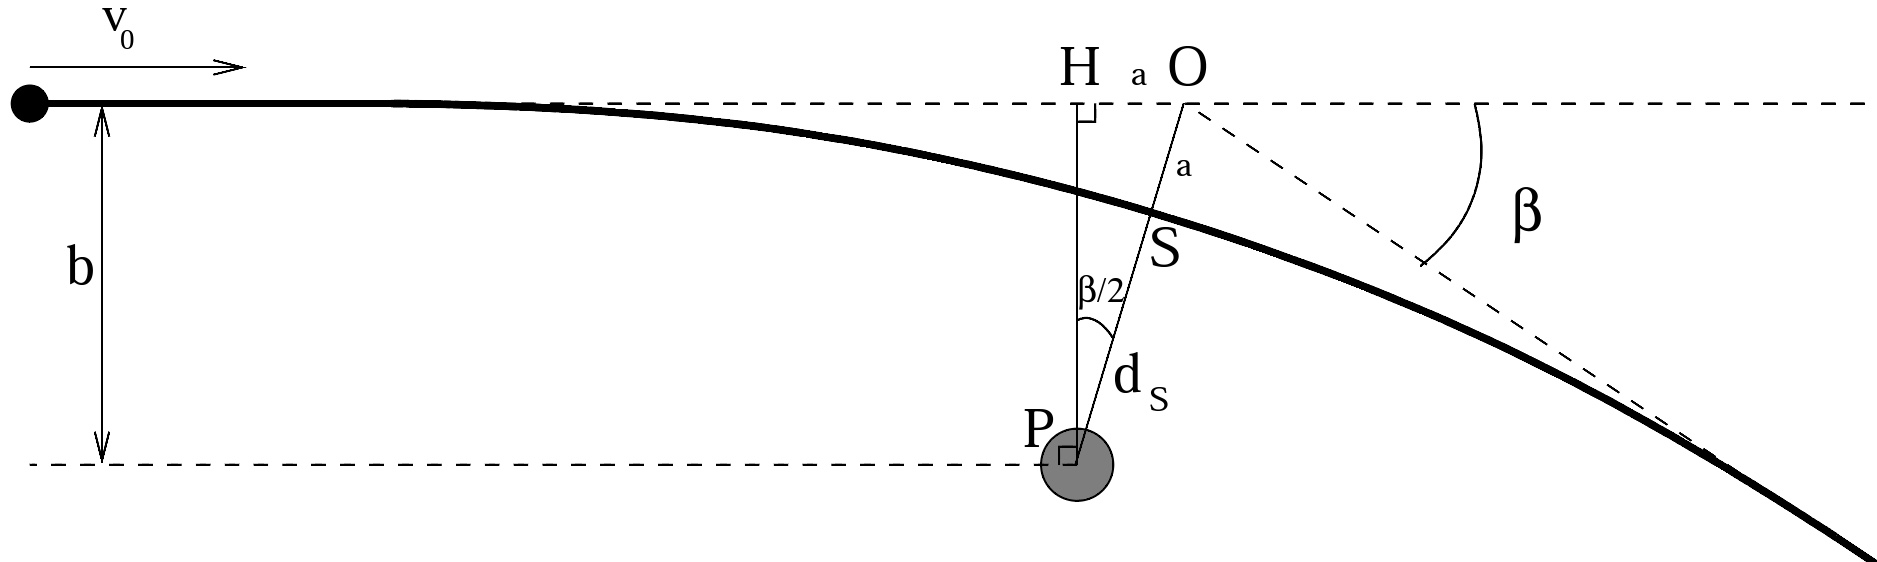
\includegraphics[width=0.9\textwidth]{impulseapprox}
\end{figure}
Qual \'e il trasferimento di momento angolare disco-pianeta associato a quest'interazione?
Trasferimento di momento per unit\'a di massa:
\begin{align}
&\Delta u=u(1-\cos{\delta})\approx u\delta^2/2\\
&\Delta J=au\delta
\end{align}
lungo direzione del originale di moto del protopianeta.
Pe rmateria in orbita circolare interna/esterna al pianeta il trasferimento \'e positivo/negativo.
(The interaction is frictional with interior speeding up protoplanet while exterior slowing down; viscous interaction with disk return mass element in circular orbit)
Il calcolo esatto che tiene conto del fatto che siamo in SR rotante (LP93) introduce fattore correttivo $K_0=4/9[2K_0(2/3)*K_1(2/3)]^2$.
La velocit\'a relativa \'e $u=a|\Omega_p-\Omega_g$ e dato che l'interazione avviene vicino al pianeta $|\Omega_p-\Omega_g|\approx3/2b\Omega_p/a$.
Rate trasferimento momento angolare tra interno del disco e pianeta
\begin{equation}
\TDy{t}{J}=\int_{b_{min}}^{+\infty}a\Sigma\Delta J|\Omega_p-\Omega_g|\,db
\end{equation}
Per disco esterno all'orbita l'espressione \'e la stessa con segno invertito perch\'e il disco or a \'e pi\'u lento del protopianeta.
Il parametro d'impatto minimo \'e l'assunzione implicita di un gap nel disco a assenza di materia nella regione di corotazione (discussione applicabilein regime non-lineare)
Formazione gap: perch\'e il gap si stazionario il momento scambiato nell'interazione disco-pianeta deve essere almeno quello trasportato dal moto viscoso del disco:
\begin{equation}
\TDy{t}{J}|_{visc}=3\pi\nu\Sigma a^2\omega
\end{equation}
deve essere quindi $\TDy{t}{J}|_{visc}<\TDy{t}{J}$
Cut-off: $b_{min}\approx H$, la pressione smorza effetti su scala pi\'u piccola; regime non-lneare, richiesto per gap formation, lunghezza-scala del flusso non minore di $r_H$: predndendo $b_m=2r_h$ si ha
\begin{equation}
\frac{M_p}{M_*}>\frac{40\nu}{a^2\omega}
\end{equation}
Formazione di gap per dischi tipici sopra massa di saturno.
Migrazione tipo II: il pianeta prende momento dal disco esterno (dovuto al flusso viscoso) e cede quello richiesto al disco esterno dal trasporto viscoso: normalmente il bilancio \'e negativo quindi il pianeta migra verso l'interno.
Quando la massa del pianetaa non eccede la massa locale del disco il tempo scale di migrazione \'e
\begin{equation}
t_{II}(yr)=\frac{1}{3\alpha}(\frac{a}{H})^2\Omega\expy{-1}=0.05/\alpha(a/H)^2(a/au)\expy{3/2}
\end{equation}
per $H/a\approx0.1$, $\alpha=\numrange{e-3}{e-2}$ a $a=1-5 au$ si ha $t_{}=10^3-10^4yr$.
\end{workout}

Refs: On the tidal interaction between protoplanets and the primordial solar nebula. II - Self-consistent nonlinear interaction (1986)
Non-linear. For larger planet mass, when disk density distro is changed cons., the linear hteory is no more adeguate. If angular momentum isdeposited locally (viscous dissipation/shock waves)  the disk receeds from planets
Ida-lin04: angular momentum trasport in viscous accretion disk without planets that in type II migration act as relays that transmit angular momentum at that rateacross their gap via tidal torques.
Alibert05: the planet follow the gas except when massive than local disk.
Duffell14, Durmann kley 15: questioning that migration II follows viscous evolution of the disk but due to torque??


Planet-disk interactions: exchange of angular momentum. Low mass planet-linear theory.(''Planet-disk interactions and orbital evolution'')
Low mass planets: Lindblad and corotation torque. Rapid migration of intermediate mass planets. Gap forming massive planets: slower migration determined by viscous evolution of disk. (Role of disk self-gravity and MHD turbulence as function of planet mass).


\section{Migrazione III:}
Planet-disk interactions: exchange of angular momentum. Type III migration: planet of intermediate mass. (‘’Planet-disk interactions and orbital evolution’’).

Flow-through corotation torque: $\Gamma_{flow}=2\pi\Sigma_s\dot{a}_p\Omega_pa_p^3x_s$.

\begin{align*}
&\dot{a}_p=\frac{2\Gamma^L}{\Omega_pa_p(m_p’-\delta m)}
\end{align*}

\section{Eccentricity and inclination evolution}
Planet-disk interactions: normal, tangential, radial forces. eccentricity and inclination evolution. (‘’Planet-disk interactions and orbital evolution’’)
Decomposition of planet’s potential: non-circular orbit
\begin{align*}
&\psi_p(r,\phi,t)=-\frac{Gm_p}{|\vec{r}_p(t)-\vec{r}|}=\sum_{m=0}^{\infty}\sum_{n=-m}^m\psi_{m,n}(r)\cos{m\phi+(n-m)\Omega_pt]}
\end{align*}

Eccentricity damping.
For each m,n there are 3 resonant locations: external L resonance act to increase, corotation res. to damp (if unsaturted), and coorbital L res damp $e_p$. Linear analysis for low mass planets indicates rapid exponential damping of $e_p$:
\begin{align*}
&\TDy{t}{e_p}\propto-e_p,\ \tau_e\approx(\frac{H}{r})^2\tau_{mig}\\
&e_P>\frac{H}{r}: \TDy{t}{e_p}\propto-e_p\expy{-2}
\end{align*}
Risultati analoghi per inclinazione.	

\section{Altre interazioni che producono migrazione}

\begin{workout}[planet overlflowing roche lobe migrate outward]
trilling 98:n During mass flow planet moves outward to conserve angular momentum
\end{workout}

\begin{workout}[Other (than?) types of migration]
planet-planet scattering (rasio ford 96, kozai (nagasawa 08, tidal interactions with gas disk (goldreich tremaine 80, tanaka 02))
\end{workout}


{\let\clearpage\relax\let\cleardoublepage\relax
\chapter{N-body interactions inside proto disk}
}
\cleartorecto

{\let\clearpage\relax\let\cleardoublepage\relax
\part{Modelli di formazione globali}
}
Lo scopo dei modelli di formazione globali \'e di costruire una descrizione semplificata dei processi fisici che portano alla formazione di un pianeta; quindi generare una popolazione planetaria a partire da distribuzione di condizioni iniziali, del disco di accrescimento, ricavata dalle osservazioni che riproduca la distribuzione di caratteristiche osservate, tenendo conto dei bias osservativi.

{\let\clearpage\relax\let\cleardoublepage\relax
\chapter{Modelli di formazione globali e semplificazioni introdotte}
}

\begin{workout}[Ref PPS]
Towarddeterminist model of planetary formation iV: effectsof type I migration
									: accumulation neare iceline
									: dynamical intaraction and coagulation of multiple rocky embrios (isolation mass, semi-analytic vs n-body)
									: eccentricity distribution of gas giant
Theoretical models of planetary system formation: mass vs. semi-major axis	(alibert carron 13)			Lecture 15 -planetary ...
Modelling planetary system formation with N-body simulation (11)
Global model of planet formation and evolution
Planetary population synthesis
planet population synthesis					
\end{workout}

\section{Modello disco di accrescimento e distribuzione condizioni iniziali}

Refs: Sec4 mordasini09

La popolazione planetaria \'e costruita risolvendo un modello di formazione planetaria pi\'u o meno realistico a partire da condizioni iniziali distribuite per rispecchiare le osservazioni e determinate da argomenti teorici.

\begin{workout}[modello globale: evoluzione dal semplice al complesso]
Global model of planets formation and evolution: more detailed submodels
\end{workout}

Il modello pi\'u semplice di disco di accrescimento usa distribuzione esponenziale per andamento densit\'a superficiale e temperature, assumendo disco otticamente sottile, e relazione $L_*\propto M_*^4$ di sequenza principale. Le lacune di questo modello sono che i dischi sono otticamente spessi con transizioni nell'opacit\'a, non \'e presente evoluzione temporale consistente.

Modelli pi\'u recenti  risolvono l'equazione per l'evoluzione viscosa:
\begin{align}
&\TDy{t}{\Sigma}=\frac{1}{r}\PDof{r}[3r\expy{1/2}\PDof{r}(\nu\Sigma r\expy{1/2})]+\dot{\Sigma}_w(r)+\dot{\Sigma}_p(r)\label{eq:diskaccrphev-m18}\\
&\dot{\Sigma}_w(a)=\left\{\begin{array}{c}0\\\frac{\dot{M}_w}{2\pi(a_{max}-R_g)a}\\\end{array}\right.
\end{align}
con $\dot{\Sigma}_w$ contributo della foto-evaporazione,  $\dot{\Sigma}_p$ contributo di accrescimento di gas dei pianeti e con densit\'a superficiale iniziale:
\begin{equation}
\Sigma(a,t=0)=\Sigma_0(\frac{r}{1AU})\expy{p_g}\Exp{[-(\frac{r}{R_o})\expy{2+p_g}]}(1-\sqrt{\frac{r}{R_i}})
\end{equation}
in i parametri possono essere scelti casualmente secondo una distribuzione di probabilit\'a ricavata dalle osservazioni.

La distribuzione di massa e la frazione di dischi protoplanetari per ammassi stellari di et\'a diversa \'e mostrata in \ref{fig:initdistro}: la massa \'e determinata misurando flusso di emissione termica della polvera la distribuzione di $\log{M_{disk}}$  \'e gaussiana e per il cluster Ophiuchus la distribuzione \'e fittata da gaussiana con $\mu=-1.38$ ($M_{disk}=0.042\msun{}$) e $\sigma=0.49$.

Il tempo caratteristico del disco \'e determinato dalla viscosit\'a $\alpha$: fissata $\alpha$, e assumendo la distribuzione uniforme nel logaritmo di $\dot{M}_w$, e calcolando  $t_{disk}(\alpha,\Sigma_0,\dot{M}_w)$ si determinano gli estremi dello fotoevaporazione per riprodurre tempi di vita osservati.

 $t_{disk}(\alpha,\Sigma_0,\dot{M}_w)$ per $\dot{M}_w=\SIrange{5e-10}{3e-8}\msun{}/\si{\year}$ per $\alpha=\num{7e-3}$.

\begin{workout}[viscosit\'a disco]
Nella popolazione planetaria simulata $\alpha$ \'e fissato sulla base delle osservazioni  ed \'e omogeneo e costante.
\end{workout}

\begin{workout}[Modello di disco di accrescimento - (Mordasini18: 4) - Introduzione descrizione fenomeni grazie a PPS]
Refs: garaud lin 07, chiang goldreich 97
Un modello di disco  di accrescimento usato nelle simulazioni considera l'evoluzione della densit\'a superficiale tramite l'equazione \eqref{eq:diskaccrphev-m18}
\begin{align}
&\TDy{t}{\Sigma}=\frac{1}{r}\PDof{r}[3r\expy{1/2}\PDof{r}(\nu\Sigma r\expy{1/2})]+\dot{\Sigma}_w(r)+\dot{\Sigma}_p(r)\label{eq:diskaccrphev-m18}\\
&\dot{\Sigma}_w(a)=\left\{\begin{array}{c}0\\\frac{\dot{M}_w}{2\pi(a_{max}-R_g)a}\\\end{array}\right.
\end{align}
Densit\'a superficiale iniziale:
\begin{equation}
\Sigma(a,t=0)=\Sigma_0(\frac{r}{1AU})\expy{p_g}\Exp{[-(\frac{r}{R_o})\expy{2+p_g}]}(1-\sqrt{\frac{r}{R_i}})
\end{equation}
4-Mordasini18 (Hayashi81). $p_g\approx1$ (Andrews10).
\end{workout}

\section{Distribuzione iniziale planetesimi ed evoluzione}

Assumendo conversione completa di polvere in planetesimi, la densit\'a superficiale di planetesimi \'e
\begin{equation}
\Sigma_p(t=0,r)=f_{dg}\eta_{ice}\Sigma_g(t=0,r)
\end{equation}
con $f_{dg}$ rapporto gas/polvere (circa metallicit\'a) \'e una parametro casuale con distribuzione che riflette distribuzione di metallicit\'a stellari, $\eta_{ice}$ tiene conto della discontinuit\'a nella distribuzione superficiale di solidi all'iceline.

Sulla scorta della piccola differenza tra composizione solare e composizione meteoritica e assumendo inoltre che il ferro sia un buon indicatore della componente solida  si usa la formula
\begin{equation}
\frac{f_{D/G}}{f_{D/G\odot}}=10\expy{[\cel{Fe}{}{}{}/\cel{Fe}{}{}{}]}
\end{equation}

\begin{workout}[Planet host stars are enriched in nikel and silicon]
Robinson06
\end{workout}

Si introduce un fattore correttivo per il drift della polvere entro i \SI{20}{\astronomicalunit} compreso tra $2-4$ e infine si sfrutta la distribuzione della metallicit\'a per stelle di massa solare nelle vicinanze del Sole:
\begin{equation}
p([Fe/H])=\frac{1}{\sigma\sqrt{2\pi}}\exp{-\frac{([Fe/H]-\mu)^2}{2\sigma^2}}
\end{equation}
Per le stelle campionate da CORALIE si ha $\mu=-0.02$ e $\sigma=0.22$.

L'evoluzione della distribuzione dei planetesimi tiene conto dell'acrescimento sugli embrioni planetari:
\begin{equation}\dot{\Sigma}_p=-\frac{(3M_*)\expy{1/3}}{6\pi a_p^2B_LM_p\expy{1/3}}\dot{M}_c\end{equation}
e generalmente si assume che eccentricit\'a e inclinazione seguono distribuzione di Rayleigh.

Il drift dei planetesimi dovuto all'interazione col gas e la formaziane gap nella distribuzione dei planetesimi sono di solito trascurati.

\begin{workout}[Initial planetesimal distro]
Dust converted early everywhere fully-efficient (mordasini18: pg 12),Thommes pg8)
\begin{align*}
&\Sigma_p(t=0,r)=f_{dg}\eta_{ice}\Sigma_g(t=0,r)\\
&\dot{\Sigma}_p(r)=-\frac{1}{2\pi aB_LR_H}\dot{M}_c
\end{align*}
Icelines Mordasini 1141: inside where T exceeds sublimation
{Embryo starting position}
Usually a distro uniform in log(a): relative spacing of few Hill spheres (Kokubo Ida 10)
Ida, lin10: asymptotical isolation mass ''Toward a Deterministic Model of Planetary Formation VI'',
Trapped evolution model: Hasegawa pudritz 11, Cridland 16
\end{workout}

\section{Caratteristiche iniziali degli embioni planetarii e accrescimento}

La massa iniziale dei core deve essere molto minore della massa di isolamento: si usano core di frazioni di massa terrestre; la distanza dalla stella varia seguendo distribuzione di probabilit\'a $p(a)$ inversamente proporzionale alla distanza orbitale $p(a)\,da\propto\frac{da}{\Delta}\propto\,d\log{a}$. Il momento di comparsa \'e determinato dal rate di accrescimento dei planetesimi \eqref{eq:Gaccretionpl}.

La massa dei core varia per l'accrescimento dei planetesimi secondo
\begin{align}
&\dot{M}_c=\Omega\Sigma_pR^2_{capt}F_G
%&\dot{\Sigma}_p(r)=-\frac{1}{2\pi aB_LR_H}\dot{M}_c
\end{align}

Per determinare l'accrescimento di gas \'e necessario calcolare la struttura planetaria in alternativa si pu\'o averne una stima da
\begin{align}
&\dot{M}_{e,KH}=\frac{M_p}{\tau_{KH}}\\
&\tau_{KH}=10\expy{p}(\frac{M_p}{\mearth{}})^q(\frac{\kappa}{\si{\gram\per\square\cm}})\si{\year}
\end{align}
dove p,q sono ottenuti tramite modelli di struttura planetaria
\begin{workout}[Higher mass gap formation reduces accretion rate]
\begin{equation}
f_{va04}=1.668(\frac{M_p}{\mjupiter{}})\expy{1/3}\exp{-\frac{M_p}{1.5\mjupiter{}}}+0.04
\end{equation}
\end{workout}

\subsection{Parametrizzazioni della migrazione}

\begin{workout}[Migrazione mordasini 09]
La velocit\'a di migrazione calcolata per disco isotermo (\cite{tanaka2002}) \'e troppo rapida
\end{workout}


\begin{workout}[model migration-pps]
Tanaka02-m09
Paardekooper 11 - Dittkrist 14
\end{workout}

\begin{workout}[Lindblad torque: velocit\'a migrazione I]
masset casoli 10/paardekooper 10
\end{workout}

\begin{workout}[type I/type II transition]
m09: Hill radius larger than disk scale hight
\end{workout}

\begin{workout}[Saturation mass of horseshoe drag]
eq 2: theimportance of disk structure in stalling planet migration
\begin{equation}
\TDy{t}{r}=f(p,q,p_{\nu},p_{\xi})\frac{M_p}{M_*}\frac{\Sigma r^2}{M_*}(\frac{r\Omega}{c_s})^2r\Omega
\end{equation}
\end{workout}

\begin{workout}[Velocit\'a tipo II: viscosit\'a]
disk dominated
planet dominates: $\TDy{t}{a}=-\frac{3\nu}{a}\frac{\Sigma(a,t)a^2}{M_p}$
\end{workout}



\section{popolazioni sintetiche}
%Considero i risulati di alcuni modelli di formazione planetari (\cite{mordasini2018planetary}). 
La soluzione delle equazioni che descrivono l'accrescimento di massa dei protopianeti e la loro evoluzione orbitale interata su numerose combinazioni delle condizioni iniziali produce una popolazione di sistemi planetari appena formati dal disco-protoplanetario.

\begin{workout}[Diagramma $(a-M)$]

\begin{figure}[!ht]
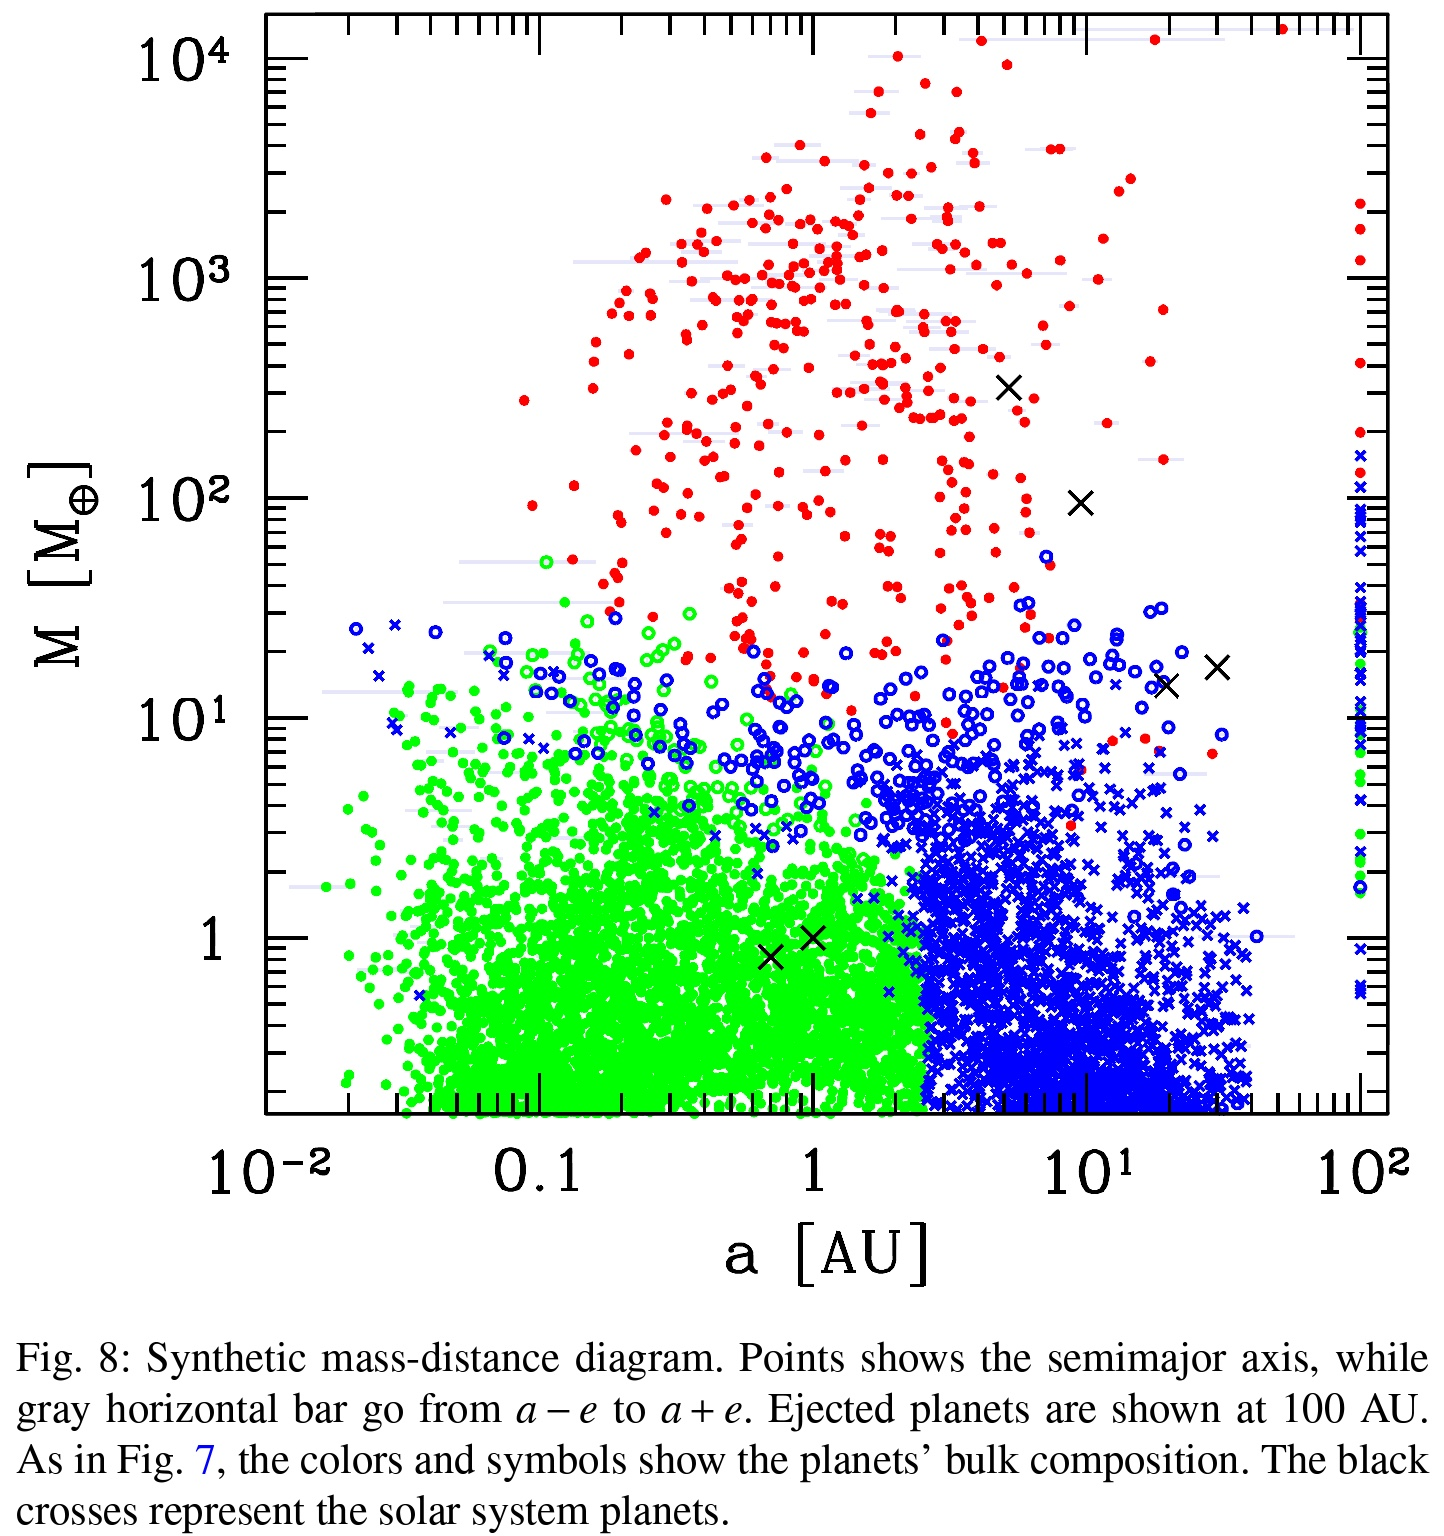
\includegraphics[trim={0cm 12cm 0 0},clip, width=0.9\textwidth,keepaspectratio]{ma-synth}
\caption{Da \cite{mordasini2018planetary}. Simulazione popolazione planetaria di 504 sistemi Punti rossi: pianeti giganti con $M_e/M_c>1$; blu hanno accresciuto core oltre la iceline, verdi all'interno dell'iceline .}
\end{figure}

La distribuzione della popolazione planetaria \'e mostrata in \ref{fig:MaLR-freq-synth}: la posizione finale di un pianeta \'e terminata principalmente dalla posizione iniziale e dai tempi caratteristici di accrescimento e migrazione; considerando inoltre l'interazione gravitazionale tra i pianeti si hanno effetti delle risonanze e eccitazione eccentricit\'a.

\begin{figure}[!ht]
\begin{subfigure}[b]{0.47\textwidth}
\centering
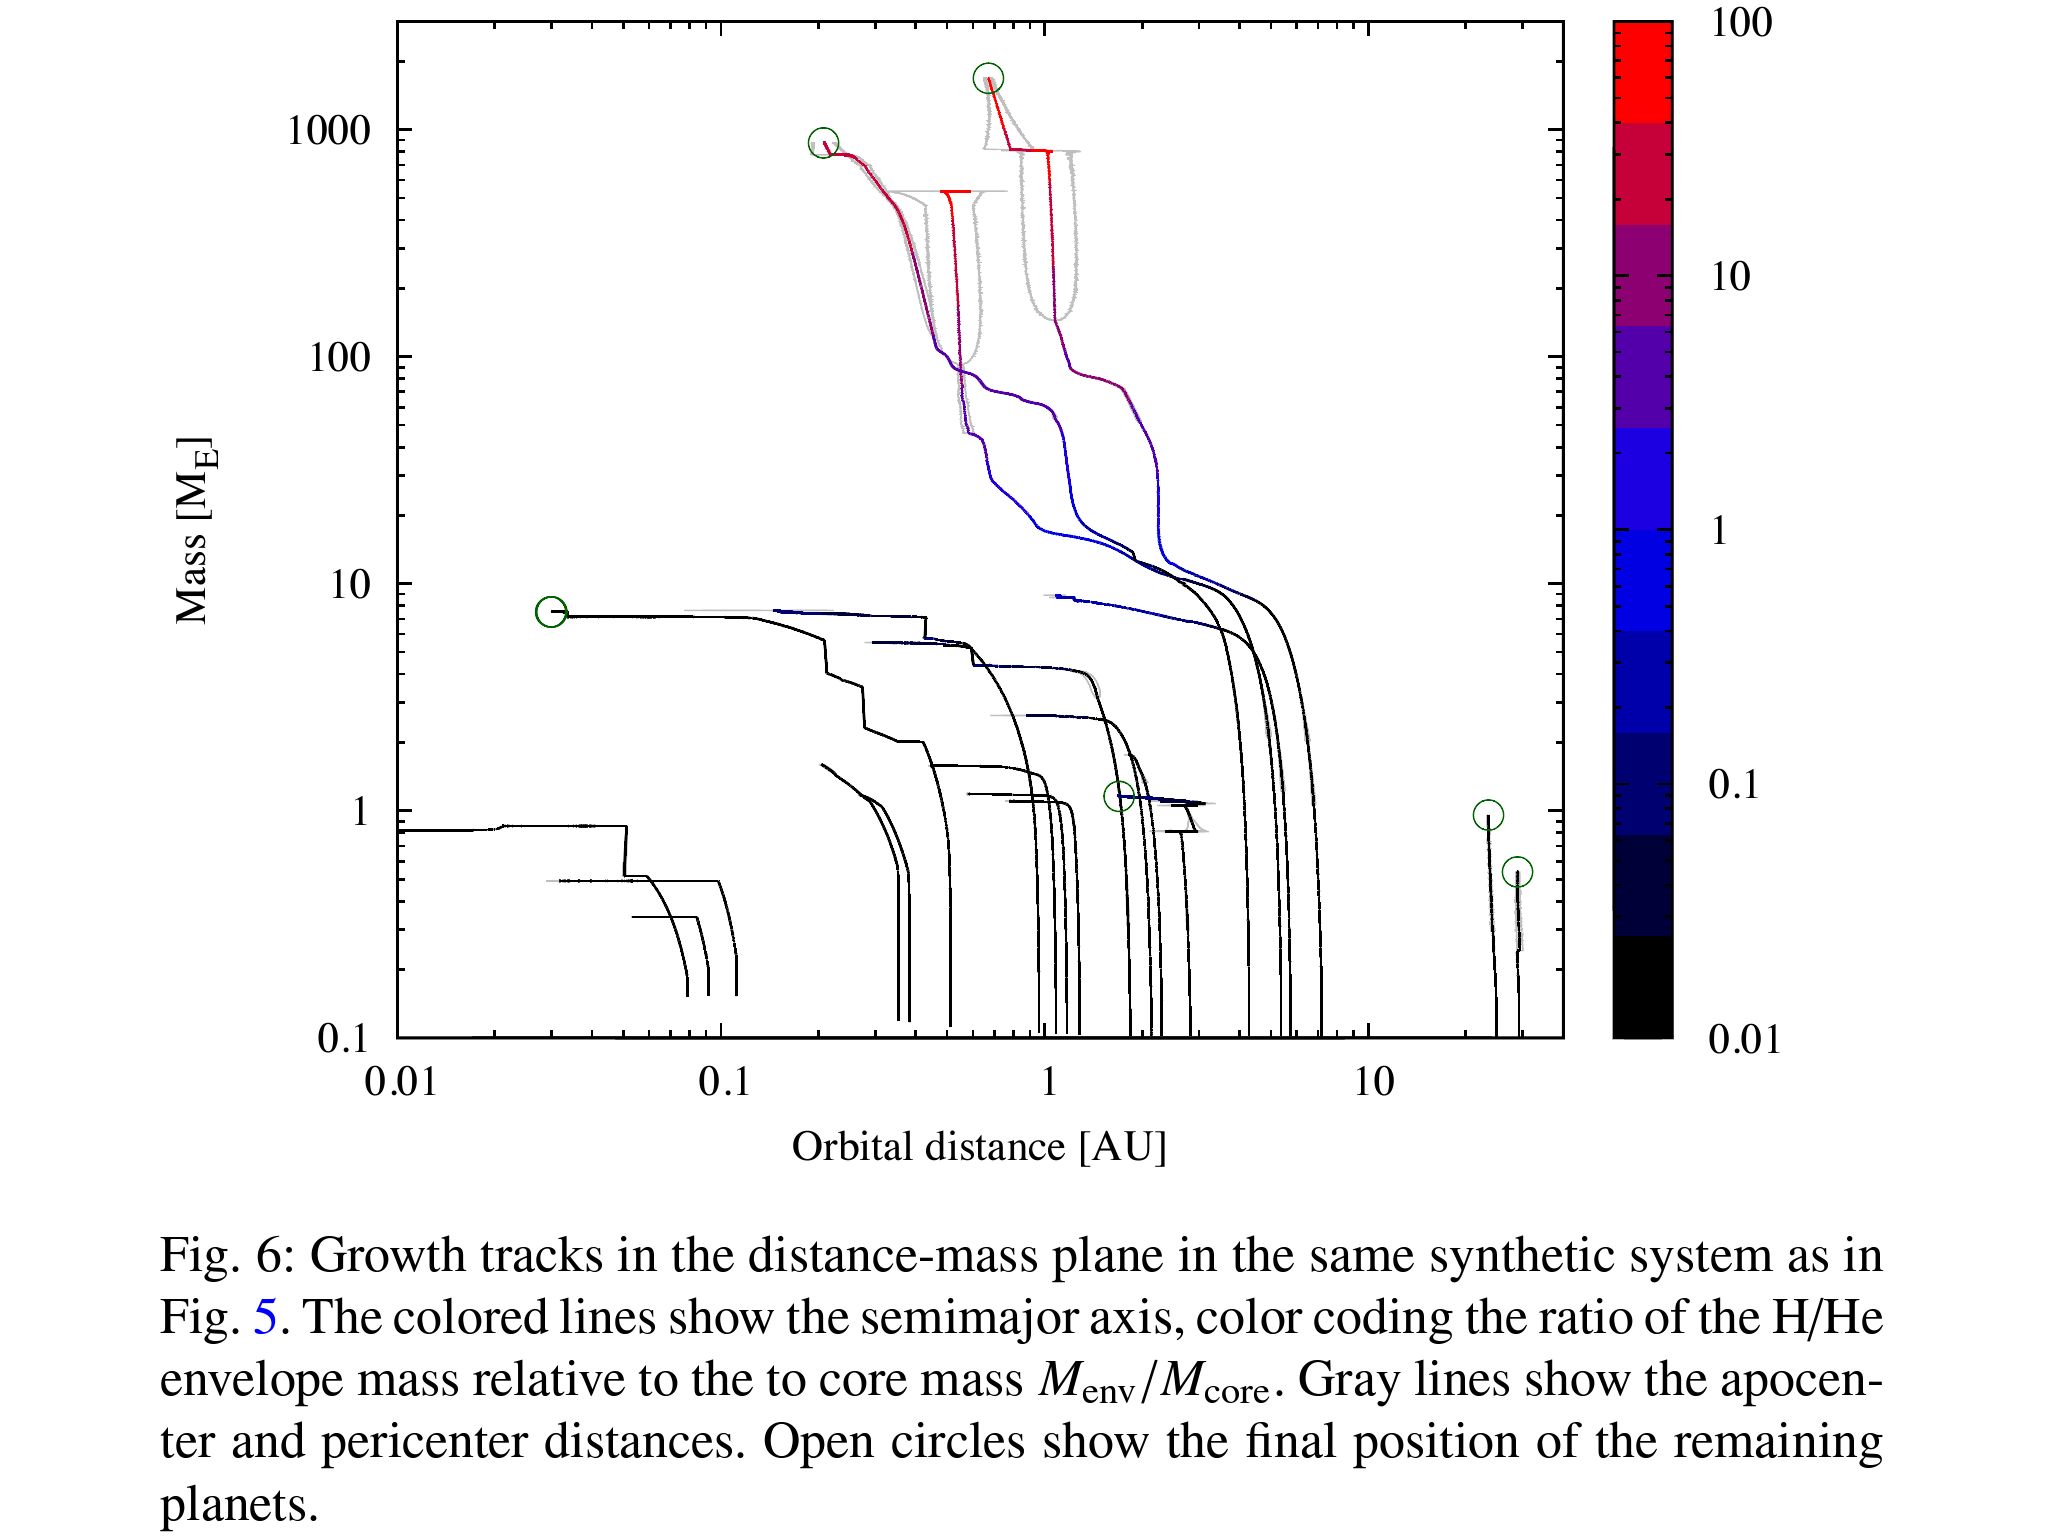
\includegraphics[trim={0cm 12cm 0 0},clip, width=0.9\textwidth,keepaspectratio]{track1}
\caption{Da \cite{mordasini2018planetary}. Formazione di un sistema planetario nel diagramma $a-M$: alla scomparsa del disco protoplanetario si hanno 2 pianeti giganti, un nettuniano caldo e 3 pianeti terrestri. La scala di colore indica la composizione $\frac{M_e}{M_c}$.}\label{fig:track1}
\end{subfigure}
~
\begin{subfigure}[b]{0.47\textwidth}
\centering
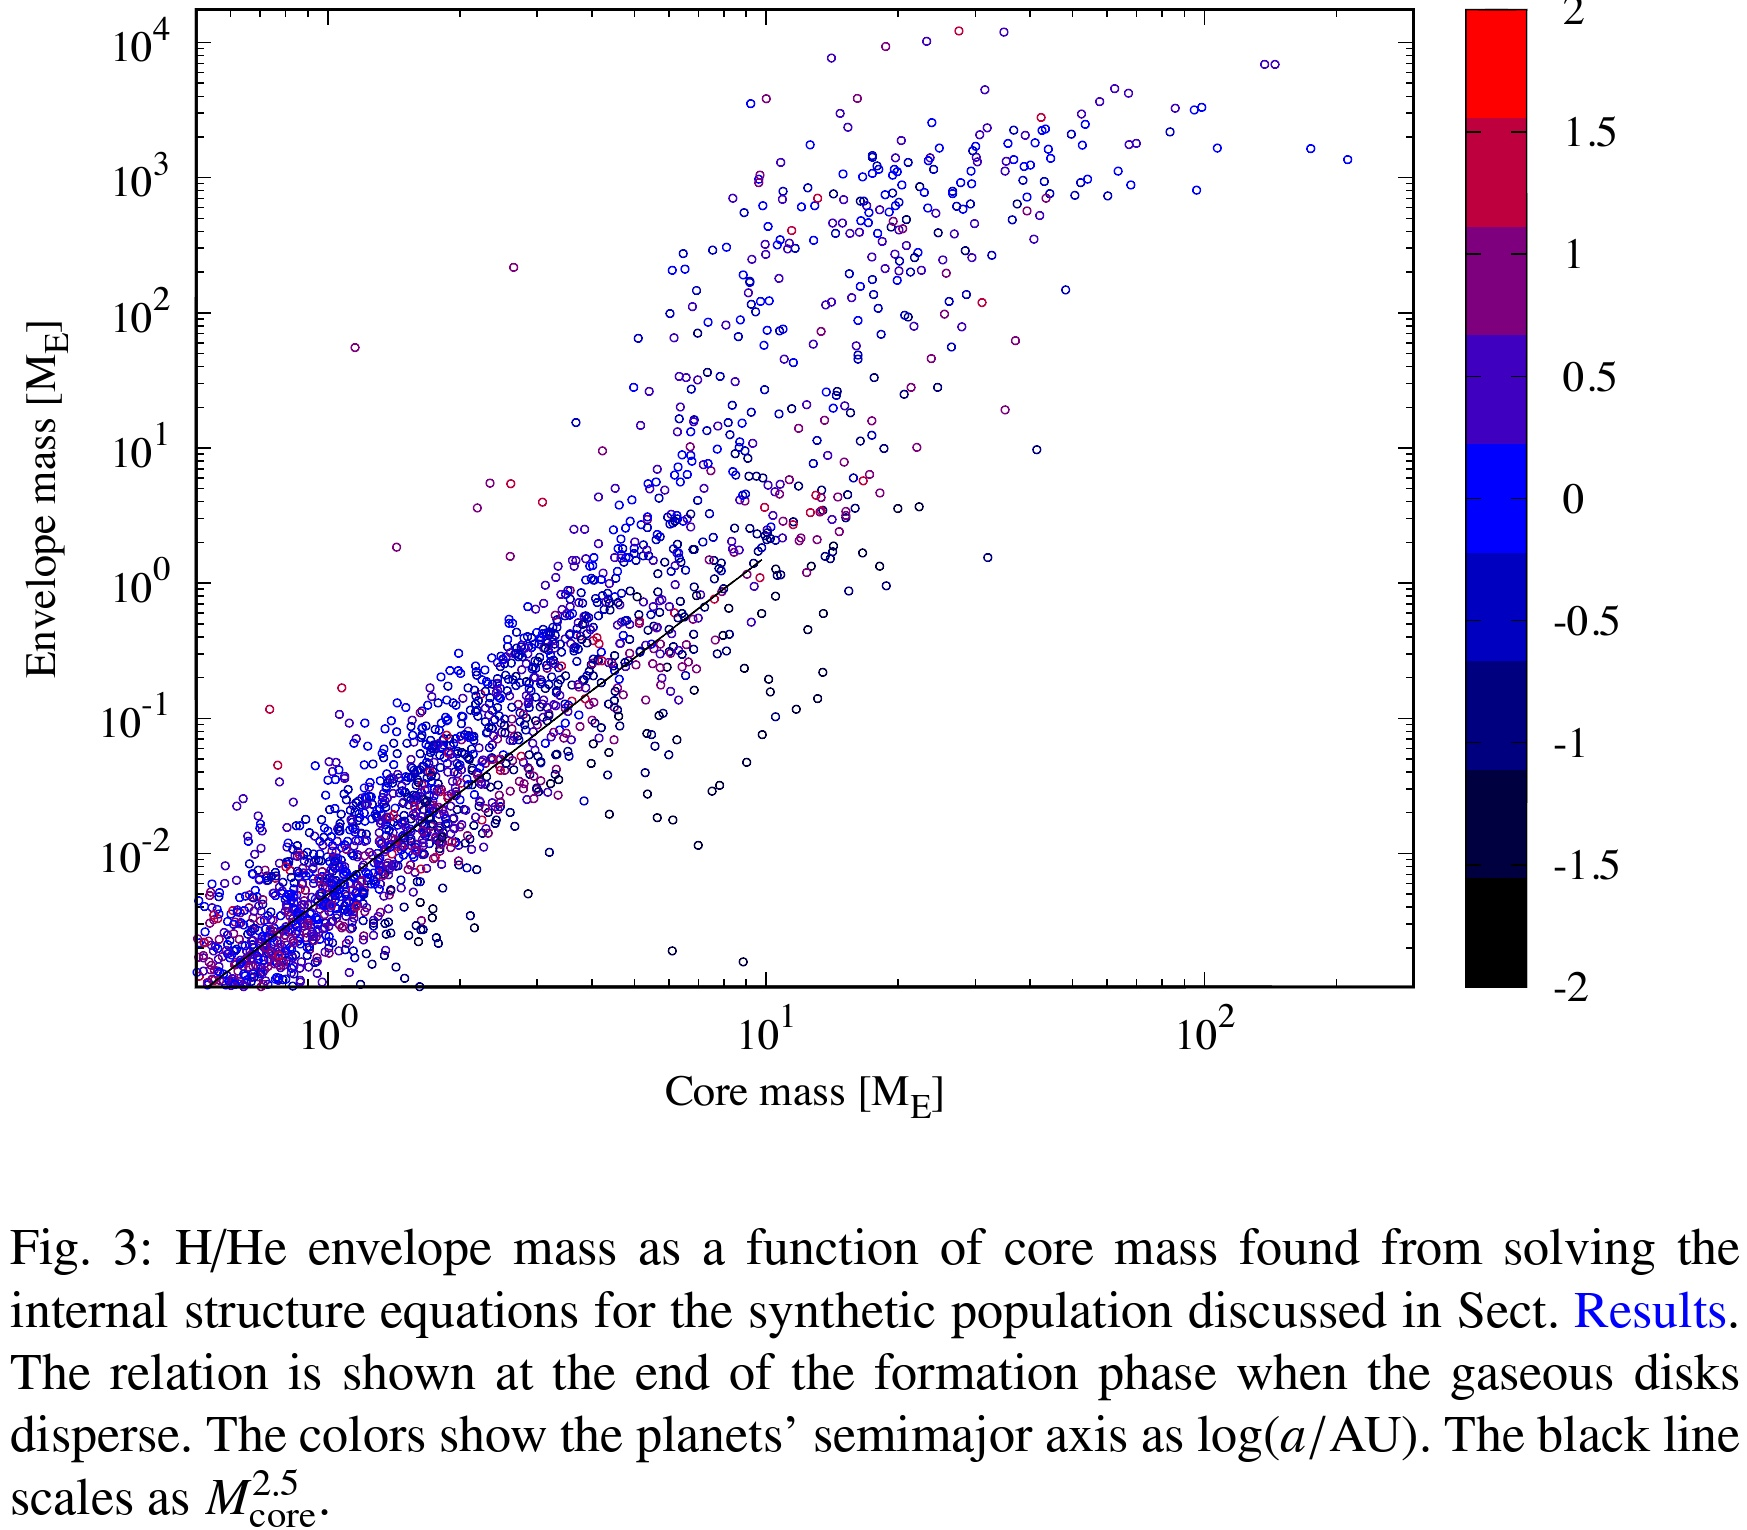
\includegraphics[trim={0cm 12cm 0 0},clip, width=0.9\textwidth,keepaspectratio]{envelopecoresynth}
\caption{Da \cite{mordasini2018planetary}. }
\end{subfigure}
\end{figure}

Differenze con osservazioni.

Popolazione pianeti in origine nettuniani (frazione giaccio nel core $50\%$) che migrano all'interno accumulando materiale roccioso (frazione ghiaccio nel core $10-20\%$): saturazione momento di corotazione positivo.

\end{workout}
\begin{itemize}
\item Numerosi sistemi con piccola massa
\item Sistemi pianeti di piccola massa e giganti: sweet spot per pianeti giganti \'e all'esterno dell'ice-line.
\item Un pianeta gigante superstite di scattering trapianeti gignti vicini. Sistemi rari formati in dischi massicci con alta metallicit\'a
\end{itemize}



\begin{figure}[!ht]
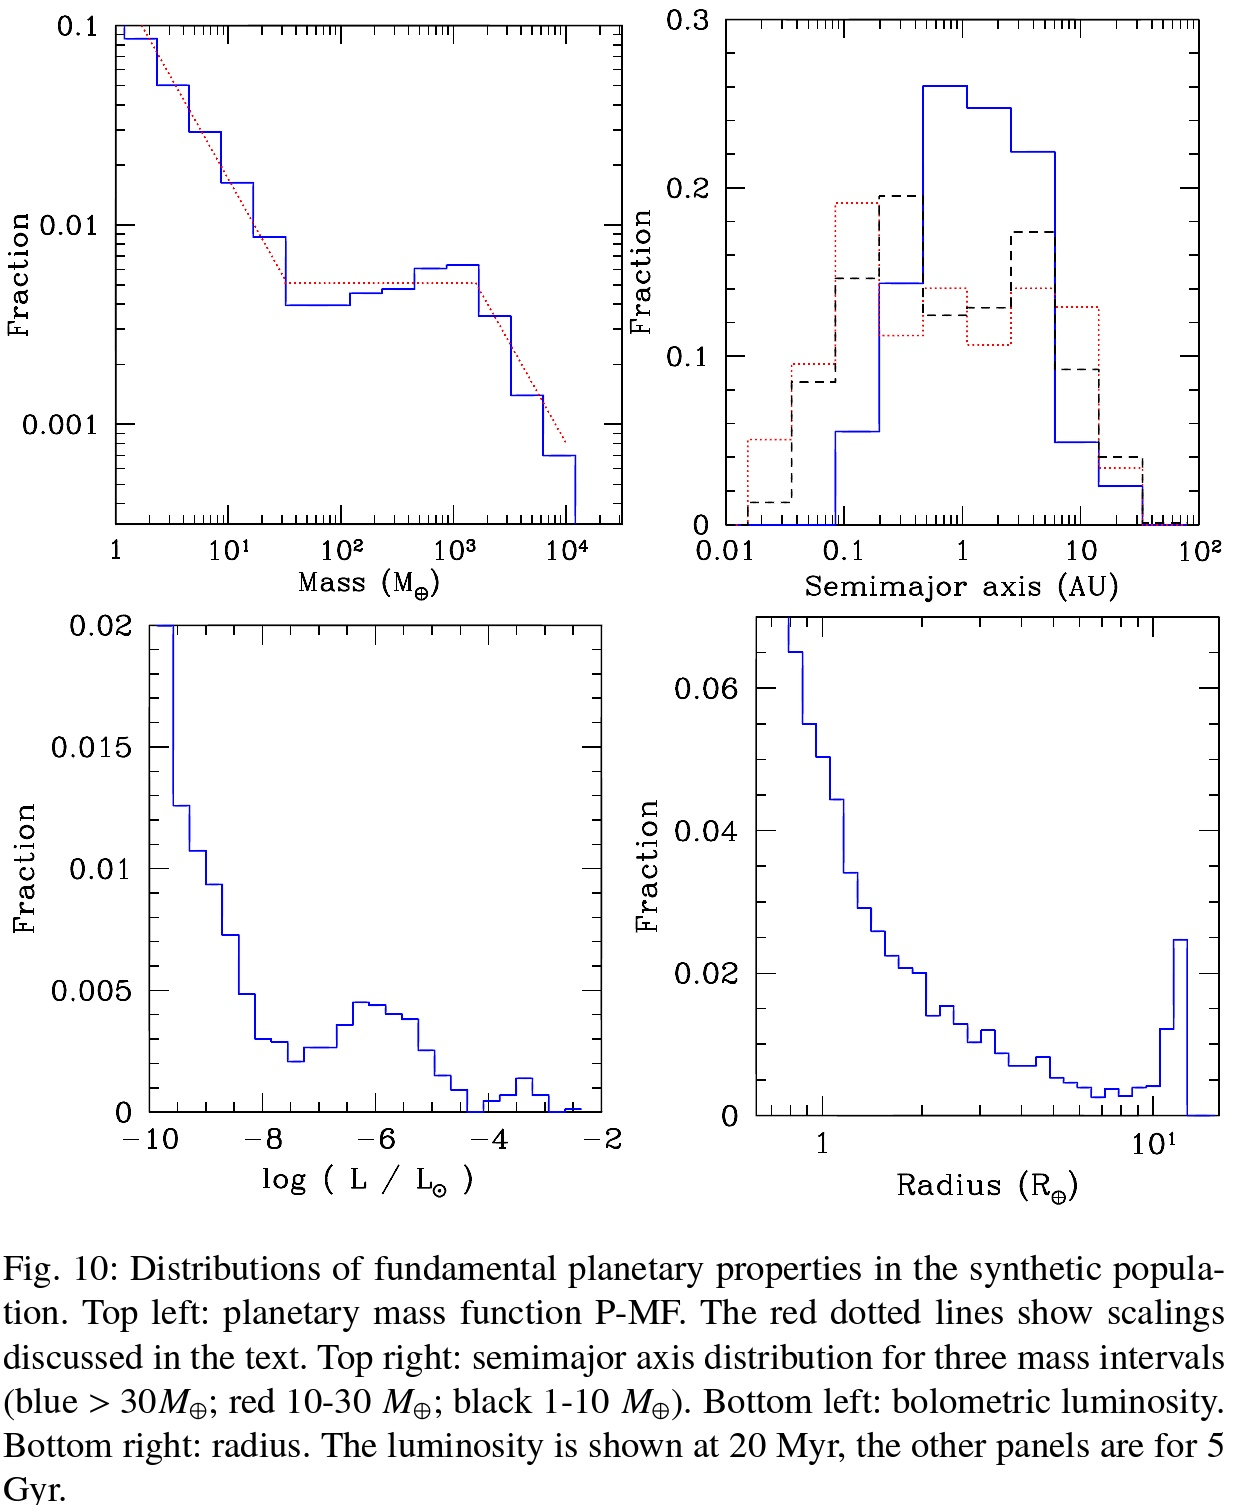
\includegraphics[trim={0cm 10cm 0 0},clip, width=0.9\textwidth,keepaspectratio]{MaLR-freq-synth}\label{fig:MaLR-freq-synth}
\caption{Da \cite{mordasini2018planetary}. }
\end{figure}

\subsection{Caratteristiche delle distribuzioni delle propriet\'a fisiche dei pianeti e significativit\'a}

La \ref{fig:MaLR-freq-synth} mostra la distribuzione di massa di 509 pianeti della popolazione sintetica di \cite{mordasini2018planetary}: la distribuzione della massa dei pianeti mostra due andamento diversi per pianeti fino a $30\mearth{}$ formati da solidi e pianeti che hanno raggiunto la massa critica peravviare l'accrescimento di gas runaway. La differente slope della distribuzione di massa nelle due regioni caratterizza i differenti meccanismi di accrescimento. 

\begin{workout}[Distro luminosit\'a: relazione M-L]
La distribuzione di luminosit\'a segue andamento $L\propto M^2$ con terzo picco per innesco deuterio a $\log{\frac{L}{\lsun}}\approx-3.5$
\end{workout}

La distribuzione del raggio dei pianeti mostra picco a $1\rjupiter$ e crescita per piccoli raggi dovuta al loro lungo $\tkh{}$ e quindi scarso accrescimento di H/He.

La distribuzione dei semi-assi cresce rapidamente tra $0.01-0.1\si{\astronomicalunit}$, resta uniforme in log tra $0.1-10\si{\astronomicalunit}$ nonostante molti pianeti migrino all'interno,mentre i pianeti giganti sono ristretti in \SIrange{0.1}{6}{\astronomicalunit}.

{\let\clearpage\relax\let\cleardoublepage\relax
\chapter{Confronto semi-quantitativo tra caratteristiche popolazioni sintetiche e osservate}
}

Per confrontare una popolazione planetaria simulata con le osservazioni \'e opportuno, oltre a tenere conto dei bias osservativi, valutare per quali sottoinsiemi dell'ensamble di pianeti ossevati le approssimazioni fatte nel modello sono valide.

\section{Struttura orbitale e tipo di pianeta}

\begin{table}
\begin{tabular}{|ccc|}
\hline
N&Giganti ($M>300\mearth{}$)&vicini ($P\leq100\si{\day}, R\geq\rearth{}$)\\
\hline
1&4.8&8.4\\
2&7.4&12.8\\
3&5.4&11.4\\
4&0.4&10.0\\
$\geq5$&0.0&11.4\\
$\exv{S}$&18.0&54.0\\
O&10-20&50-60\\
\hline
\end{tabular}
\caption{Percentuale di stelle con N pianeti del dato tipo nella popolazione sintetica di \cite{mordasini2018planetary} e confronto con osservazioni.}
\end{table}

Nettuno/Saturno in posizioni poco affollate


\begin{figure}[!ht]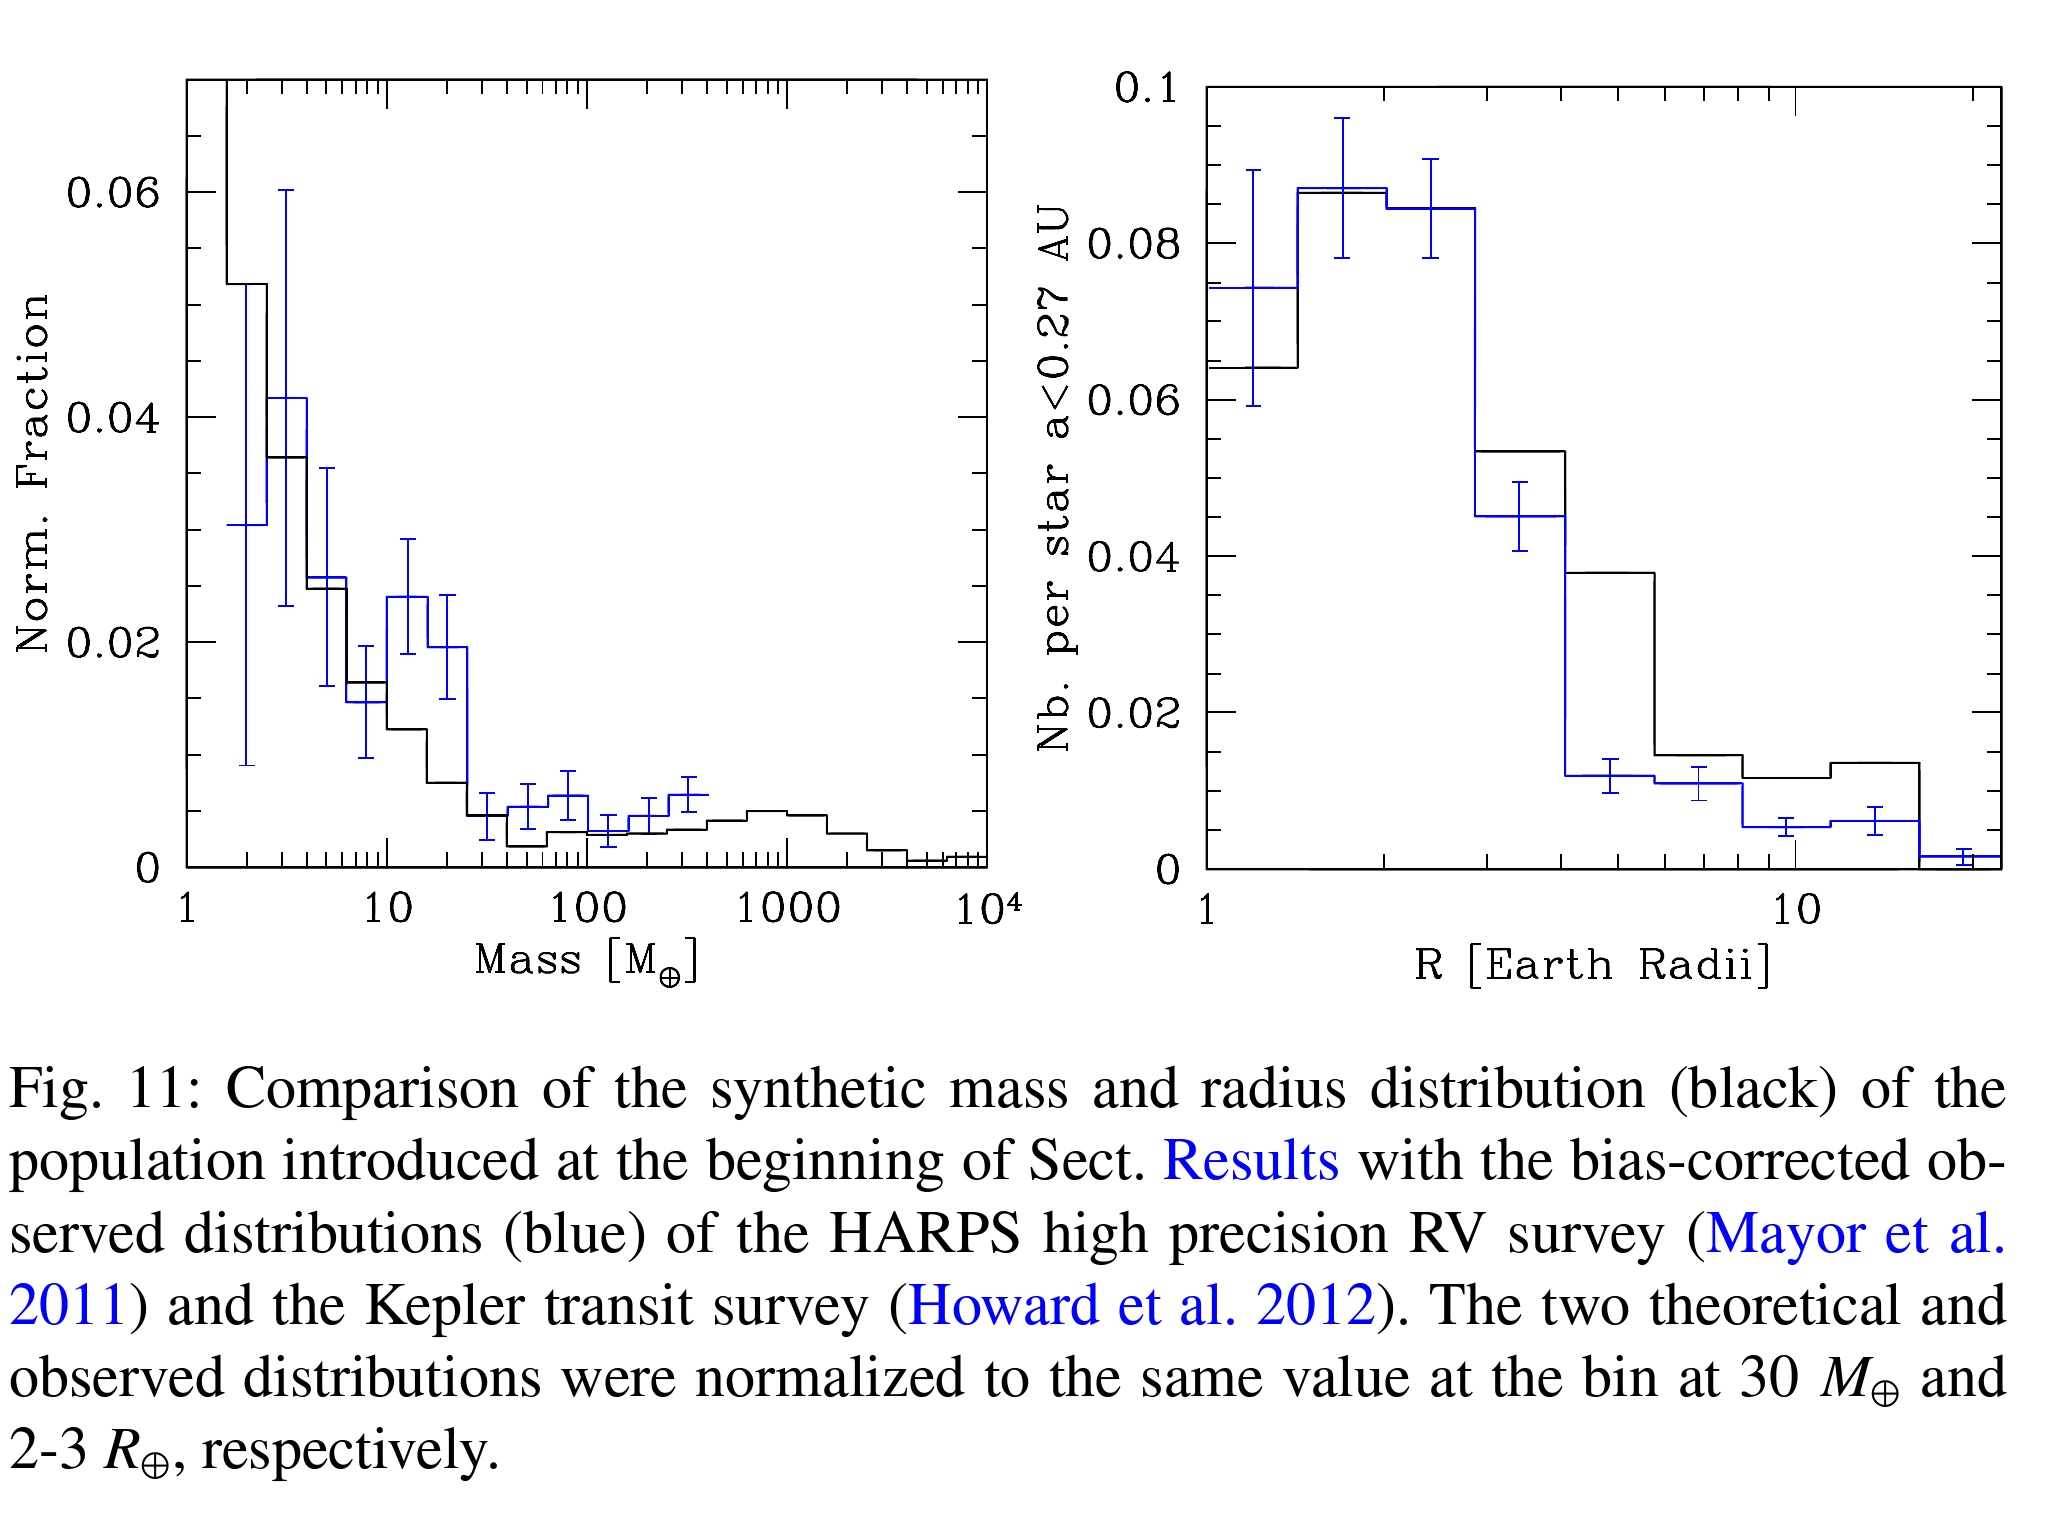
\includegraphics[trim={0cm 17cm 0 0},clip, keepaspectratio,width=0.9\textwidth]{MR-freq-obssynth}\label{}\caption{Distribuzioni di massa e raggio per popolazione planetaria sintetica (linea nera) e distribuzioni osservate tramite RV e transiti (linea blu) corrette per i bias. Da \cite{mordasini2018planetary}.}\end{figure}

\begin{figure}[!ht]
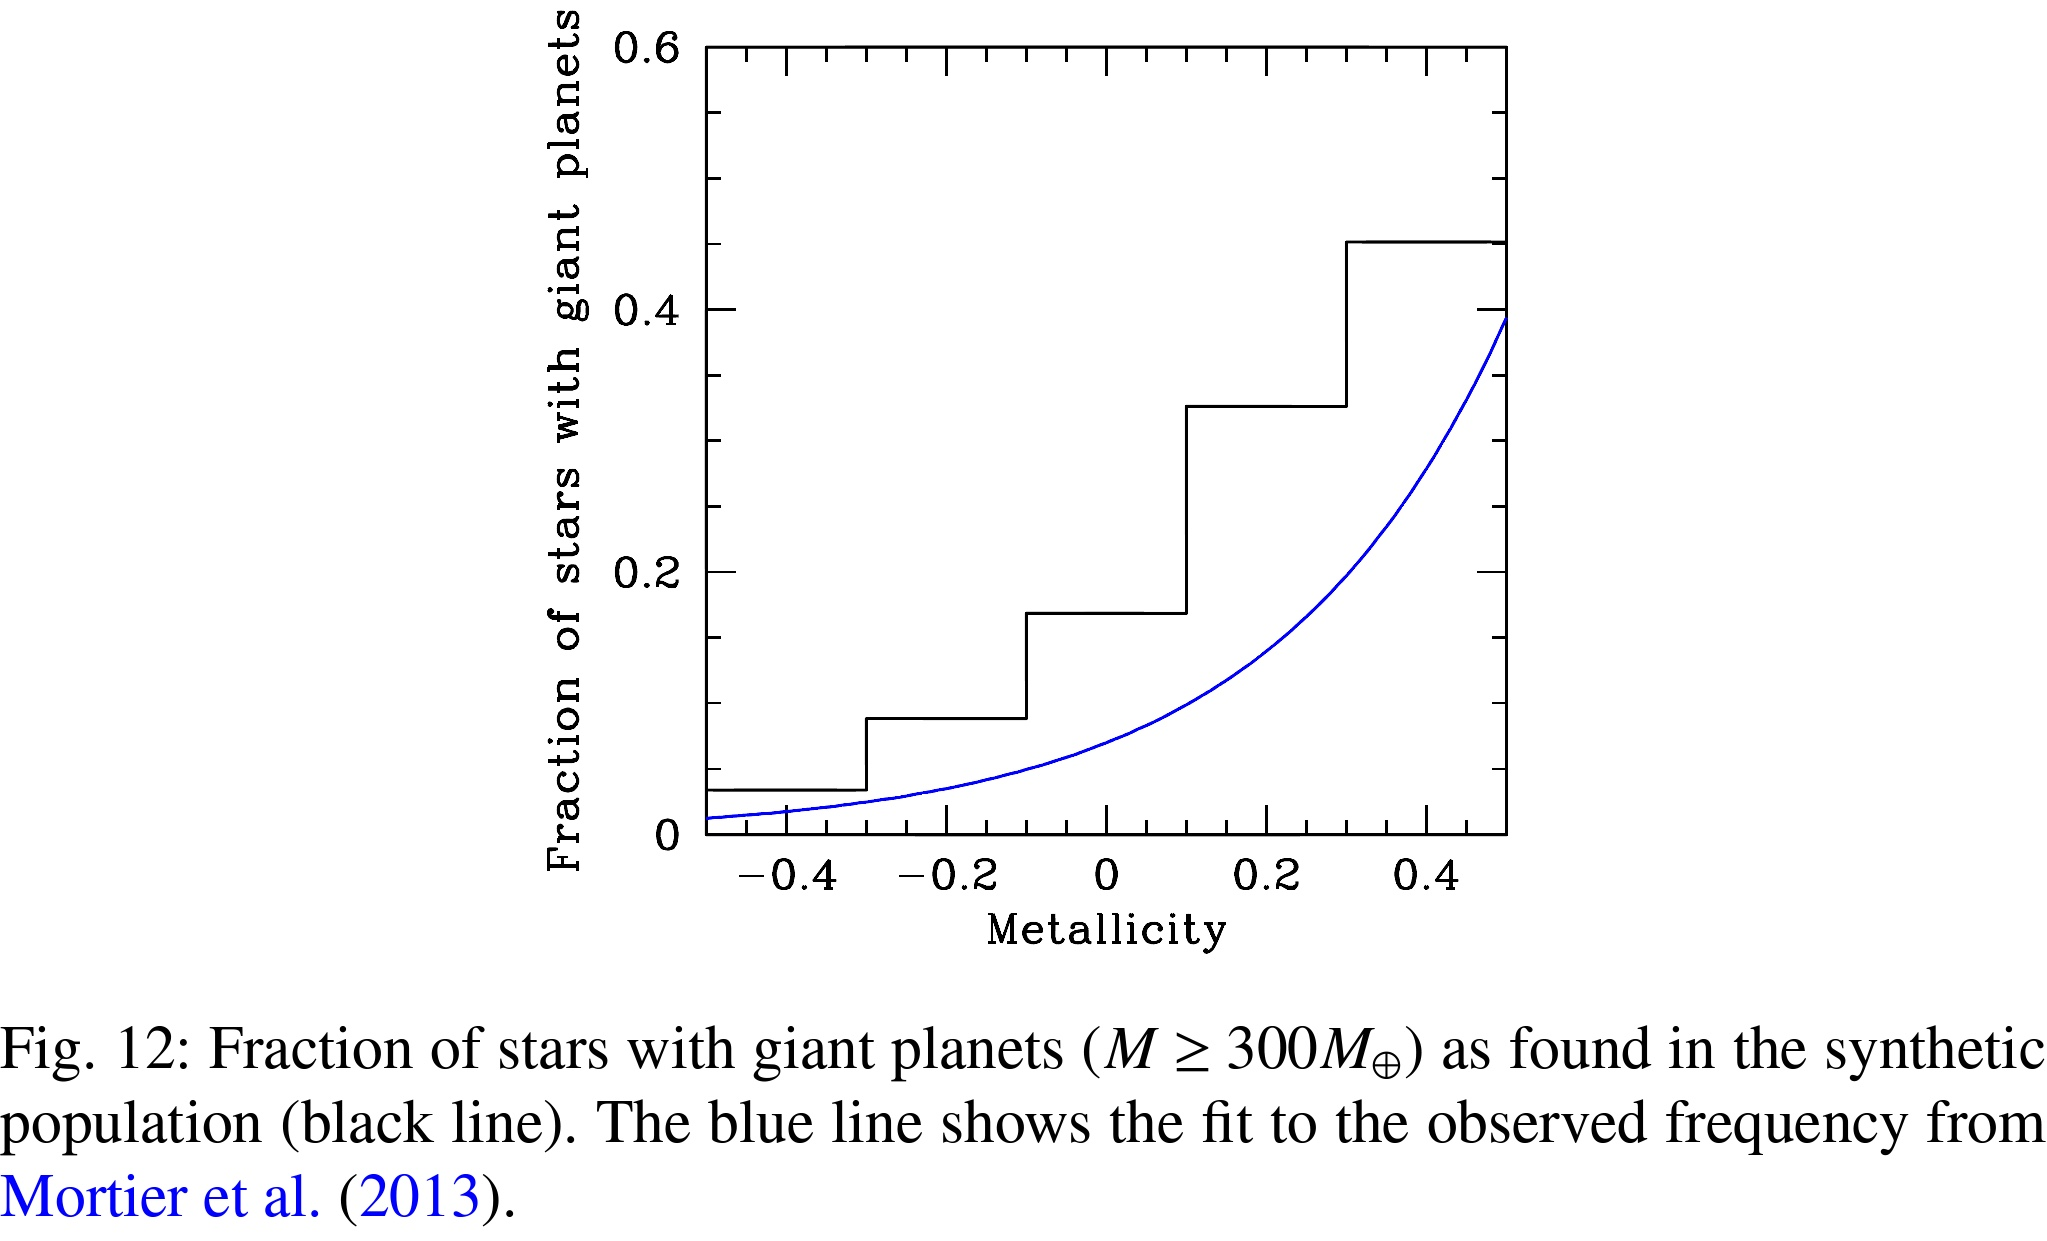
\includegraphics[trim={0cm 10cm 0 0},clip, width=0.9\textwidth,keepaspectratio]{giant-Zsynth}
\caption{Da \cite{mordasini2018planetary}. }
\end{figure}

\begin{workout}[Orbital structure and MMR: comparison simulation/observation]

\end{workout}

\begin{workout}[Comparison with stellar initial mass function]
Stelalr imf: chabrier 03, salpeter slope 1955
\end{workout}


%{\let\clearpage\relax\let\cleardoublepage\relax
%\chapter{Raffinamento dei modelli}
%}


\begin{workout}[Effects of saturation, cooling and irradiation.]
Impact of planet migration model on planetary populations: effects of saturation, cooling and stellar irradiation (??)
Outward migration helps some planets to become massive, accumulation zone at certain semiaxis, at what mass corotation saturate?
Migration of protoplanets in radiative disks
\end{workout}

\cleartorecto



{\let\clearpage\relax\let\cleardoublepage\relax
\backmatter
}
%\newgeometry{margin=60px,tmargin=20px}%%APPENDICE
%\appendix
%\part{Appendice}
%\subfile{appendix}
%\restoregeometry
\printbibliography
%\listoffigures
\ifx\versione\bozza
\woc
\erratac
\fi
\end{document}
